\documentclass[a4paper,11pt,twoside,openright,titlepage]{book}


\usepackage[perpage,bottom,ragged]{footmisc}
\usepackage[italian]{babel}
\usepackage[T1]{fontenc}
\usepackage[latin9]{inputenc}
\usepackage[Lenny]{fncychap}
\usepackage{epigraph}
\usepackage{fancyhdr}
\usepackage{graphicx}
\usepackage[twoside,bindingoffset=2.5cm]{geometry}
\usepackage{indentfirst}
\usepackage{amsmath}
\usepackage{amsfonts}
\usepackage{listings}
\usepackage{subfigure}


\hyphenation{NNSec nnsec JavaNNS}
\setlength{\headheight}{14pt}

\raggedbottom

\newcommand{\helv}{\fontfamily{phv}\fontseries{b}\fontsize{9}{11}\selectfont}
\newcommand{\figfont}{\fontfamily{phv}\fontsize{8}{10}\selectfont}

\pagestyle{fancy}
\fancyhf{}
\renewcommand{\chaptermark}[1]{\markboth{#1}{}}
\renewcommand{\sectionmark}[1]{\markright{#1}}
\renewcommand{\headrulewidth}{0.1pt}
\fancyhead[LO,RE]{\helv\leftmark}
\fancyhead[RO,LE]{\helv\rightmark}
\fancyfoot[C]{\thepage}
\fancypagestyle{plain}{\fancyhead{}\fancyfoot{}\renewcommand{\headrulewidth}{0pt}\renewcommand{\footrulewidth}{0pt}}
\clearpage{\pagestyle{empty}\cleardoublepage}
\makeatletter
\def\cleardoublepage{\clearpage
\if@twoside
	\ifodd
		\c@page
	\else
		\hbox{}
		\vspace*{\fill}
		\vspace{\fill}
		\thispagestyle{empty}
		\newpage
		\if@twocolumn
			\hbox{}
			\newpage
		\fi
	\fi
\fi}
\makeatother

\setlength{\marginparwidth}{0.75in}
\addtolength{\headwidth}{\marginparsep}
\addtolength{\headwidth}{\marginparwidth}

\bibliographystyle{alpha}


\begin{document}

\frontmatter
\thispagestyle{plain}
\begin{center}
\begin{center}

\includegraphics[scale=0.75]{img/salomone.eps}
\end{center}
Universit� degli Studi di Firenze\\
Facolt� di Ingegneria
\rule{12cm}{0.5mm}\\[0.3cm]
Corso di Laurea in\\ Ingegneria Informatica\\
\vspace{3cm}
{\begin{huge}\textbf{Protocollo sicuro per l'elaborazione di\\ dati cifrati mediante una rete neurale}\end{huge}}\\
\vspace{\stretch{1}}
\begin{large}
\textbf{Relatore:}\hspace{10pt}Piva Alessandro\hspace{\stretch{1}}\textbf{Candidato:}\hspace{10pt}Caini Michele \\
\vspace{10pt}
\textbf{Co-relatori:}\hspace{\stretch{1}}\hbox{\hspace{1pt}}\\
\hspace{50pt}Bianchi Tiziano\hspace{\stretch{1}}\hbox{\hspace{1pt}}\\
\hspace{50pt}De Rosa Alessia\hspace{\stretch{1}}\hbox{\hspace{1pt}}\\
\hspace{50pt}Orlandi Claudio\hspace{\stretch{1}}\hbox{\hspace{1pt}}\\
[3cm]
\hspace{\stretch{1}} A.A. 2006/2007
\end{large}
\end{center}

% blank-page
\thispagestyle{empty}
\hbox{\hspace{1in}}
\newpage
% / blank-page
\null\vspace{\stretch{1}}
\begin{flushright}
\setlength{\epigraphwidth}{21em}
\epigraph{
Molte volte ho osservato \\
il marmo che hanno scolpito per me - \\
un vascello con una vela ammainata \\
alla fonda in un porto. \\
In verit� ci� non rappresenta la mia destinazione \\
ma la mia vita. \\
Perch� mi fu offerto l'amore e io \\
fuggii i suoi disinganni; \\
il dolore buss� alla mia porta, ma ebbi paura; \\
mi chiam� l'ambizione, ma le opportunit� mi hanno \\
	terrorizzato. \\
Eppure continuavo a desiderare \\
di dare un significato alla mia vita. \\
E ora io so che bisogna alzare le vele \\
e prendere i venti del destino \\
dovunque conducano il vascello. \\
Dare un significato alla propria vita \\
pu� finire in follia, \\
ma la vita senza significato � la tortura \\
del senza requie e vago desiderio - \\
essa � un vascello che smania per il mare \\
e ne ha paura.\\
\flushright George Gray
}{Edgar Lee Masters, Antologia di Spoon River}
\end{flushright}
\vspace{\stretch{2}}\null
\tableofcontents
\listoffigures
% \listoftables
\chapter{Introduzione}

La necessit� crescente di sicurezza unita alla potenza classificativa delle reti neurali ha portato alla nascita di un protocollo che permettesse di sposare le due cose, in modo da ottenere reti neurali sicure grazie alla loro capacit� di operare in dominio cifrato. Lo scopo di questo protocollo � quello della classificazione remota sui dati in assenza di una terza parte fidata, che preveda un livello di interazione minimo fra le due parti coinvolte.
\paragraph{}
Da un lato, le tecniche che mirano a conseguire politiche di sicurezza si fanno di giorno in giorno pi� raffinate e permettono di esplorare terreni impensabili fino a poco tempo fa. La spinta nello studio di aspetti particolari dei cifrari, come le loro propriet� omomorfiche, permette di inquadrare questi oggetti in un'ottica del tutto nuova che prevede lo sfruttamento di tali caratteristiche per riuscire ad ottenere operazioni in chiaro senza dover passare obbligatoriamente da fasi di decifratura e conseguente cifratura. A partire da questo punto di vista nasce una \textit{nuova matematica}, che permette di operare su valori cifrati per applicare indirettamente funzioni lineari ai valori in chiaro.\\
Dall'altro lato, le reti neurali stanno prendendo sempre pi� piede in svariati ambiti e si stanno affermando come strumento potente, flessibile e preciso, utile alla classificazione dei dati e alla rappresentazione di funzioni difficilmente esprimibili o di cui, addirittura, niente ancora si conosce. Lo studio, in questo campo, sta portando alla scoperta di tecniche e algoritmi capaci di generalizzare sui dati, ottenendo cos� reti neurali in grado di dare risposte sempre pi� precise.

Il matrimonio fra queste due scienze sfocia in un protocollo che permette di mettere a disposizione degli utenti reti neurali per un utilizzo remoto, fornendo una discreta riservatezza a chi si affida al servizio e vuole proteggere i propri dati come ovviamente anche sicurezza per chi investe nella creazione e nell'addestramento delle reti neurali.\\
Un terzo elemento importante che ha permesso l'implementazione di un protocollo del genere � sicuramente l'insieme di strumenti messi a disposizione dello sviluppatore, i quali permettono di rendere realizzabili e reali un gran numero di idee: dalla teoria alla pratica, per poter toccare con mano ed esplorare una delle nuove frontiere della crittografia.

\paragraph{}
Il lavoro di tesi si propone di realizzare uno strumento che permetta di toccare con mano il protocollo in questione, indagando tanto sull'effettiva possibilit� di implementazione quanto sulle prestazioni ottenibili in ambienti reali, per dare una risposta all'ovvia domanda se questo possa o meno trasformarsi in una soluzione concreta e rappresentare un possibile futuro in questo ambito.

La discussione riguardante l'argomento si articola in tre capitoli che affrontano e descrivono rispettivamente la parte teorica, le fasi di sviluppo e i test portati avanti sul prodotto finale. Segue una breve descrizione sui contenuti di ogni singolo capitolo:
\begin{itemize}
\item \textbf{Capitolo \ref{cap:one}}: in questo capitolo � descritto il protocollo proposto e sviluppato nel lavoro di tesi; vengono discussi gli aspetti importanti di questo protocollo, gli algoritmi coinvolti e le tecniche per conseguire la sicurezza in seno tanto all'utente quanto a chi fornisce le reti neurali per l'uso remoto e sono trattati gli elementi chiave utilizzati, quali il cifrario, con le loro propriet� e caratteristiche
\item \textbf{Capitolo \ref{cap:two}}: essendo il prodotto finale un software che implementa il protocollo proposto e descritto nel capitolo \ref{cap:one} � necessario dedicarsi all'analisi della struttura del programma discutendone le fasi di progettazione, le scelte effettuate, le problematiche incontrate e le soluzioni introdotte per risolvere tali questioni, discutendo anche i mezzi utilizzati per realizzare il prodotto finale; in realt�, la trattazione non scende nei dettagli del codice spiegandone ogni singola riga o funzione, piuttosto � data una panoramica degli attori principali nel progetto e di come questi implementino soluzioni utili
\item \textbf{Capitolo \ref{cap:three}}: un software �, ovviamente, valutato in base a parametri di complessit�, al comportamento che presenta a seguito di variazioni sulle variabili d'ambiente e, perch� no, al corretto funzionamento (un programma il cui risultato non � quello atteso, anche se presenta prestazioni invidiabili � di scarso interesse): in questo capitolo � portata avanti un'analisi in base a dati sperimentali nel tentativo di estrapolare una legge che possa risultare utile a prevedere il comportamento del programma in base ad alcuni parametri predefiniti, come il fattore di quantizzazione o il numero di nodi fittizi
\end{itemize}
\paragraph{}
Sar� quindi discusso il come, a partire dal cosa, per arrivare al quanto.\\
Cosa tratta il protocollo proposto, analizzato e descritto in ogni sua sfaccettatura per capirne in linea teorica il funzionamento e poterne comprendere le problematiche, importanti anche dal punto di vista realizzativo.\\
Come questo � stato implementato, senza tralasciare le metodologie e le tecnologie utilizzate per raggiungere lo scopo, focalizzando sui modi in cui problemi affrontati in linea teorica e relative soluzioni sono stati affrontati e risolti praticamente.\\
Quanto � realmente utilizzabile il software, indici di prestazione e degenerazione dei valori in base ai parametri di ambiente, un'approssimazione del comportamento per stime a priori, cercando di estrapolare una legge che fornisca indizi sul comportamento del programma in base a variabili esterne.
\paragraph{}
La discussione si articola quindi in tre settori principali e attraverso questi guida l'analisi dalla teoria alla pratica, fornendo infine risultati concreti nella forma di un software chiamato NNSec.


\mainmatter
\chapter{Il Protocollo}\label{cap:one}
\epigraph{Qualunque cosa voi facciate sar� insignificante, ma � molto importante che voi la facciate}{Mahatma Gandhi}

Al giorno d'oggi esistono due grandi filoni dell'informatica in cui tanto si � fatto ma dove ancora tanto c'� da fare, in particolare il ramo della crittografia e quello dell'apprendimento automatico. Il primo rappresenta una corsa contro il tempo in cui, giorno dopo giorno, nuove tecniche vengono scoperte o raffinate e altre ancora violate, rese praticamente inutilizzabili. Nell'ambito dell'apprendimento, invece, sono stati fatti passi da gigante proprio negli ultimi decenni e le potenzialit� di strumenti come le reti neurali sono ormai evidenti. L'articolo descritto in \cite{proto} rappresenta un tentativo di sposare le due cose ed � il punto di partenza del lavoro di tesi. In questo articolo � introdotto un protocollo per l'uso remoto di reti neurali che fornisca sicurezza (sar� spiegato in seguito cosa ci� significhi realmente e cosa comporti) tanto a chi mette a disposizione la rete neurale quanto a chi la sfrutta.

Lo sviluppo del software, rappresentazione concreta e finale del lavoro di tesi, si � concentrato sul protocollo proposto, cercando di sviscerarne ogni aspetto e tramutandolo in classi e relazioni fra queste. Ma lo sforzo non � stato a senso unico. Infatti, come sar� illustrato in una sezione dedicata, dalla fase di codifica ha potuto beneficiare il protocollo stesso in merito ad alcune sue sfaccettature, a seguito di alcune osservazioni sugli algoritmi coinvolti e loro conseguenti generalizzazioni.

Ovviamente, per quanto il lavoro di tesi non sia sfociato nel protocollo di seguito descritto ma sia partito da esso, � necessario dare una descrizione di quest'ultimo che permetta di capirne i retroscena, le motivazioni e i possibili utilizzi. In questo capitolo, quindi, sar� discusso il protocollo sopra citato, cercando di darne una breve ma esaustiva descrizione.

\newpage

\section{Scopo}\label{sec:aim}
Volendo dare una descrizione un po' semplicistica, le reti neurali sono un potente strumento, relativamente moderno, utile per la classificazione dei dati. Questi oggetti sono in grado di racchiudere dentro la loro struttura interna fatta di livelli intermedi nascosti un'informazione espressa in termini di pesi sui collegamenti fra i nodi componenti, cos� da riuscire a discriminare su un insieme di dati in ingresso assegnando loro una determinata classe. Le reti neurali vanno ovviamente create e addestrate, per poter insegnare loro come classificare i dati in ingresso ed essere quindi utilizzate allo scopo.

Il protocollo proposto su cui si � sviluppato il lavoro di tesi, discusso in \cite{proto}, propone un modello in cui due entit� indipendenti desiderano l'una di mettere a disposizione una rete neurale (quindi, prendendosi anche il compito di crearla e allenarla) e l'altra di sfruttare il servizio offerto. La necessit�, per�, � che ci� avvenga in sicurezza. Cosa realmente significhi questa parola, poi, sar� ampiamente discusso.\\
L'idea alla base di questo nuovo protocollo � quella di non affidarsi alle soluzioni generiche per SMC (Secure Multi-Party Computation) per la computazione, come discusse in \cite{yao1982psc} e \cite{goldreich1987pam}, ovvero cercare di evitare di ricorrere a tecniche che introducessero nel protocollo stesso un alto grado di interazione fra le parti. Infatti, SMC mira a risolvere problematiche che coinvolgono pi� attori, senza ricorrere ad una terza parte ma piuttosto utilizzando protocolli che prevedono un alto grado di collaborazione fra i diversi soggetti. Queste tecniche si sono rivelate piuttosto inefficienti quando applicate a specifiche situazioni come quella in esame. Infatti, per loro stessa natura, impongono una decisa collaborazione fra client e server per la computazione delle funzioni di attivazione o uscita di un nodo e, di conseguenza, un alto carico in termini di tempo, memoria e banda spese per ottenere il risultato. Piuttosto, questo protocollo cerca di introdurre un modello che limiti le interazioni fra client e server, basandosi su tecniche di cifratura che presentano propriet� omomorfiche cos� da permettere di ottenere direttamente tramite operazioni nel dominio cifrato tutte le computazioni lineari. Per le funzioni non lineari, invece, come gi� accennato, bisogna ricorrere obbligatoriamente ad una interazione fra le parti.\\
Tutto ci� � ottenuto in modo da assicurare due cose:
\begin{itemize}
\item chi mette a disposizione la rete neurale potr� contare sul fatto che la sua conoscenza rimarr� privata e non sar� diffusa permettendone duplicati; in altri termini, l'attenzione � focalizzata nel tentativo di evitare che un ipotetico attaccante possa ricostruire la rete neurale messa a disposizione per l'uso remoto semplicemente sottoponendo ad essa determinati input e risalendo dai risultati ottenuti alla struttura interna della rete stessa
\item chi sfrutta la rete neurale messa a disposizione avr� la certezza che i suoi dati non siano diffusi o scoperti, dove per dati si intendono i valori di ingresso e di uscita della rete neurale e non altri dati potenzialmente sensibili come i dati anagrafici; si possono immaginare i dati sottoposti alla rete neurale come descrizione di sintomi e il risultato ottenuto come una conferma o meno sul fatto che l'utente abbia una malattia grave: esistono allora molti casi gi� in questo semplice esempio in cui occultare tali dati pu� risultare molto importante dal punto di vista dell'utente
\end{itemize}
Nel primo caso, quindi, � protetto l'investimento fatto da chi crea e addestra la rete neurale e non vuole che terzi possano ottenerne una copia identica a partire da quella proposta e da un'analisi del suo comportamento. Nel secondo caso, invece, sono protette le informazioni relative all'utente remoto di tali reti neurali, ovvero sono occultati i valori sottoposti in ingresso ad esse e i risultati ottenuti.

\section{Mattone su mattone}
Prima di descrivere nei particolari il protocollo proposto, � necessario parlare di alcuni aspetti di contorno utili per poter capire al meglio quanto sar� detto. Questa sezione, quindi, presenta tutto ci� che pu� essere pensato come le fondamenta, o meglio l'insieme di mattoni con cui il protocollo stesso sar� costruito, mattone dopo mattone.

\subsection{Reti neurali}\label{subsec:nn}
Esistono svariati tipi di rete neurale, ognuna adatta a scopi pi� o meno specifici e modellabile secondo necessit�. Per approfondimenti su tale argomento e sull'apprendimento automatico in generale, si consiglia la lettura di \cite{RussellNorvig} e \cite{Mitchell}. Di seguito saranno illustrate le diverse tipologie di reti neurali interessate dal protocollo proposto e che con quest'ultimo possono essere utilizzate realmente e praticamente.\\
Prima di tutto, si osservi che le reti neurali sono potenti strumenti per la classificazione dei dati e permettono di modellare un gran numero di funzioni conosciute o meno. Al giorno d'oggi � noto che, dal punto di vista teorico, una rete neurale pu� approssimare con precisione arbitraria un insieme molto ampio di funzioni, a seconda della struttura interna della rete neurale utilizzata, del numero di livelli intermedi e del numero di nodi in essi presenti. Queste reti sono spesso fornite con buoni algoritmi di apprendimento, hanno un'alta resistenza al rumore e generalizzano in modo corretto su un gran numero di esempi non visti, risultando ottimi strumenti per riuscire a descrivere anche funzioni sconosciute. Si pu� infatti pensare ad una rete neurale come ad una scatola nera che in base ai processi di apprendimento modella al suo interno una serie di relazioni fra i nodi, cos� da essere in grado di riprodurre le funzioni che hanno generato i dati proposti in queste fasi. Potenzialmente, quindi, questi oggetti possono anche arrivare ad approssimare con una certa precisione fenomeni descritti da funzioni al momento sconosciute all'uomo, ma di cui quest'ultimo conosce gli ingressi e le uscite senza essere ancora riuscito a ricavare o dimostrare una relazione valida fra di essi.

Esistono comunque vari tipi di reti neurali e non tutte sono utilizzabili con il protocollo sviluppato in NNSec. In particolare, possono essere utilizzati solo percettroni e reti neurali di tipo feed-forward, descritte di seguito. Nella pratica possono essere descritte un numero molto maggiore di reti neurali rispetto a quelle che NNSec � realmente in grado di trattare, grazie alla grammatica sviluppata per descrivere tali oggetti, ma il fatto che una rete neurale si possa sottoporre in ingresso al software non implica necessariamente che questa si comporti come atteso una volta utilizzata.

\paragraph{Percettrone.}
Il percettrone, riportato in figura \ref{fig:perc} � una delle reti neurali pi� elementari. Non presenta livelli intermedi, ma solamente un insieme di nodi di ingresso collegati a loro volta ad un nodo di uscita, direttamente. Questo modello pu� in realt� anche essere generalizzato aggiungendo pi� nodi di uscita, ma la trattazione sar� fatta sul modello con singolo nodo di uscita senza perdere di generalit�.\\
\begin{figure}
\centering
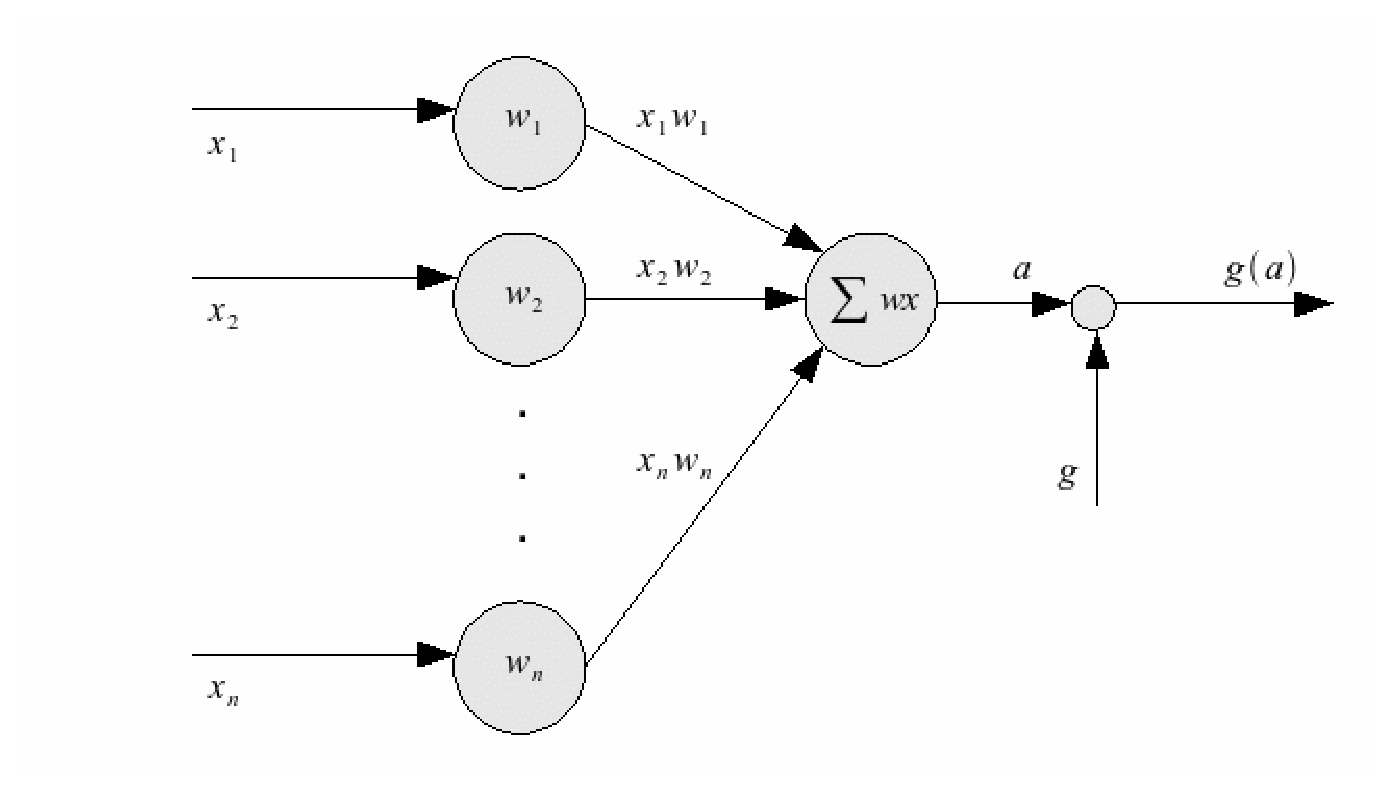
\includegraphics[scale=0.55]{img/perceptron.eps}
\caption{\figfont il percettrone}\label{fig:perc}
\end{figure}
Il percettrone pu� discriminare fra due classi di appartenenza, approssimando funzioni che di fatto classificano gli ingressi associandoli ad una classe piuttosto che ad un'altra. Il valore di uscita � calcolato come combinazione lineare dei valori in ingresso pesati in base ai valori presenti sui collegamenti fra nodi. Il valore cos� ottenuto pu� essere ulteriormente elaborato tramite l'uso di una funzione di attivazione detta $ g $, come ad esempio la funzione sigmoide o la funzione segno. Quindi, il valore sul nodo terminale non sar� necessariamente la combinazione lineare dei valori pesati in ingresso, a meno che la funzione di attivazione non sia rappresentata dall'identit�.\\
La forma matematica per il discriminante (ovvero il valore associato al nodo di uscita prima dell'elaborazione) � data dalla seguente espressione: $ a(x) = \bar{w}^T\bar{x} + w_0 $ , dove $ \bar{x} $ rappresenta il vettore di ingresso e $ \bar{w} $ il vettore dei pesi sui collegamenti, mentre $ w_0 $ � la soglia associata al nodo. Per ottenere il valore realmente associato al nodo di uscita, basta applicare al discriminante la funzione di attivazione $ g $, ovvero ricavare: $ g(a) $. L'uscita � associata alla classe $ c_1 $ se $ g(a) \geq w_0 $, oppure alla classe $ c_2 $ se $ g(a) < w_0 $. In realt�, il valore $ w_0 $ pu� essere inglobato nei vettori $ \bar{x} $ e $ \bar{w} $, ottenendo due vettori alternativi $ \bar{x}' = [\bar{x}\mid 1]^T $ e $ \bar{w}' = [\bar{w}\mid w_0]^T $, da cui si ottiene $ a(x) = \bar{w}'^T\bar{x}' $; in questo caso, la soglia che discrimina nell'associazione dei valori in ingresso ad una classe piuttosto che ad un'altra � data dal valore $ 0 $. In caso esista la necessit� di trattare con pi� classi di appartenenza, ovvero nei casi in cui siano presenti pi� nodi di uscita, il metodo pu� essere facilmente generalizzato ripetendo quanto illustrato sopra per ogni nodo di uscita del percettrone.

\paragraph{Reti Feed-Forward}
Il percettrone ha molte limitazioni, la pi� importante delle quali � che esso non riesce ad operare correttamente su insiemi di dati che non siano linearmente separabili in due classi di appartenenza, come ad esempio la funzione \textit{xor}. Da queste limitazioni nascono le reti feed-forward con un numero arbitrario di livelli intermedi nascosti, riportate in figura \ref{fig:nn}.\\
\begin{figure}
\centering
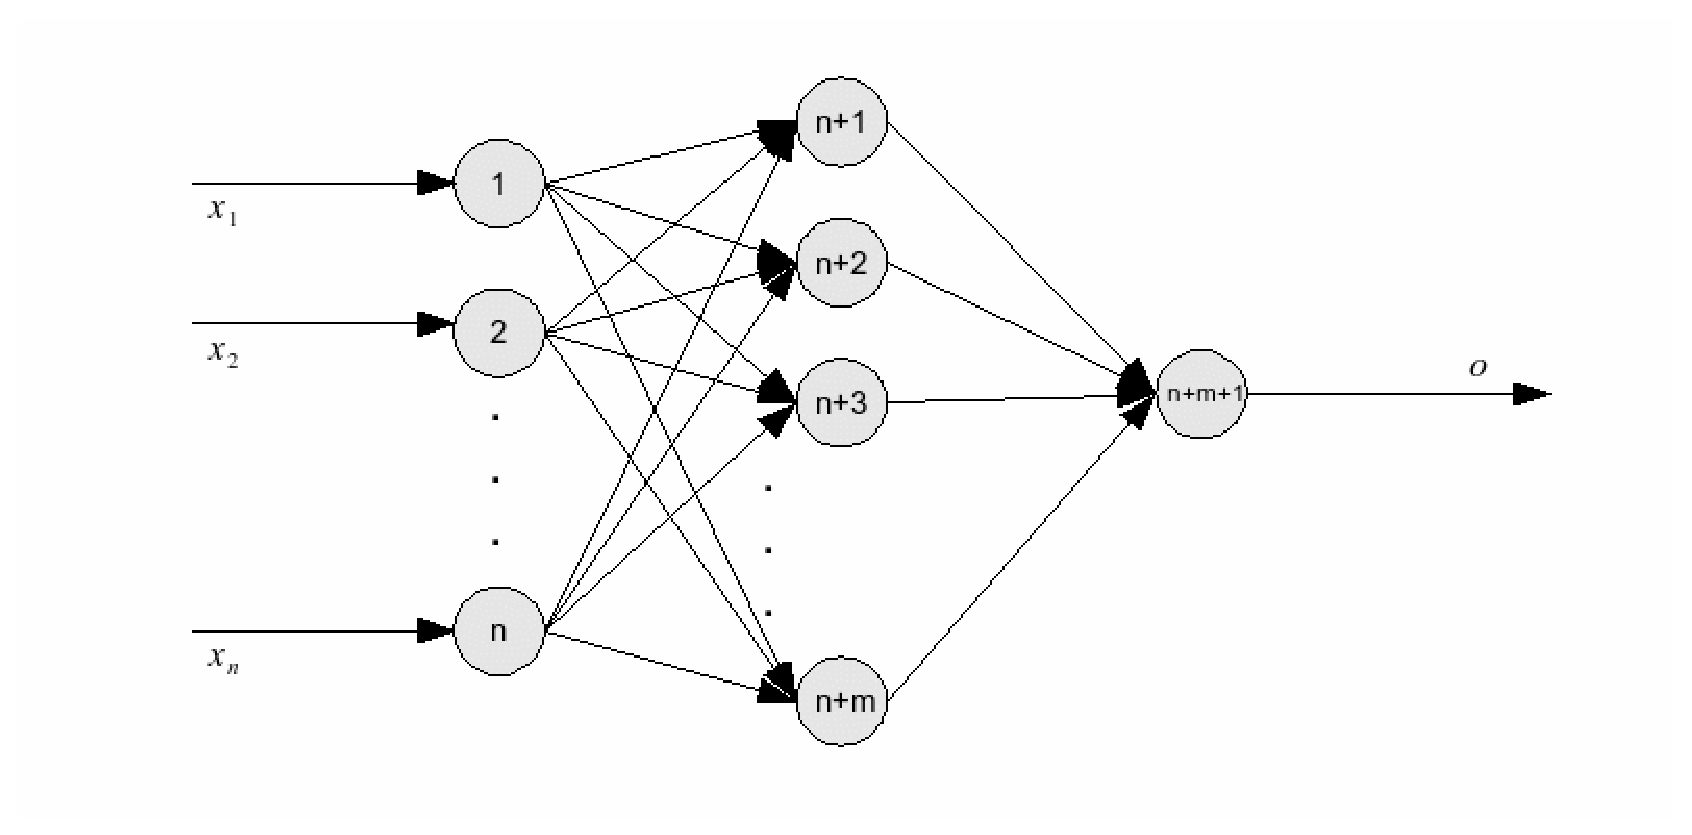
\includegraphics[scale=0.45]{img/nn.eps}
\caption{\figfont rete neurale feed-forward}\label{fig:nn}
\end{figure}
Nelle reti di tipo feed-forward la propagazione dei segnali avviene unicamente, in maniera continua, nella direzione che conduce dagli ingressi alle uscite, mentre nelle reti ricorrenti (non feed-forward) tale propagazione pu� anche manifestarsi da uno strato neurale successivo ad uno precedente, oppure tra neuroni appartenenti ad uno stesso strato, e persino tra un neurone e s� stesso, generando quindi cicli. Le reti feed-forward, invece, si caratterizzano proprio per l'assenza di cicli. In questi tipi di rete, i nodi si dividono in tre categorie: nodi di ingresso, ovvero i nodi che ricevono i valori di ingresso dall'esterno; nodi di uscita, ovvero i nodi che presentano il risultato dell'elaborazione; nodi nascosti, tutti i nodi che non sono n� di ingresso n� di uscita. Ogni nodo poi riceve collegamenti da nodi appartenenti a livelli precedenti, ad eccezione ovviamente dei nodi di ingresso, e propone collegamenti diretti verso nodi che risiedono in livelli successivi, ad eccezione dei nodi di uscita; nessun altro tipo di collegamento � permesso. Immaginando di numerare in ordine crescente i nodi (come evidenziato in figura \ref{fig:nn}), si possono descrivere le reti feed-forward come quelle reti in cui ogni nodo $ n $ riceve collegamenti provenienti solo da nodi con indice $ m $ tale che $ m < n $ e propone collegamenti esclusivamente verso nodi con indice $ h $ tale che $ h > n $. Queste direttive, seppure pongano limiti sulla libert� di strutturare una rete a piacimento, permettono di avere modelli pi� facilmente analizzabili tanto in linea teorica che all'interno di un software.\\
Il valore associato al $ j $-esimo nodo nascosto appartenente all'$ i $-esimo livello intermedio � ottenuto ricavando prima di tutto la combinazione lineare degli $ l $ valori in ingresso pesati a seconda dei valori di collegamento, ovvero:
$$ a_j^{(i)} = \sum^l_{k = 1}w_{jk}^{(i)}x_k $$
In questo caso, $ w_{jk}^{(i)} $ indica il peso associato all'arco proveniente dal $ k $-esimo nodo appartenente al livello precedente a $ i $ e diretto al $ j $-esimo nodo del livello $ i $. Come per il percettrone, i singoli nodi possono avere una funzione di attivazione e/o di uscita, anche immaginabile come funzione unica associata al singolo nodo e detta $ g $. Il valore risultante per il nodo in questione, ottenuto dalla computazione del valore associato a tale nodo, � ricavato come segue:
$$ z_j^{(i)} = g\left( a_j^{(i)}\right) $$
Ovviamente, iterando su tutti i nodi nascosti fino a raggiungere i nodi di uscita e applicando lo stesso procedimento anche a quest'ultimi, si ottiene il risultato finale della computazione all'interno della rete neurale.

\paragraph{Funzioni.}
Per quanto riguarda le funzioni di attivazione dei singoli nodi, queste sono solitamente un insieme limitato e ben definito comprendente quelle che meglio si adattano allo scopo.
\paragraph{}
Fra le pi� usate, la funzione sigmoide, ovvero:
$$ f(a) = \frac{1}{1 + e^{-a}} $$
Il termine sigmoide significa ``a forma di S''. Questa funzione conduce  dall'intervallo $ (-\infty, \infty) $ in $ (0, 1) $, come riportato in figura \ref{fig:sigmoid}, la quale mette meglio in evidenza anche la natura stessa del suo nome.
\begin{figure}
\centering
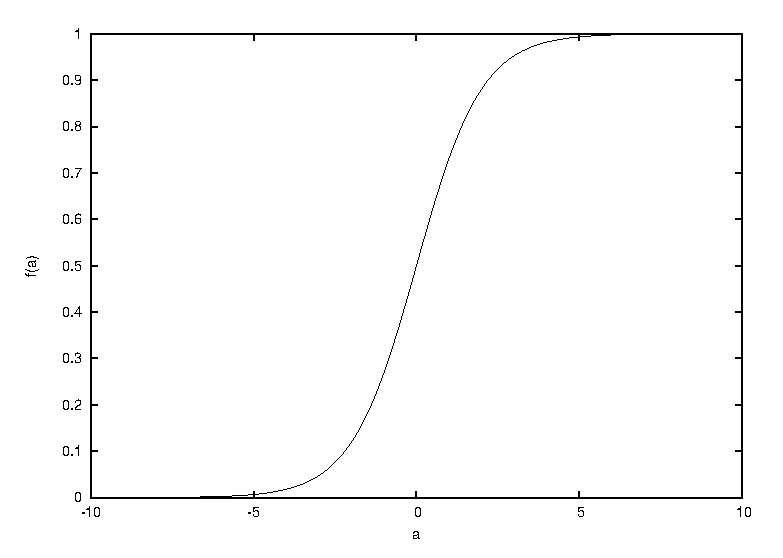
\includegraphics[scale=0.65]{img/sigmoid.eps}
\caption{\figfont funzione sigmoide}\label{fig:sigmoid}
\end{figure}
Si osservi che nei casi in cui il parametro $ a $, ovvero la somma lineare dei valori pesati in ingresso al nodo, si mantiene all'interno di un intervallo limitato intorno allo zero, questa funzione approssima una funzione lineare e rende i singoli nodi molto sensibili alle piccole variazioni. Invece, per valori di $ \vert a \vert $ superiori ad una certa soglia, la funzione sigmoide risulta quasi completamente insensibile alle variazioni, dato che essa presenta due asintoti orizzontali per $ a\rightarrow\pm\infty $
\paragraph{}
Un'altra funzione spesso usata � la funzione segno, o funzione di Heaviside, anche definita come segue:
$$ sign (x) = \left\{
\begin{matrix}
-1, & x < 0 \\
0, & x = 0 \\
+1, & x > 0
\end{matrix}
\right. $$
Questa funzione non � particolarmente complessa e si limita ad estrapolare il segno del suo valore in ingresso, permettendo di rappresentare l'intervallo $ (-\infty, \infty) $ attraverso i soli valori appartenenti all'insieme $ \left\{-1, 0, 1\right\} $.\\
La funzione segno viene spesso usata come funzione di attivazione per il percettrone, dove si discrimina fra classi di appartenenza a seconda che il valore associato al nodo di uscita sia maggiore o minore di zero come spiegato in questa stessa sezione.
\paragraph{}
Ci sono decine di funzioni utilizzate durante l'allenamento e l'uso di reti neurali e le due descritte sopra sono solo alcuni esempi delle pi� diffuse. Inoltre, la funzione segno e la funzione sigmoide sono anche le uniche due funzioni supportate in NNSec per il calcolo dei valori di attivazione dei nodi, grazie alle loro caratteristiche di anti-simmetria che le rendono particolarmente interessanti come illustrato in sezione \ref{subsec:req}.

\subsection{Requisiti dell'applicazione}\label{subsec:req}
Lo scenario considerato nel protocollo � quello in cui due utenti, Alice e Bob, dispongono rispettivamente di un insieme di dati e di un classificatore (ovvero, una rete neurale adeguatamente creata e addestrata). Alice � interessata alla classificazione dei propri dati sulla base delle conoscenze acquisite da Bob.

Sono da tralasciare, in quest'ottica, le soluzioni che prevedono l'invio da parte di Alice dei suoi dati a Bob per la classificazione e, viceversa, l'invio da parte di Bob della rete neurale ad Alice. Infatti, se da un lato Alice non gradirebbe rivelare i dati coinvolti (intesi come valori di ingresso e di uscita della rete neurale) a Bob, cos� quest'ultimo non gradirebbe uno sforzo da parte di Alice mirato a rivelare la struttura della rete neurale in modo da duplicarla (si suppone infatti che Bob abbia speso tempo e denaro per preparare la sua rete), come spiegato in sezione \ref{sec:aim}. Allo stesso modo, � da escludere il caso in cui si preveda l'utilizzo di una terza parte fidata (anche detta TTP, Trusted Third Party) che prelevi la rete neurale da Bob e i dati di ingresso da Alice per restituire infine il risultato ottenuto a quest'ultima: sar� difficile trovare un terzo elemento fidato per entrambi laddove Alice e Bob non si fidano l'un l'altro.\\
Lo scopo del protocollo � la classificazione remota dei dati che rispetti i vincoli sopra descritti ricorrendo a tecniche di crittografia che sopperiscano alla mancanza di una terza parte fidata. Come altri protocolli presenti in letteratura, anche questo si basa sul fatto che tanto Bob quanto Alice siano semi-onesti, ovvero seguano correttamente il protocollo ma possano allo stesso tempo analizzarlo in corso d'opera cercando di recuperare informazioni riguardanti l'altra parte coinvolta. Si suppone anche che Alice e Bob stiano comunicando attraverso un canale sicuro (privato e autenticato).

Di seguito � riportata una lista dei requisiti richiesti da un protocollo del genere, dove viene anche indicato se quello proposto come base del lavoro di tesi soddisfa il punto in questione o meno.

\paragraph{Correttezza.}
Ci� significa che Alice desidera avere una corretta classificazione in merito ai propri dati. Questo, nel protocollo proposto, non � possibile assicurarlo in alcun caso. Infatti, se Bob prevede di classificare i dati non solo in base alle informazioni in essi contenute ma anche in base ad altri fattori esterni, niente pu� fare il protocollo per correggere il risultato o rivelare il tentativo di falsificazione. In altri termini, se la rete neurale messa a disposizione da Bob non si comporta come dovrebbe perch� manomessa, il protocollo non potr� fare fronte a questa tipologia di situazioni. A seguito di questa eventualit� altre tecniche dovrebbero essere introdotte per porre rimedio, come ad esempio la possibilit� di ricorrere a prove di Zero-Knowledge (descritte in \cite{goldreich2001fcb}) per assicurare che ogni passaggio sia svolto correttamente.
\begin{itemize}
\item \textit{Sicurezza per Alice.} I dati di Alice sono completamente al sicuro. In realt�, i valori forniti da Alice sono in forma cifrata ed essa riceve a sua volta un risultato ancora in forma cifrata. Inoltre, in nessun momento durante l'interazione fra Bob e Alice, il primo ha modo di accedere ad una forma originale o composita dei dati che non sia cifrata e tutti i punti del protocollo che prevedono una decifratura dei dati impongono anche che questa sia messa in pratica da Alice che, a sua volta, cifrer� nuovamente tali dati prima di restituirli a Bob. Quindi, la sicurezza di Alice risiede in quella del cifrario sottostante.
\item \textit{Sicurezza per Bob.} Per quanto riguarda Bob, la sicurezza dal suo punto di vista consiste nel proteggere la propria esperienza racchiusa nella rete neurale offerta. Di conseguenza, ci� che sta a cuore a Bob � il non rivelare la struttura della rete neurale, riuscendo cos� ad impedirne la riproduzione da parte di terzi. Infatti, supponendo che Alice possa eseguire un numero arbitrario di volte il protocollo, essa pu� scoprire informazioni importanti sulla conformazione della rete neurale sottoponendo alla rete degli ingressi specifici e, quindi, pu� potenzialmente riprodurre la rete neurale di Bob. Questo discende dal fatto che a partire dagli ingressi e dal risultato di una determinata computazione si pu� sempre scoprire qualcosa in merito alla funzione coinvolta (questo � ci� su cui si basa la teoria delle reti neurali, del resto). Una buona domanda, in ogni caso, � quante interazioni siano necessarie per poter risalire alla struttura interna della rete.\\
A questo proposito � interessante focalizzarsi su cosa pu� essere importante proteggere dal punto di vista di Bob, per rendere difficile se non impossibile la violazione della sua conoscenza.
\item \textit{Struttura.} Una rete neurale feed-forward � composta da un certo numero di nodi connessi fra loro, come descritto in sezione \ref{subsec:nn}. Il protocollo � pensato per proteggere completamente il modo in cui i neuroni sono connessi e parzialmente anche il loro numero, cos� che Alice possa solo venire a conoscenza di un limite superiore $ B $ di questo numero. Il valore di $ B $ pu� essere impostato da Bob per rendere allo stesso tempo efficiente e sicuro dal suo punto di vista il protocollo stesso. In ogni caso, la necessit� di sicurezza da parte di Bob incide inevitabilmente sulle prestazioni del protocollo.
\item \textit{Risultato dei nodi nascosti.}
Potrebbe essere utile nascondere il risultato delle computazioni intermedie sui nodi nascosti, utili a raggiungere il risultato finale. Dato un nodo con una funzione di attivazione sigmoidale, � possibile quindi dividere il risultato in due parti, una che pu� essere completamente protetta, mentre l'altra sar� parzialmente rivelata. Le due parti sono:
\begin{itemize}
\item \textit{Stato del neurone.} In relazione al segno della somma pesata degli ingressi, ogni neurone pu� essere attivo o meno. questa informazione pu� essere completamente nascosta, variandola con probabilit� al cinquanta per cento. In altri termini, � possibile cambiare con cadenza non definita a priori il segno di tale valore cos� da farlo apparire completamente casuale ad Alice.
\item \textit{Valore associato.} Il parametro di attivazione relativo ad ogni neurone ha anche un valore oltre che un segno, il quale d� informazione su quanto un determinato nodo sia realmente attivo o meno. Questo valore non sar� protetto, ma Alice non avr� modo di capire quale neurone sia legato ad uno specifico parametro. Infatti, questa informazione sar� occultata attraverso tecniche di permutazione dei nodi intermedi, come illustrato in seguito.
\end{itemize}
\end{itemize}

\paragraph{Complessit� di interazione.}
Ogni scenario ideale per situazioni del genere non prevede alcuna interazione fra le parti. Questo non � il caso del protocollo proposto, che invece presenta una complessit� costante dovuta alle interazioni necessarie. In particolare, sono presenti interazioni fra Alice e Bob in quantit� strettamente proporzionale al numero dei livelli intermedi, alla luce del fatto che per ogni singolo nodo potrebbe esserci la necessit� di computare un valore di attivazione e/o di uscita (operazione che necessariamente deve essere portata a termine da Alice). Sotto quest'ottica, � possibile dire che il numero di interazioni � lineare rispetto al numero di livelli intermedi e cresce in modo proporzionale a quest'ultimo.

\subsection{Il cifrario}\label{subsec:cip}
Dietro a un grande protocollo che mira a conseguire la sicurezza, risiede un grande cifrario. In questo caso, un cifrario risultato dallo sforzo congiunto di pi� persone quali Paillier, Damg\aa rd e Jurik. Per approfondimenti sull'argomento, sono consigliate le letture di \cite{paillier} e \cite{brics}, dove viene analizzato dal punto di vista matematico il cifrario e alcune modifiche ad esso applicabili, insieme ad un'ampia discussione che analizza e approfondisce lo studio della complessit�.\\
Di seguito, saranno discussi gli aspetti pi� interessanti relativi al cifrario utilizzato.
\paragraph{Setup.}
Per l'implementazione del protocollo proposto � necessario uno schema di cifratura a chiave pubblica/privata con propriet� omomorfiche e probabilistiche. La scelt� � ricaduta sulla versione modificata da Damg\aa rd-Jurik (proposta in \cite{brics}) dello schema di cifratura di Paillier (discusso in \cite{paillier}. Questo cifrario � basato sulla difficolt� nello scoprire il residuo $ n $-esimo di un elemento in modulo $ n^{s + 1} $, dove $ n $ � un modulo RSA. Di fatto, la difficolt� nel rompere una determinata chiave � legata alla difficolt� nella fattorizzazione di numeri molto grandi. Per approfondimenti sugli argomenti legati alla crittografia, fare riferimento a \cite{goldreich2001fcb} e \cite{goldreich2004fci}.\\
Per ottenere ci�, � richiesta una fase di pre-elaborazione in cui vengono stabiliti alcuni parametri fondamentali. In particolare, sono selezionati due numeri primi $ p $ e $ q $ sufficientemente grandi da cui � calcolato il prodotto $ n = pq $ che rappresenta la chiave pubblica; la chiave privata, invece, detta $ \lambda $, � data dal minimo comune divisore tra $ (p - 1) $ e $ (q - 1) $.
\paragraph{Cifratura.}
Sia $ m \in \mathbb{Z} $ il testo in chiaro e $ s $ tale che $ n^s > m $, sia $ r $ un valore casuale tale per cui $ r \in \mathbb{Z}^*_{n^s} $ (ovvero $ r $ � compreso nell'insieme dei valori appartenenti a $ \mathbb{Z} $ e relativamente primi con $ n^s $), la versione cifrata $ c $ di $ m $ � data dalla formula:
$$ c = E_{pk} (m, r) = (1 + n)^mr^{n^s}\;mod\;n^{s + 1} $$
\paragraph{Decifratura.}
La funzione di decifratura $ D_{sk} $, invece, dipende solamente dal testo cifrato e non c'� bisogno di conoscere il valore casuale $ r $ in questa fase. Ovviamente, solo il possessore della chiave privata potr� risalire al testo in originale. Per chiarimenti sulla fase di decifratura, si faccia riferimento a \cite{paillier} e \cite{brics}.
\paragraph{}
Uno dei grossi vantaggi del cifrario utilizzato � dato dal fatto che solamente il parametro $ n $ deve essere fissato, mentre $ s $ pu� essere aggiustato in base al testo in chiaro. In altre parole, diversamente da molti cifrari dove bisogna scegliere la dimensione del testo in chiaro imponendola minore di $ n $, in questo caso si pu� scegliere $ m $ arbitrariamente grande e quindi operare su $ s $ per fare in modo che sia $ n^s > m $. Questo ovviamente si ripercuote sul protocollo traducendosi in una maggiore libert� sulla scelta della dimensione dei valori $ m $.
\paragraph{Propriet� omomorfiche.} 
Come detto, il cifrario proposto soddisfa alcune propriet� omomorfiche che possono rappresentare, a seconda dei punti di vista, un aspetto problematico o interessante di un sistema crittografico. In questo caso, come si pu� capire, la cosa � ben voluta.\\
Supponendo di avere due elementi in chiaro detti $ m_1 $ e $ m_2 $, indicando con $ E(m) $ la cifratura del messaggio in chiaro $ m $ e con $ D(c) $ la sua decifratura, sono soddisfatte le seguenti uguaglianze:
$$ D (E (m_1)\cdot E (m_2)) = m_1 + m_2 $$
$$ D (E (m)^a) = am $$
La disponibilit� di uno schema crittografico con propriet� omomorfiche � interessante dal punto di vista della possibilit� di effettuare operazioni lineari nel dominio in chiaro operando direttamente nel dominio cifrato. In particolare, operazioni di moltiplicazione ed elevamento a potenza effettuate nel dominio cifrato si traducono, una volta decifrato il dato ottenuto, nel risultato di operazioni lineari come la somma e la moltiplicazione di valori effettuate nel dominio di partenza. Questo aspetto non � da sottovalutare perch� permette di computare determinati valori senza dover ricorrere a fasi di decifratura e cifratura che appesantirebbero il calcolo (non � da trascurare per� la complessit� derivante dal fatto di operare con numeri molto grandi).
\paragraph{Influenza del cifrario sui nodi.}
Le propriet� del cifrario sopra descritte si rivelano molto utili, come gi� accennato, in alcune fasi della computazione lato server. In particolare esiste la possibilit� di calcolare il valore associato al singolo nodo, dato dalla somma pesata dei valori presenti sui nodi collegati in ingresso, senza dover ricorrere a fasi di decifratura e conseguente nuova cifratura dei dati. Quindi, la computazione pu� avvenire nel dominio cifrato.\\
Brevemente, bisogna ricordare che laddove sia $ \bar{x} $ un vettore contenente i valori dei nodi collegati in ingresso e $ \bar{w} $ il vettore contenente i pesi rispettivamente associati ai collegamenti presenti (entrambi i vettori hanno in questo caso pari lunghezza $ l $), il valore relativo al singolo nodo � dato da:
$$ a = \sum^l_{k = 1}w_kx_k $$
Supponendo ora che sia $ c $ la versione cifrata del vettore $ \bar{x} $ (ovvero, il vettore in cui ogni componente � cifrata singolarmente) e sia $ \bar{w} $ come sopra, grazie alle propriet� omomorfiche discusse si pu� ottenere una versione cifrata $ d $ di $ a $ calcolata operando in dominio cifrato e la cui decifratura restituisce lo stesso valore $ a $ sopra computato in chiaro. Questo � possibile come indicato di seguito:
$$ d = \prod^l_{k = 1}c_k^{w_k} $$
Infatti, si pu� ricavare dalle propriet� discusse:
$$ a = D(d) = D\left(\prod^l_{k = 1}c_k^{w_k}\right) = D\left( E(x_1)^{w_1} \cdot ... \cdot E(x_l)^{w_l}\right) = x_1\cdot w_1 + ... + x_l\cdot w_l $$
Questo risvolto � ovviamente molto utile perch� concorre a limitare le interazioni fra client e server permettendo a quest'ultimo di calcolare i valori associati ai singoli nodi senza dover ricorrere ai servizi offerti dalla controparte, utilizzati invece per calcolare a partire da $ d $ i valori rispettivamente di attivazione e/o uscita del nodo.

\section{Protocollo}\label{sec:proto}
A questo punto, esistono e sono state discusse tutte le premesse e le componenti utili per la costruzione di un protocollo che permetta l'uso di reti neurali remote e consegua allo stesso tempo i requisiti citati. Adesso � finalmente possibile esporre i modelli di elaborazione del valore finale, ovvero come sar� effettivamente usata la rete neurale.

\subsection{Percettrone}
Il percettrone � una delle reti pi� semplici che si possono concepire e, nella sua versione base, � composto da $ I $ neuroni di ingresso e un solo neurone di uscita. La descrizione che segue coprir� questa struttura basilare ma pu� facilmente essere estesa a percettroni con un numero $ O $ di neuroni di uscita semplicemente eseguendo in parallelo $ O $ istanze del protocollo.\\
L'algoritmo per il valore di uscita del percettrone prevede come ingressi un vettore $ \bar{c} = E\left(\bar{x}\right) $ fornito da Alice, dove $ \bar{x} $ rappresenta il vettore dei valori in ingresso in chiaro e $ \bar{c} $ la loro versione cifrata. Inoltre, � presente un vettore $ \bar{w} $ messo a disposizione da Bob e rappresentante i pesi associati ai collegamenti fra i nodi di ingresso e il nodo di uscita. Il protocollo si articola nei seguenti pochi passi:
\begin{itemize}
\item Bob calcola il valore $ d $ associato al nodo di uscita, come descritto nelle sezioni precedenti, ottenendo un valore cifrato che rappresenta appunto il risultato della computazione. Questo valore viene inviato ad Alice.
\item Alice decifra il valore di uscita della rete, ovvero calcola: $ a = D(d) $ .
\item Alice computa $ g(a) $, supponendo che $ g $ rappresenti la funzione di attivazione e/o uscita del nodo. Laddove siano presenti entrambe le funzioni, ovviamente, $ g $ pu� essere pensata come una funzione unica, combinazione delle due citate.
\end{itemize}
Questo modello, seppure tanto completo quanto semplice, � di scarsa utilit� e non permette di conseguire sicurezza dal punto di vista di Bob. Del resto, � improbabile che un percettrone riesca ad approssimare funzioni per cui si voglia fornire un servizio remoto di classificazione, come anche rara � l'ipotesi che qualcuno impieghi grosse quantit� di tempo e denaro per allenare un percettrone. Questa eventualit� � quindi da pensare pi� che altro come un campo di prova del protocollo o una sua estensione ad una tipologia di reti che si presta comunque ad un corretto funzionamento.

\subsection{Reti neurali multi-livello}\label{subsec:nnff}
Le reti neurali feed-forward che presentano uno o pi� livelli nascosti utilizzano un algoritmo leggermente diverso e un po' pi� complicato. Riassumendo, una singola rete neurale feed-forward con uno o pi� livelli nascosti � composta da $ N $ neuroni ordinati in modo che ogni neurone $ j $ riceva collegamenti in ingresso solo da nodi con indice $ i $ tale che $ i < j $ e viceversa proponga collegamenti in uscita verso nodi con indice $ k $ tale che $ k > i $. Questa numerazione pu� essere usata per ordinare i singoli nodi, come evidenziato anche in figura \ref{fig:nn}. I collegamenti fra un nodo $ i $-esimo e un nodo $ j $-esimo sono indicati come $ w_{ij} $. Il vettore di valori in ingresso al singolo nodo $ j $-esimo � detto $ x_j $ mentre il vettore dei pesi associati � indicato come $ w_j $ (ovviamente, il peso $ n $-esimo � associato al valore $ n $-esimo in ingresso al nodo).\\
Per poter spiegare al meglio l'algoritmo per questo tipo di reti, bisogna introdurre prima alcune tecniche utili a Bob per riuscire ad offuscare i dati (come dettato dai requisiti esposti). 
\paragraph{Protezione del valore associato ai neuroni nascosti.}
Nel protocollo per il percettrone, Bob fornisce ad Alice il valore $ d $ che rappresenta la somma lineare pesata $ a $ dei valori in ingresso e Alice calcola localmente il valore di attivazione/uscita. Questo pu� essere ovviamente ripetuto per ogni nodo componente la rete neurale nel caso di rete neurale feed-forward con uno o pi� livelli nascosti. Bisogna per� rendere pi� sicura la cosa, cos� da confondere le idee ad una potenziale Alice nel caso in cui questa nutra l'intenzione di duplicare la rete.\\
\begin{figure}
\centering
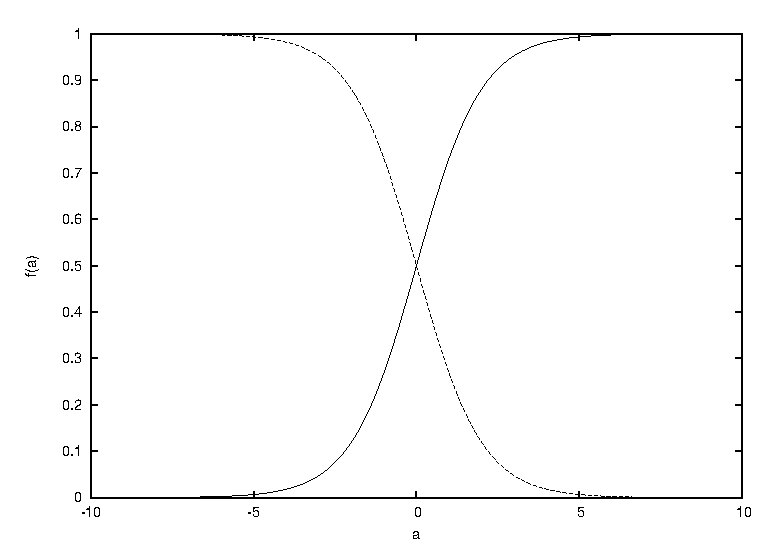
\includegraphics[scale=0.65]{img/ssigmoid.eps}
\caption{\figfont anti-simmetria della funzione sigmoide}\label{fig:ssigmoid}
\end{figure}
Il valore $ a $ pu� essere pensato come composizione: $ a = sign(a)\cdot\vert a\vert $. In relazione al segno di $ a $, si pu� notare che il grafico della funzione sigmoide � perfettamente anti-simmetrico, come riportato in figura \ref{fig:ssigmoid}, e cos� anche quello della funzione segno. Ci� significa semplicemente che: $g(-a) = 1 - g(a) $. Questo � un buon punto di partenza per riuscire a proteggere l'informazione sul segno di $ a $, o almeno per fare un tentativo in questa direzione.\\
Con questi presupposti, Bob pu� scegliere in maniera del tutto casuale di cambiare il segno ad $ a $ prima di inviare il valore ad Alice, anche grazie alle propriet� omomorfiche del cifrario. Semplicemente, basta notare che: $ E(a)^{-1} = E(-a) $, dove $ E(x) $ rappresenta il valore ottenuto dalla cifratura di $ x $. Cos� facendo Alice pu� decifrare ed elaborare i dati come di consueto, per� ci� che restituir� a Bob non sar� pi� la cifratura di $ g(a) $ ma bens� quella di $ g(-a) $, ovvero $ E(g(-a)) $. A questo punto, sempre in base alle propriet� sia della funzione sigmoide che del cifrario utilizzato, Bob potr� recuperare ci� a cui � interessato effettuando semplicemente una sottrazione, infatti:
$$ E(g(a)) = E(1 - g(-a)) = E(1)E(g(a))^{-1} $$
In questo modo le idee di Alice sono un po' pi� confuse ed ella non sa quale neurone � realmente attivo o meno. Del resto, questa intuizione � applicabile solamente alle funzioni segno e sigmoide, ma non vale in generale per qualsiasi funzione. Ci� nonostante, proprio queste due funzioni sono quelle coinvolte nel protocollo proposto e, laddove vi sia la necessit� di operare con altre funzioni, esister� allo stesso modo il bisogno di concepire nuove metodologie di occultamento. In ogni caso, nell'ambito delle reti neurali le funzioni pi� largamente utilizzate per il calcolo del valore di attivazione sono proprio la funzione segno e la funzione sigmoide che, come indicato, si prestano alle tecniche di cui sopra.
\paragraph{Occultamento della rete neurale.}
Un altro aspetto da proteggere � la topologia della rete, ovvero il numero di neuroni presenti e il modo in cui questi sono connessi fra loro. Intuitivamente, ci� � applicabile solamente ai livelli intermedi in quanto non avrebbe senso voler nascondere numero e disposizione dei neuroni di ingresso o di uscita.\\
L'idea alla base dell'occultamento della struttura di una rete neurale consiste nell'inserire tale oggetto all'interno di una rete composta da $ L $ livelli e $ M_i $ nodi per ciascun livello, dove ovviamente sia $ \sum_iM_i > N $, con $ N $ numero di nodi della rete originale. In questo modo vengono aggiunti $ \sum_iM_i - N $ neuroni fittizi, del tutto somiglianti ai neuroni originali, connessi con questi tramite collegamenti in ingresso dal peso casuale ma senza alcun collegamento in uscita diretto ai neuroni della rete incapsulata. Cos� facendo, i neuroni fittizi non influenzeranno in alcuno modo il comportamento originale della rete neurale. Ovviamente, comportandosi come neuroni reali ed essendo soggetti alle stesse leggi, anch'essi riceveranno collegamenti in ingresso solo dai nodi appartenenti a livelli precedenti e proporranno collegamenti in uscita solo verso nodi (in questo caso esclusivamente fittizi) appartenenti a livelli successivi.\\
In questo modo Alice riuscir� ad ottenere solo un limite superiori $ \sum_iM_i $ del numero di nodi reale $ N $ e non riuscir� a capire il modo in cui questi sono connessi o, ancora, i pesi associati alle connessioni. Inoltre, $ L $ indica anche un limite riguardo alla lunghezza del percorso presente fra i nodi di ingresso e quelli di uscita. Un incremento dei valori $ L $ e $ M_i $ protegger� meglio la topologia della rete, ma non bisogna trascurare in questo caso anche il fatto che ci� incide in maniere notevole sulle prestazioni, aumentando di fatto il carico computazionale e il numero di interazioni fra le parti.
\paragraph{Permutazione.}
L'unica cosa rimasta realmente da proteggere � il valore di $ \vert a\vert$, che rischia di essere rivelato, insieme al peso associato ai collegamenti, dall'applicazione ripetuta del protocollo da parte di Alice, come evidenziato in sezione \ref{sec:aim}. Ovviamente, questa � una situazione potenzialmente pericolosa e bisognerebbe possibilmente evitarla.\\
La soluzione proposta � quella di permutare la posizione dei singoli neuroni all'interno di un livello. Infatti, basandosi sulle propriet� delle reti feed-forward, � dimostrabile che questa operazione non influisce in alcun modo sul risultato finale. Bisogna sottolineare che le permutazioni valide possibili sono solamente quelle che mantengono la posizione in termini di livello di appartenenza del nodo. Anche in questo caso, agendo sui parametri citati si incrementa il numero di possibili differenti permutazioni valide ma, di contro, anche la complessit� computazionale dell'intero processo.\\
Come spesso accade, la sicurezza ha un prezzo in termini di tempo di calcolo e risorse utilizzate per il suo conseguimento.
\paragraph{}
Finite le dovute osservazioni sui vari aspetti coinvolti nell'algoritmo relativo alle reti neurali multi-livello, � possibile presentare finalmente la soluzione proposta nel protocollo commentandola passo dopo passo. Ovviamente, prima di tutto Bob dovr� inglobare la rete neurale in un involucro che risulti valido secondo le caratteristiche descritte nel paragrafo precedente, con $ L $ e $ M_i $ fissati; in altri termini, Bob dovr� espandere la rete aggiungendo in essa un determinato numero di nodi fittizi per ogni specifico livello. Inoltre, Bob dovr� accordarsi con Alice su alcuni valori: il parametro di quantizzazione $ Q $ (di cui si rimanda la spiegazione alla sezione \ref{sec:wwni}) e un parametro $ s $ da usare con il cifrario. Inoltre, Alice dovr� generare una coppia di chiavi pubblica/privata (inviando la prima a Bob), mentre Bob dovr� permutare per ogni singolo livello le posizioni dei nodi componenti la rete neurale.\\
Si osservi che nel protocollo seguente tutti i neuroni (reali e fittizi) vengono trattati allo stesso modo, dato che non vi sono effettivamente differenze (almeno dal punto di vista di Alice). Ci� nonostante, bisogna ricordare che i valori di uscita dei nodi fittizi non saranno in realt� utilizzati se non come valori di ingresso per altri nodi fittizi. Inoltre, si suppone che a seguito dell'occultamento della rete Bob sia comunque sempre in grado di generare il vettore $ \bar{x}_j $ contenente i valori di ingresso per ogni singolo neurone, ovvero a partire da un dato neurone $ k $ Bob sar� sempre in grado di ricostruire il vettore $ \bar{x}_j $ contenente i nodi che presentano collegamenti in uscita diretti al neurone $ k $ in questione.\\
Il vettore dei valori di ingresso fornito da Alice sar� chiamato $ \bar{c} $, mentre il vettore dei pesi sar� detto $ \bar{w}_j^{(i)} $ dove sia $ i = 1,\; \ldots,\; L $ e $ j = 1,\; \ldots,\; M_i $.
\begin{itemize}
\item Per ogni $ i = 1,\; \ldots,\; L $ e per ogni $ j = 1,\; \ldots,\; M_i $, ovvero per ogni nodo intermedio, vengono effettuati i passi sotto elencati.
\begin{itemize}
\item Bob calcola il valore $ d = E(a) $, come spiegato in sezione \ref{subsec:cip}, che risulta essere (una volta in chiaro) la somma pesata dei valori in ingresso al nodo
\item Bob calcola in maniera casuale $ t_j \in \lbrace-1, 1\rbrace $, se $ t_j = -1 $ allora viene calcolato $ d = d^{-1} $
\item Bob invia ad Alice il valore $ d $, che sar� decifrato ottenendo il valore $ a $, elaborato secondo una determinata funzione $ g $ ottenendo $ g(a) $ e quindi cifrato nuovamente nella forma $ z = E(g(a)) $ per essere restituito al mittente
\item Se in precedenza era stato calcolato $ t_j = -1 $, allora viene posto $ z = E(1)z^{-1} $
\end{itemize}
\item Per ogni $ k = 1,\; \ldots,\; O $, con $ O $ numero di neuroni di uscita, vengono effettuati i passi sotto elencati.
\begin{itemize}
\item Bob computa il valore $ d = E(a) $, come discusso in sezione \ref{subsec:cip}
\item Bob invia il valore $ d $ ad Alice
\item Alice decifra $ d $ ottenendo il valore $ a $ e calcola localmente il risultato $ g(a) $, ricavando cos� il valore del determinato nodo di uscita, dove sia $ g $ la funzione di attivazione associata allo specifico nodo
\end{itemize}
\end{itemize}

\section{Possibili applicazioni}
Il protocollo proposto � interessante se inquadrato all'interno di determinate situazioni in cui un suo utilizzo potrebbe, effettivamente, riservare un grado di sicurezza tanto a chi sfrutta il servizio quanto a chi lo offre.\\
Per fare un esempio, si pensi allo scenario in cui un noto ospedale decida di investire nella creazione, addestramento e quindi offerta di reti neurali in grado di classificare un paziente a partire da determinati sintomi (sottomessi come ingressi del sistema). Ovviamente, dal punto di vista dell'ospedale c'� un forte interesse nel proteggere il proprio investimento in quanto si suppone siano spesi soldi e denaro per ottenere il prodotto finale. L'aspetto pi� importante per� � il punto di vista dell'utente del servizio: quest'ultimo, infatti, potrebbe non voler mettere a conoscenza di nessuno i sintomi che lo hanno spinto ad usufruire del servizio messo a disposizione dall'ospedale e, plausibilmente, tantomeno vorr� far sapere a chiunque il suo stato di salute. Se ci� non � del tutto chiaro nell'ottica di un normale cittadino, si pensi al caso in cui ad usufruire del servizio siano personaggi noti appartenenti per esempio al mondo della politica. Sapere che uno specifico soggetto che ricopre cariche di uno determinato livello ha o meno una malattia di una certa gravit� pu� influire non poco sull'ambiente che lo circonda.\\
Quello proposto � solo uno dei tanti casi in cui la possibilit� di operare in dominio cifrato da parte di una rete neurale si rivela utile per molti aspetti. Basta avere un po' di fantasia per trovare tante altre applicazioni al protocollo descritto. Questa � infatti la logica conseguenza della necessit� crescente, al giorno d'oggi, nel conseguire principi di sicurezza sui dati scambiati fra soggetti, che si sposa con una tecnologia gi� affermata come le reti neurali e la loro ormai nota capacit� di classificazione.

\section{Lavorare con valori non interi}\label{sec:wwni}
Un risvolto negativo nell'uso all'interno di un protocollo di un sistema crittografico qualsiasi � dato dal fatto che questo funziona solamente con valori interi di dimensione arbitraria. � necessario quindi un metodo per riuscire ad operare con numeri reali.\\
Prima di tutto � possibile rappresentare in maniera classica i numeri positivi in $ \lbrace 0,\; \ldots,\; \frac{n^s - 1}{2}\rbrace $ e quelli negativi in $ \lbrace \frac{n^s - 1}{2} + 1,\; \ldots,\; n^s - 1\rbrace $, dove sia: $ -1 = n^s - 1 $. Quindi, dato un valore reale $ x \in \mathbb{R} $, � possibile quantizzarlo con un fattore $ Q $ e approssimarlo a $ \tilde{x} = \lfloor\frac{x}{Q}\rfloor \sim \frac{x}{Q} $, valida per quantizzazioni sufficientemente fini.\\
Ovviamente, valgono ancora le propriet� omomorfiche del cifrario, ovvero:
$$ D(E(\tilde{x}_1)\cdot E(\tilde{x}_2)) = \tilde{x}_1 + \tilde{x}_2 \sim \frac{x_1 + x_2}{Q} $$
Questo mette in condizioni Bob di effettuare un numero arbitrario di somme in dominio cifrato. Inoltre, anche la seconda propriet� � ancora valida, sebbene abbia un rovescio della medaglia da non trascurare. Infatti:
$$ D(E(\tilde{x})^{\tilde{a}}) = \tilde{a}\cdot\tilde{x} \sim \frac{a\cdot x}{Q^2} $$
La presenza del fattore $ Q^2 $ comporta che da un lato la dimensione dei numeri cifrati cresca in maniera esponenziale con il numero delle moltiplicazioni effettuate, mentre dall'altro lato Bob deve rivelare ad Alice il numero di moltiplicazioni cos� che possa compensare la presenza del fattore $ Q^2 $. Fortunatamente, nel primo caso il cifrario sopperisce al problema grazie alla possibilit� di incrementare il parametro $ s $ per poter cifrare numeri pi� grandi. Nel secondo caso, bisogna osservare che nel protocollo � effettuata una sola moltiplicazione per ogni elemento cifrato e quindi non ci sono perdite sulla sicurezza in quanto Bob non deve rivelare a priori niente ad Alice (anch'essa sa gi� il numero effettivo di moltiplicazioni effettuate).\\
La soluzione al primo problema consiste nello scegliere il parametro $ s $ in modo che il valore contenuto nel testo cifrato dopo la computazione risulti minore di $ n^s $. Posto $ X $ il limite superiore della norma relativa al vettore di valori in ingresso fornito da Alice e sia $ W $ il limite superiore della norma relativa al vettore dei pesi sui collegamenti nella rete neurale, ogni prodotto scalare calcolato all'interno del protocollo � limitato da $\vert x\vert\vert w\vert \cos{\hat{xw}} \leq XW $. Dato un modulo $ n $ sufficientemente grande per scopi di sicurezza, � possibile selezionare un parametro $ s $ cos� che:
$$ s \geq \lceil \log_n{\frac{2XW}{Q^2}}\rceil $$
Dove il 2 � dovuto alla presenza di valori sia negativi che positivi. Cos� facendo, si riesce ad ottenere (seppure con qualche limitazione) un cifrario capace di operare con numeri reali adeguatamente quantizzati e quindi riportati in un intervallo di interi positivi.

Ovviamente, la possibilit� di trattare i numeri reali all'interno del protocollo si ripercuote su chi propone la rete neurale in termini di scelta del corretto valore utilizzato per quantizzare tali numeri. Infatti, se da un lato un valore di quantizzazione troppo piccolo rischia di trascurare alcune cifre decimali e falsare il risultato, dall'altro lato un valore di quantizzazione troppo grande appesantisce la computazione e porta ad un accrescimento della complessit�.\\
Pertanto, bisogna porre molta attenzione alla scelta del fattore di quantizzazione e assicurarsi che esso non influisca n� sul risultato n� sul tempo necessario per conseguirlo, ma piuttosto rappresenti un giusto compromesso in grado di sposare le esigenze degli utenti con la loro pazienza.

\chapter{NNSec}\label{cap:two}
\epigraph{Se ascolto dimentico, se osservo ricordo, se faccio imparo}{Baden Powell}

NNSec, o Neural Network Secure, � un applicativo scritto totalmente in Java che implementa il protocollo precedentemente descritto, lasciando all'utente diversi gradi di libert� nella configurazione lato server.

Nello sviluppo di NNSec sono state introdotte molte tecniche prese in prestito dai pi� svariati ambiti della programmazione, come ad esempio metodologie mirate per la gestione dell'accesso concorrente (spesso presenti nell'ambito dei sistemi operativi) applicate alla singola rete neurale, o pattern di progettazione tipici dell'ingegneria del software come il pattern factory o il pattern composite, utilizzati per risolvere in modo elegante e pulito alcuni problemi cruciali del progetto.

Basandosi interamente su Java, NNSec fa uso e abuso di molti degli strumenti che questo linguaggio offre allo sviluppatore. In particolare, come sar� illustrato e discusso in seguito, articola gran parte della sua struttura su RMI (o Remote Method Invocation) e si appoggia alle Java Swing per poter fornire una GUI piacevole ed efficace all'utente finale. Ci� nonostante, sono stati usati anche strumenti esterni non direttamente forniti insieme alla libreria standard di Java, come ad esempio un tool per la progettazione, lo sviluppo e la creazione di un parser in modo automatico.

Il risultato finale del lavoro di tesi � rappresentato proprio dal programma NNSec, ovvero dalla realizzazione di uno strumento che permettesse di toccare con mano il protocollo proposto e fino ad oggi discusso solamente in linea teorica. Pertanto, data l'importanza non trascurabile dei dettagli tecnici che stanno dietro al cosa e permettono di capire il come, saranno discussi in questo capitolo i principi di progettazione e le linee guida adottate durante la realizzazione del software.

\newpage

\section{Progettazione e Struttura}\label{sec:ps}
\begin{figure}
\centering
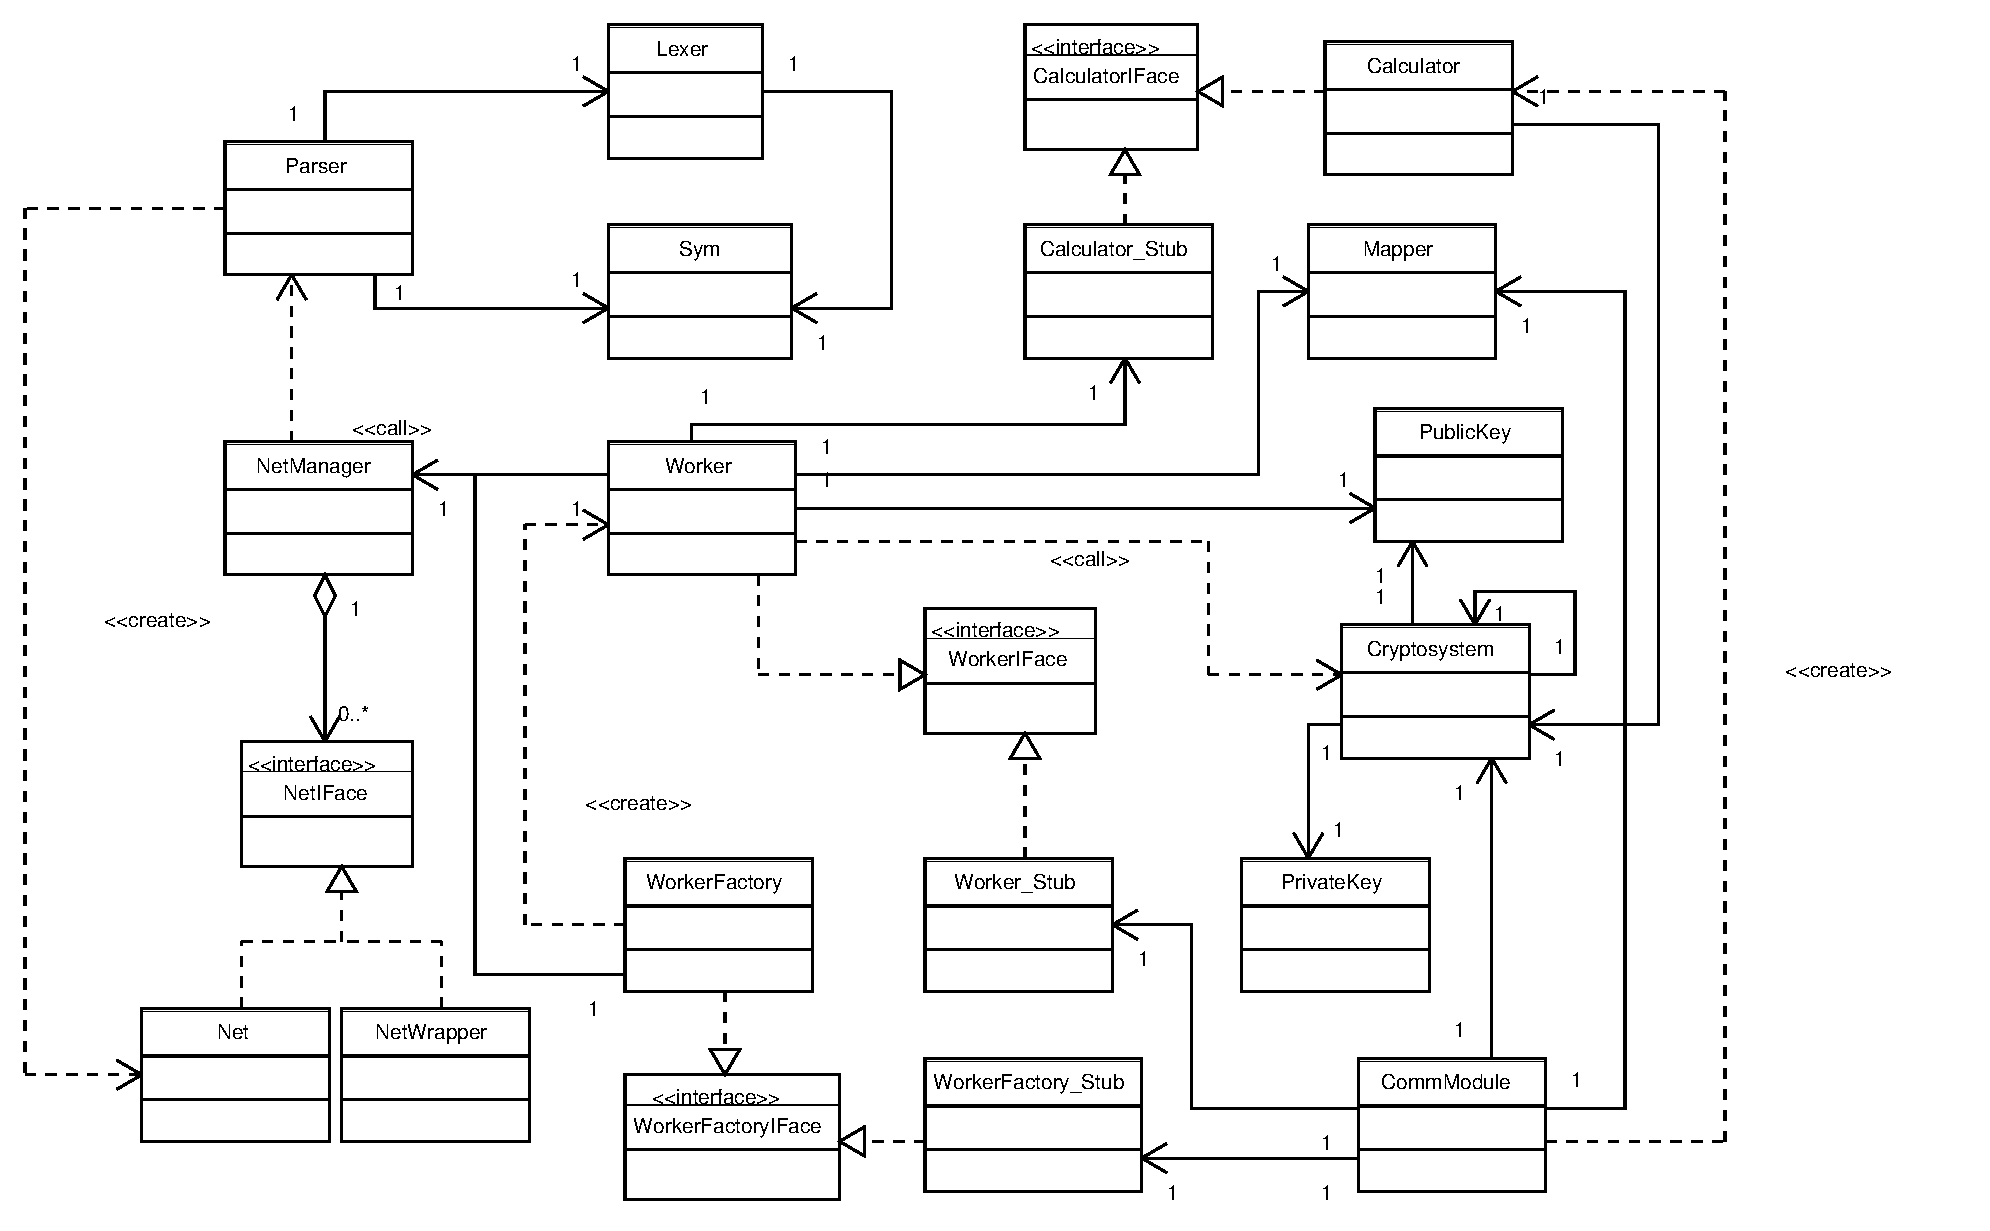
\includegraphics[scale=0.60,angle=90]{img/classdiag.eps}
\caption{\figfont diagramma delle classi (semplificato)}\label{fig:cdiag}
\end{figure}
NNSec nasce come implementazione del protocollo descritto nel capitolo precedente, con lo scopo di trasformarlo in qualcosa di concreto su cui poter effettuare i primi esperimenti e da utilizzare come base per sviluppi futuri. NNSec rappresenta, quindi, un banco di prova per la crittografia in questo ambito da cui poter attingere cos� da ricavare dati importanti per valutazioni e progetti in questa direzione.

Va detto fin da subito che proprio nel tentativo di rendere agevoli modifiche, estensioni o studi a posteriori del software, tutti i file sono stati documentati con commenti estraibili in formato html tramite l'uso di javadoc. Inoltre, l'insieme delle classi � stato progettato in modo da poter rendere non traumatiche eventuali variazioni nel codice, cos� da non dover costringere alla modifica di tutti i file per poter cambiare anche di poco un algoritmo o una interfaccia a causa di dipendenze pesanti.\\
La struttura di NNSec, seppure non esagerata in numero di classi, risulta abbastanza complessa in quanto sono state introdotte alcune metodologie proprie dell'ingegneria del software, come il pattern singleton ma non solo, sono state sfruttate alcune tecniche particolari messe a disposizione dal linguaggio Java, come le classi interne e il loro retro-riferimento verso l'esterno, e sono state ampiamente utilizzate tecnologie specifiche di questo linguaggio e della sua libreria, come RMI, che rendono pi� ostica la comprensione delle relazioni fra gli oggetti e la stesura di un diagramma delle classi che sia al tempo stesso completo e chiaro. Una versione semplificata di quest'ultimo � comunque riportata in figura \ref{fig:cdiag}.

I principi adottati durante l'intera ideazione delle classi sono quelli del disaccoppiamento fra di esse (cos� da abbattere le inter-relazioni che si possono venire a creare fra oggetti altrimenti indipendenti) e la divisione dei compiti in componenti elementari. Nello specifico, ogni classe � stata creata tenendo salda in mente la regola base della programmazione, anche detta KISS\footnote{Keep It Simple, Stupid (Rendilo semplice, banale)}: questo principio invita a non progettare pensando fin da subito alle possibili ottimizzazioni applicabili in un punto piuttosto che un altro, ma cercando di mantenere uno stile di programmazione che miri alla semplicit� ed eviti la complessit�, lasciando eventuali ottimizzazioni al compilatore o alle successive fasi di sviluppo. Questo ha portato ad un insieme di classi forse pi� ampio del necessario ma in cui ognuna � rappresentata da poche centinaia di righe di codice (ben documentato nei particolari), in alcuni casi addirittura solo alcune decine. Classi semplici, quindi, ma funzionali, ognuna relegata a svolgere un compito preciso, ben definito e senza doversi caricare di un numero esagerato di operazioni.\\
Per quanto riguarda le relazioni fra classi diverse, queste sono state mantenute al minimo cercando di creare dei punti di accesso specifici su cui ognuna potesse contare per l'interazione con le altre. Tutto ci�, ovviamente, rappresenta una specie di contratto che il programmatore non dovr� infrangere neanche al momento in cui si trover� a dover stravolgere completamente la struttura interna di una delle classi coinvolte. Baster�, pertanto, lasciare intatti i punti di contatto che queste offrono verso l'esterno ed eventuali modifiche non si ripercuoteranno in alcun modo verso l'esterno.\\
Un discorso simile a quanto appena esposto � applicabile anche alle interfacce, ampiamente usate soprattutto a causa della forzatura imposta dall'uso di RMI che obbliga ad appoggiare ogni classe su una specifica interfaccia (che sar�, poi, quella esportata remotamente). Nella progettazione di queste interfacce si � cercato di definire in modo chiaro e completo il numero e il prototipo dei metodi esposti, in quanto questi rappresentano anche le possibili chiamate effettuabili da parte di oggetti remoti. Vale la stessa osservazione fatta anche in precedenza: queste interfacce rappresentano un accordo fra chi espone i metodi e chi tali metodi li sfrutta. Stravolgere la loro struttura significherebbe costringere alla re-implementazione di un gran numero di classi, cosa solitamente non troppo gradita. Anche per questo � stata riposta un'attenzione particolare nella progettazione delle interfacce remote, cos� da lasciare ampio spazio ad una totale riscrittura dei metodi nel caso in cui nuovi algoritmi prendano il posto degli attuali ma senza che questo comporti un terremoto all'interno del codice con conseguente modifica di gran parte di esso.
\paragraph{}
Alcune note vanno fatte sul risultato finale, ovvero il software NNSec.\\
A seguito di svariate scelte di progetto a monte della fase di sviluppo e in corso d'opera, NNSec gode di alcune caratteristiche particolari non necessarie ma senza ombra di dubbio desiderabili:
\begin{itemize}
\item la componente server NNSec supporta l'interazione con pi� client contemporaneamente, riuscendo a servire pi� richieste in modo concorrente e regolando l'accesso alle risorse per un corretto uso di quest'ultime che garantisca l'integrit� dei dati
\item all'interno di NNSec sia i percettroni che le reti neurali multi-livello feed-forward sono rappresentate astraendo dal loro tipo effettivo, permettendo la memorizzazione e gestione con funzioni e  strutture dati generiche e non specifiche a seconda della tipologia di oggetto
\item gli algoritmi proposti in linea teorica nel protocollo (si veda a tale proposito sezione \ref{sec:proto}) sono stati uniformati in un unico algoritmo capace di interagire e trattare correttamente sia percettroni che reti neurali multi-livello feed-forward
\end{itemize}
Il tutto sfocia in un programma pi� semplice e pi� efficiente in grado di gestire l'accesso concorrente alle risorse (ovvero, alle reti neurali messe a disposizione per l'uso remoto), tanto facile da gestire quanto da capire e che generalizza in molti punti anzich� articolarsi in rami diversi facendo distinzioni a monte sugli elementi trattati.

\section{NNSec}
Fedele alle linee guida di Java, anche NNSec � stato progettato assegnando ogni singola classe ad un package appropriato e suddividendo il progetto in un insieme articolato ma coerente di subpackage, cos� da permettere a chi fosse interessato di orientarsi senza difficolt� fra le classi coinvolte.

L'insieme delle classi componenti NNSec � stato partizionato in cinque gruppi principali, ovvero le classi che compongono il parser, il cifrario, tutti gli elementi coinvolti nella realizzazione e gestione delle reti neurali, le classi lato server e quelle lato client, rispettivamente appartenenti ai subpackage \texttt{parser}, \texttt{cryptosystem}, \texttt{net}, \texttt{server} e \texttt{client}. Questa suddivisione � stata utile anche per separare in linea teorica le classi fra loro, in modo da poter attribuire velocemente un ruolo univoco in uno specifico ambiente ad ognuna di esse. Ci� nonostante, per motivi dovuti tanto all'uso di RMI quanto alla struttura del protocollo, la componente server si avvale anche di classi e interfacce presenti in \texttt{nnsec.client}, cos� come la componente client si affida a classi e interfacce in \texttt{nnsec.server}; entrambe, inoltre, attingono da tutti gli altri sotto pacchetti presenti nel package \texttt{nnsec}. La suddivisione, pertanto, sebbene marcata in modo netto nasconde fra le righe relazioni inter-pacchetto che rendono l'insieme delle classi e delle interfacce un'entit� unica ben amalgamata.\\
Il package \texttt{nnsec} rappresenta il package principale del progetto. In realt�, questo package � fittizio e non contiene classi ma fa da involucro per i subpackage sopra elencati, raccogliendoli in un insieme unico. Non � pertanto di particolare interesse e non sar� discusso ulteriormente.

\section{Parser}
Il subpackage \texttt{parser} � il package che contiene le classi relative all'interprete dei file di ingresso per la descrizione delle reti neurali in NNSec.

Il ruolo del parser risulta essere abbastanza importante anche se non direttamente coinvolto nell'implementazione del protocollo proposto. Infatti, il protocollo tratta l'uso di reti neurali remote in sicurezza e queste, in un modo o nell'altro, devono essere create e addestrate ma soprattutto rese disponibili dentro a NNSec, lato server. In quest'ottica entra in gioco il parser e un linguaggio definito ad hoc per descrivere le reti stesse, comprensibile da NNSec. Ci� nonostante, il compito di creare e allenare le reti non riguarda NNSec e non sar� pertanto approfondita, discussa o analizzata alcuna tecnica in questo senso.\\
L'utilit� del parser, oltre a quella di poter descrivere le reti neurali in una forma ad alto livello semplice e comprensibile, risiede anche nella capacit� intrinseca (se adeguatamente inserito nel sistema) di poter caricare nuove reti neurali a caldo, il che permette di non dover fermare il server in alcun caso per effettuare operazioni del genere. Questo, seppure in molti casi sia dato per scontato, rappresenta comunque un'interessante e utile caratteristica.

\subsection{Grammatica dei file in ingresso}
Essendo NNSec un programma che mira ad utilizzare reti neurali ma trattandole indirettamente (ovvero, senza crearle o addestrarle, ma usando piuttosto il risultato finale di un processo gi� terminato a monte), la grammatica dei file di descrizione delle reti neurali avrebbe potuto basarsi su un formato di file gi� esistente. Ci� nonostante, � stata sviluppata una grammatica ad-hoc per NNSec a causa dei seguenti motivi:
\begin{itemize}
\item ogni programma candidato che proponga un proprio formato di file per la descrizione delle reti neurali non separa la descrizione della struttura relativa alla rete neurale da tutta una serie di parametri legati al programma stesso
\item sfruttare una grammatica creata per altri scopi costringe allo sviluppo di un parser pi� complesso capace di analizzare file contenenti dati che saranno scartati in buona percentuale e portando probabilmente a piegarsi a grammatiche scomode e poco flessibili
\item basarsi su un formato proprio di un altro software crea una dipendenza da tale strumento che potrebbe rappresentare una nota stonata col tempo e costringe l'utente a familiarizzare con tale programma, privandolo della libert� di scelta riguardo al come preparare le proprie reti neurali
\end{itemize}
Pertanto, NNSec � accompagnato da una grammatica (riportata in appendice) pensata appositamente per questo scopo, al tempo stesso semplice e intuitiva, cos� da permettere a chiunque di scrivere file di descrizione per reti neurali, ma anche completa e flessibile, in modo da lasciare spazio a virtuosismi e tecniche avanzate senza trascurare la possibilit� di un ampliamento futuro che non dovesse per forza costringere alla riscrittura di tutti i file gi� esistenti per le reti neurali.\\
La possibilit� di creare veri e propri traduttori da un formato come quello proposto da altri programmi al formato di ingresso per NNSec rimane sempre una strada percorribile e rende praticamente possibile l'uso di qualsiasi programma di creazione e allenamento per le reti neurali, a patto che poi si riesca a convertire i file da un formato all'altro (a mano o tramite strumenti automatici), cosa che per altro non richiede particolari abilit� o conoscenza della materia. Questa � anche la strada seguita nella preparazione di reti neurali per effettuare alcuni test con NNSec, create e allenate con il tool JavaNNS (prelevabile da \cite{javanns}) e convertite nel formato comprensibile da NNSec tramite una serie di appositi script.

\subsection{JFlex e JavaCUP}
La creazione di una coppia di analizzatori lessicale e sintattico, utili per poter estrapolare potenziali elementi grammaticali da un flusso in ingresso e poterli valutare in quest'ottica decretandone l'appartenenza ad uno specifico linguaggio o meno, � un lavoro abbastanza arduo. Per quanto ci si possa sforzare, � piuttosto difficile ottenere un prodotto finale che sia efficiente anche se apparentemente perfettamente funzionante. Meglio affidarsi a strumenti automatici che, a partire da una collezione di simboli e la descrizione di una grammatica basata su di questi, producano un interprete tanto efficace quanto efficiente in pochi istanti, risparmiando non poca fatica agli sviluppatori.

In quest'ottica, anche nello sviluppo di NNSec � stato ceduto il passo all'uso di due software open-source molto utilizzati proprio per questo scopo: JFlex e JavaCUP. I due software citati sono reperibili dal web a partire da \cite{jflex} e \cite{javacup}.\\
Il primo dei due strumenti, JFlex, � utilizzato per la realizzazione di una classe in grado di spezzare un determinato flusso di ingresso in una serie di elementi predefiniti, specificati a priori, e di individuare i casi in cui vi siano oggetti non appartenenti a questo insieme. In questo modo, associando ad ogni elemento per esempio un identificativo numerico, si pu� pensare di dividere un ipotetico flusso continuo di caratteri in elementi atomici, rappresentandolo su di un flusso di valori interi pi� facilmente trattabile a valle del processo di suddivisione. Questa idea sfrutta il principio di \textit{divide et impera}, caro anche a molti altri algoritmi come quelli di ordinamento, per cui si separa il compito di interpretazione dei dati in ingresso da quello di valutazione riguardo alla correttezza sintattica di tali dati. L'oggetto prodotto da JFlex ha il compito di svolgere la prima delle due funzioni.\\
Per quanto riguarda JavaCUP, invece, esso ha il compito, basandosi sempre sullo stesso insieme di elementi predefiniti, di determinare come gi� anticipato la validit� sintattica del flusso di elementi estratti dall'insieme di dati e l'appartenenza o meno di tale struttura di informazioni ad un linguaggio desiderato. Lavorando ad esempio su valori interi, ognuno corrispondente ad un determinato simbolo, il compito di questo oggetto � molto semplificato e lascia ampio spazio ad ottimizzazioni tramite l'uso di tabelle e speciali algoritmi concepiti proprio a questo scopo. La teoria che sta dietro al funzionamento di un parser e tutto ci� che � legato alle grammatiche e i linguaggi regolari esula dallo scopo di questa tesi e le classi realizzate, seppure funzionali allo scopo, sono molto semplici e in grado di interpretare un linguaggio a sua volta di facile comprensione e analisi.

\section{Cryptosystem}
Il subpackage \texttt{cryptosystem} contiene principalmente le classi fondamentali per quanto riguarda le sessioni di cifratura/decifratura, la quantizzazione e la mappatura dei valori reali, cos� da permettere al resto del sistema di usufruire di questi servizi in modo trasparente e senza sporcare il codice restante. In questo package sono presenti un insieme di classi che implementano il cifrario, analizzato in sezione \ref{subsec:cip}, e permettono di operare facilmente con valori reali, come discusso in sezione \ref{sec:wwni}.

Separare tanto le operazioni relative alla cifratura/decifratura dei messaggi quanto quelle relative alla gestione dei valori reali (quantizzati e rappresentati all'interno di un arco di valori interi positivi), permette di sviluppare nel resto del programma un codice pi� snello e pulito, che si appoggia a queste primitive senza implementare al suo interno alcuna operazione orientata in tal senso (se non le semplici chiamate di metodi e la creazione degli oggetti dovuti). Mettendo a disposizione uno strato come quello proposto, vengono messi sia i programmatori che gli studiosi interessati al codice in condizione di operare in un ambiente in cui cifrare o validare un valore consiste in una semplice invocazione di un metodo, come se queste operazioni fossero native e integrate nell'ambiente stesso.

\subsection{Numeri primi, chiavi pubbliche/private e BigInteger}\label{subsec:bigkey}
Prima di procedere con la descrizione del cifrario � utile ripassare alcuni concetti e inquadrare aspetti provenienti dalla teoria in uno scenario pratico. Per ulteriori approfondimenti si faccia riferimento a \cite{goldreich2001fcb} e \cite{goldreich2004fci}.

Una delle nuove frontiere della crittografia � rappresentata dalla crittografia asimmetrica, anche detta a chiave pubblica/privata. Supponendo che Bob e Alice vogliano scambiarsi dati in sicurezza, ad ognuno di loro � demandata la generazione di una coppia di chiavi pubblica e privata di cui:
\begin{itemize}
\item la chiave privata � segreta e viene utilizzata per decifrare i dati
\item la chiave pubblica viene distribuita alla controparte e utilizzata quindi per cifrare i dati
\end{itemize}
Supponendo che Alice voglia inviare un messaggio, dovr� cifrarlo con la chiave pubblica di Bob il quale potr� decifrarlo con la propria chiave privata. In alcun caso si potr� usare una stessa chiave per le due fasi, ovvero non si potr� decifrare con la stessa chiave con cui � avvenuta la cifratura.\\
Le chiavi pubbliche e private sono in molti casi generate a partire da una coppia di numeri primi $ p $ e $ q $ molto grandi, scelti a caso l'uno indipendentemente dall'altro e quindi elaborati in un qualche modo differente a seconda del cifrario. Ad esempio, a partire dai valori di cui sopra in RSA:
\begin{itemize}
\item si calcola il loro prodotto $ n $, chiamato modulo (dato che tutta l'aritmetica seguente � modulo $ n $)
\item si sceglie un numero $ e $, tale che sia coprimo con $ (p-1)(q-1) $; ovvero, si sceglie $ e $ tale che il massimo comune divisore fra $ e $ e $ (p-1)(q-1) $ sia $ 1 $.
\item si calcola un numero $ d $ tale che: $$ e\cdot d\; (mod\; (p-1)(q-1)) \equiv 1 $$
\end{itemize}
La chiave pubblica � rappresentata dalla coppia $ (n, e) $, mentre la chiave privata � data dalla coppia $ (n, d) $. La forza di RSA risiede nel fatto che fattorizzare il valore $ n $ nel tentativo di risalire ai due numeri primi che lo hanno generato � computazionalmente molto difficile soprattutto se $ n $ � molto grande.

I principali problemi di questi protocolli risiedono nella difficolt� di generazione di numeri pseudo-casuali e di numeri primi molto grandi.\\
Nel primo caso, esistono algoritmi in grado di generare una successione di numeri i cui elementi sono approssimativamente indipendenti l'uno dall'altro, anche se non tutti sono utilizzabili in crittografia. Un possibile esempio � dato dall'algoritmo BBS, o Blum Blum Shub (discusso in \cite{blumblumshub}).\\
Nel secondo caso, bisogna osservare che non esistono ad oggi algoritmi in grado di determinare con estrema certezza se un dato numero � primo o meno ed esistono alcuni numeri che presentano tutte le caratteristiche proprie dei numeri primi pur non essendo tali. Questo si ripercuote nella possibilit� di incappare in numeri solo apparentemente primi e quindi si corre il rischio di essere in possesso di una coppia di chiavi fragile. Ci� nonostante, esistono metodi per effettuare un test di primalit� per un numero come l'algoritmo di Miller-Rabin (di cui � data una trattazione completa in \cite{millerrabin}, dove sono analizzate anche le problematiche accennate poco sopra).

\paragraph{La soluzione BigInteger.}
Il linguaggio Java mette a disposizione la classe \texttt{BigInteger}\footnote{http://java.sun.com/j2se/1.5.0/docs/api/java/math/BigInteger.html} per risolvere in maniera comoda il problema e sollevare il programmatore dallo sviluppo di algoritmi mirati. Questa classe si basa proprio sul test di primalit� di Miller-Rabin e permette di creare numeri primi per cui:
\begin{itemize}
\item � possibile definire una lunghezza in numero di bit, detta \textit{bitLength}, ottenendo cos� un numero primo compreso fra $ 0 $ e $ (2^{bitLength} - 1) $ inclusi
\item � possibile definire un livello di sicurezza detto \textit{certainty}, tale per cui la probabilit� che il numero ottenuto rappresenti un numero primo sia superiore a $ \left( 1 - \frac{1}{2^{certainty}}\right) $
\end{itemize}
Inoltre, la classe \texttt{BigInteger} (largamente usata in NNSec) propone tutta una serie di metodi per poter eseguire operazioni fra oggetti di questo tipo. Ad esempio, sono presenti metodi per effettuare divisioni e moltiplicazioni, somme e sottrazioni ma anche per ricavare il minimo comune divisore fra due \texttt{BigInteger}, effettuare operazioni di modulo o test di primalit� e tanto altro ancora.\\
Per approfondimenti sulla classe \texttt{BigInteger} si rimanda alla documentazione ufficiale del linguaggio Java.

\subsection{Il cifrario}
Analizzando la parte implementativa di NNSec e affrontando il concetto del cifrario preso in esame in sezione \ref{subsec:cip}, non sar� discusso come effettivamente funzionino o cosa si nasconda dietro alle primitive crittografiche (per una cui trattazione si rimanda a \cite{paillier} e \cite{brics}), ma piuttosto sar� aperta una parentesi su tutta una serie di tecniche messe a disposizione dal linguaggio Java e adottate nello sviluppo di questa classe.

Il cifrario infatti, rappresentato nella classe \texttt{Cryptosystem}, � uno degli elementi (anche se non l'unico) che basa la sua struttura sull'uso delle classi interne, o inner-class. Queste classi hanno alcune caratteristiche interessanti, brevemente riassunte in due punti: la loro capacit� di referenziare la classe contenitrice accedendo ai suoi metodi e le sue variabili (nota importante, anche se private) con la sola limitazione che esse devono essere definite come statiche e cos� anche i metodi acceduti se anche la classe interna lo �; la possibilit� di modificarne la visibilit� (o \textit{scope}), cos� che possano risultare a solo uso e consumo della classe che le contiene oppure accedibili anche dagli altri elementi del sistema (addirittura, se pubbliche e statiche possono essere istanziate e utilizzate da tutti gli altri oggetti nel sistema semplicemente attraverso la dicitura classe\_contenitrice.classe\_contenuta).\\
Combinando quindi la possibilit� di dichiarare una chiave privata come classe anch'essa privata interna al cifrario e la chiave pubblica come classe statica e a sua volta pubblica, con la capacit� di presentare metodi statici accedibili da chiunque senza essere obbligati ad istanziare un cifrario a s� stante, ecco che la funzionalit� completa � servita.\\
Infatti, ad Alice (che necessita di una coppia di chiavi pubblica e privata) baster� creare un nuovo cifrario che sar� utilizzabile senza difficolt� attraverso i metodi di interfaccia, sia per cifrare che per decifrare messaggi oltre che per esportare la chiave pubblica cos� da poterla dare ad altri soggetti (ovvero, a Bob). Per quanto riguarda Bob invece (che necessita solo di poter cifrare o decifrare messaggi, laddove possibile, tramite l'uso di una chiave pubblica fornita da Alice) anche in questo caso non esiste alcuna difficolt�: questo tipo di classe � accedibile per mezzo di metodi statici, senza essere obbligati a creare oggetti ex-novo sul proprio sistema se non ve ne fosse la necessit�. Questo significa che Bob, possedendo la sola chiave pubblica di Alice, non avr� necessit� di istanziare un nuovo cifrario per poterla utilizzare ma potr� usare tale chiave attraverso una serie di metodi statici della classe \texttt{Cryptosystem} che gli danno la possibilit� di elaborare i dati.

Questa classe dimostra quindi come sia possibile realizzare e strutturare elementi particolarmente complessi ma utili a risolvere svariati problemi in modo elegante e pulito, semplicemente sfruttando tutte quelle caratteristiche che un linguaggio come Java mette a disposizione e sono spesso trascurate o, peggio ancora, del tutto ignorate dagli sviluppatori.

Una nota particolare va fatta in merito a questa classe, ma prima bisogna aprire e chiudere velocemente una piccola parentesi. Uno degli anti-pattern pi� famosi e discussi perch� spesso seguito alla lettera (da notare che questi descrivono il modo sbagliato di fare le cose, quindi attenersi ad essi non � molto indicato) � detto \textit{Reinventare la ruota}. Molto brevemente, questo anti-pattern descrive il comportamento sbagliato di molti programmatori, i quali piuttosto che spendere poco del loro tempo a cercare qualcuno che abbia gi� affrontato (e risolto) il loro problema tendono ad impiegare molto del loro tempo riscrivendo da zero in modo fantasioso (e spesso di gran lunga meno efficiente) algoritmi, classi e funzioni di ogni tipo. In questo caso viene sfatato un po' questo mito e bisogna dire che la classe relativa al cifrario nasce come modifica (abbastanza ampia e profonda, a dire il vero) di un software giocattolo gi� pre-esistente fornito per testare l'algoritmo descritto e reperibile dalla rete Internet sulla pagina dello sviluppatore\footnote{http://www.daimi.au.dk/~jurik/research.html}.\\
� stata quindi seguita la via che prevede di adattare qualcosa di gi� esistente ai propri scopi, piuttosto che riprogettarlo da zero peccando di presunzione e rischiando di incappare in problemi di prestazioni.

\subsection{I numeri reali e la classe Mapper}
L'uso dei numeri reali come parametri di ingresso per reti neurali o come valori associati ai collegamenti fra i nodi che le compongono � abbastanza scontato in un ambiente reale, ma non lo � altrettanto quando si parla di dominio cifrato; infatti, in questo caso l'uso di numeri reali richiede tutta una serie di accorgimenti particolari che, altrimenti, ne impedirebbero la presenza. La problematica � nota ed � gi� stata evidenziata in sezione \ref{sec:wwni}, proponendo una possibile soluzione che viene di fatto implementata in questo package.

Per affrontare questo problema � nata la classe \texttt{Mapper}, una componente tanto semplice quanto importante all'interno del sistema, usata tanto dai client quanto dal server e che si occupa di quantizzare i valori reali per poi rappresentarli all'interno di un intervallo ben specificato di valori interi positivi, il tutto in base ad alcuni parametri forniti al momento della creazione. In particolare, questa classe deve essere a conoscenza del fattore di quantizzazione $ Q $ e della dimensione $ S $ dell'intervallo in cui i valori saranno rappresentati.\\
Questa classe propone un numero abbastanza vasto di metodi nella sua interfaccia, cos� da soddisfare ogni necessit�; in particolare, sono presenti metodi per quantizzare e dequantizzare determinati valori o per rappresentarli all'interno dell'intervallo definito al momento della creazione, ma anche combinazioni di questi che permettono di ottenere in un'unica chiamata la rappresentazione quantizzata all'interno dell'intervallo specificato a partire da un numero reale in ingresso.\\
Quindi, la classe originariamente nata col solo scopo di convertire elementi fra due diversi domini � presto diventata un coltellino svizzero in cui riversare tutte le funzioni relative al trattamento dei valori che circolavano all'interno di NNSec, da usare ogni qualvolta vi fosse la necessit� semplicemente tramite la chiamata di un metodo.

Volendo fare una breve considerazione, per come � stata progettata e pensata la classe descritta pu� addirittura andare oltre i confini di NNSec ed essere riutilizzata potenzialmente in molti software, grazie alle sue caratteristiche che esulano completamente dal sistema in cui si trova e che possono essere facilmente adattate in diversi casi, in modo facile e, se necessario, con banali modifiche al codice. Infatti, questa sembra essere la classe che, pi� di altre, rappresenta uno strumento tanto utile quanto generico, per caso e per necessit� sfruttato in questa situazione ma per niente associabile in modo diretto ad NNSec. In fin dei conti, il riciclo del codice � uno dei principi base della programmazione orientata agli oggetti e lo sforzo nel cercare di programmare classi riutilizzabili � talvolta premiato, come in questo caso.

\section{Net}
Il subpackage \texttt{net} propone alcune classi di particolare interesse per la creazione, configurazione, estensione, occultamento e gestione delle reti neurali all'interno  di NNSec, in modo da permettere un semplice ed efficace controllo su questi oggetti. Queste classi operano nel rispetto dei principi riguardanti l'estensione del numero di neuroni e la permutazione delle loro posizioni all'interno dei singoli livelli, come descritto in sezione \ref{subsec:nnff}, e permettono di gestire allo stesso modo percettroni e reti neurali multi-livello feed-forward come gi� accennato in sezione \ref{sec:ps}.

In questo package sono contenute tutte le classi che hanno a che fare con le reti neurali, a partire dall'interfaccia a cui queste devono sottostare, passando per gli elementi componenti quali nodi e archi fra nodi per finire alla classe unica di gestione delle reti neurali, una sorta di controllore delle reti neurali che ha il compito di caricare quest'ultime nel sistema, configurarle, vigilare sugli accessi ad esse sia per l'uso che per il recupero di informazioni relative alla struttura e, secondo necessit�, eliminarle dall'ambiente.

\subsection{Composizione + Permutazione = Confusione}\label{subsec:cpc}
Il principio alla base dell'occultamento in merito alla struttura interna delle reti neurali si basa su di una variante del noto pattern Composite, riportata in figura \ref{fig:comp}.

\begin{figure}
\centering
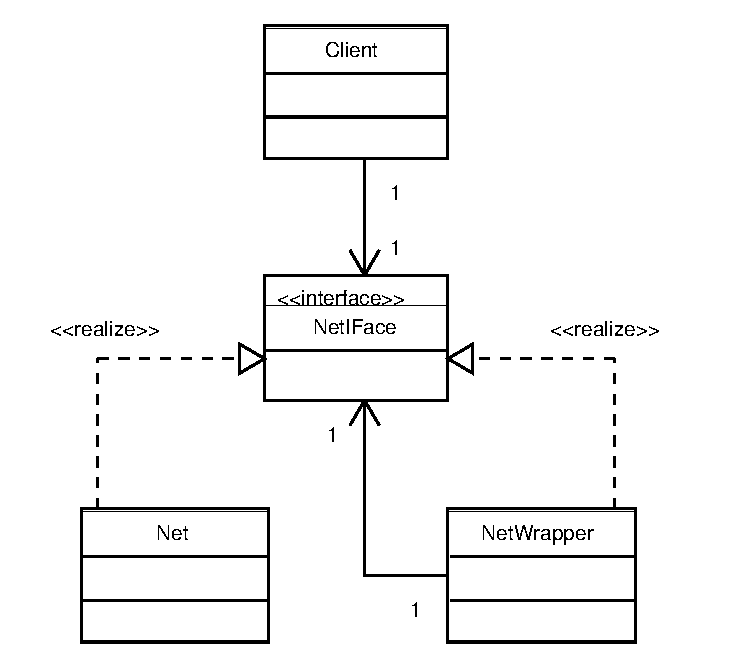
\includegraphics[scale=0.70]{img/composite.eps}
\caption{\figfont modello di composizione}\label{fig:comp}
\end{figure}

In questo modello, il client mantiene un riferimento all'interfaccia base per le reti neurali che, nella realt�, � implementata da due oggetti distinti: la classe rete neurale vera e propria ed una classe wrapper, o involucro, che viene istanziata passando come parametro un oggetto che implementi a sua volta l'interfaccia base e di cui ne occulta la struttura interna. Questa ultima operazione � ottenuta tramite una espansione del numero di nodi interni e una permutazione, nei limiti del possibile, delle posizioni degli elementi. Cos� facendo, si pu� consegnare al client un oggetto che rappresenta di fatto una rete neurale, come si aspetta, ma che potrebbe racchiudere la rete originale entro un numero potenzialmente senza limiti di incapsulamenti. Il client, di contro, non si accorger� di stare operando con una rete incapsulata o meno e di quanto profondo sia il livello di incapsulamento, bens� esso manegger� la rete in base al contratto specificato dall'interfaccia. Per una discussione pi� dettagliata di questo e molti altri pattern, � consigliata la lettura di \cite{designpattern}.\\
Da notare che, ovviamente, la metodologia di espansione adottata per occultare la struttura interna delle reti neurali non ne influenza affatto la conformazione, come descritto in sezione \ref{subsec:nnff}. Infatti, i nodi aggiuntivi non si collegano ai neuroni gi� presenti in alcun modo ma bens� concorrono a formare uno strato aggiuntivo interfogliandosi con essi per interallacciare i due livelli, cos� da espandere apparentemente la dimensione del singolo livello intermedio. Allo stesso modo, il processo di permutazione della posizione dei nodi non influenza l'ordinamento effettivo di visita dei nodi reali (importante in reti neurali feedforward, ad esempio), ma agisce solo su quei nodi che possono essere effettivamente scambiati di posizione; questo significa che, ad esempio, si potr� avere uno scambio di posizione fra nodi reali e nodi fittizi, cos� come anche fra neuroni reali appartenenti allo stesso livello che non presentano quindi collegamenti fra di loro ma solo verso altri nodi appartenenti ai livelli superiori e inferiori.

Il modello adottato permette di gestire le reti (nella figura della classe \texttt{NetManager}) e fornirle dietro richiesta occultandone il contenuto, proponendo ad ogni domanda per una stessa rete oggetti i cui componenti interni non variano ma la cui struttura � di volta in volta diversa. Infatti, sebbene i nodi di riempimento (anche detti nodi fittizi) vengano creati e inseriti all'atto dell'incapsulamento della rete neurale nel suo involucro e lasciati invariati nel tempo (cos� che un possibile attaccante non possa basarsi sull'analisi dei nodi che si ripresentano ad ogni richiesta o che invece variano nel tempo), la permutazione delle posizioni viene effettuata da parte del gestore a seguito di ogni richiesta per la specifica rete, ottenendo il risultato sopra descritto.

\subsection{Manager di reti}
Il gestore delle reti neurali, rappresentato dalla classe \texttt{NetManager}, � un complesso controllore per gli oggetti presenti nel sistema che ne regola l'accesso, il recupero delle informazioni associate alla singola rete neurale, l'impostazione dei parametri associati quali il fattore di quantizzazione o il fattore di espansione e permette il caricamento o l'eliminazione di nuovi elementi all'interno del sistema.

Il gestore delle reti neurali associa ad ogni singolo oggetto un valore intero per il recupero degli elementi su base 
identificatore. Esso presenta un tipo privato di oggetti interni non accessibili direttamente, pi� snelli e capaci di maneggiare la singola rete neurale, associati quindi singolarmente ad ogni nuovo elemento caricato nel sistema. Gli oggetti appartenenti a questa classe privata interna hanno alcune caratteristiche molto interessanti di seguito elencate:
\begin{itemize}
\item sono i reali responsabili del controllo sull'accesso alle reti neurali
\item contengono un semaforo binario per limitare le richieste soddisfatte a solo una per volta, accodando tutte le successive e servendole singolarmente in modo sequenziale
\item mantengono una rappresentazione della rete neurale affidata al loro controllo inserendola a priori in un involucro per occultarne il contenuto (si veda a tale proposito sezione \ref{subsec:cpc}), richiamando le funzioni di permutazione su di essa ogni volta che viene fornita verso l'esterno a seguito di una richiesta
\item ad essi � demandato il recupero delle informazioni sulla rete neurale in vari formati e livelli di completezza, cos� da implementare un efficace recupero di quest'ultime in base all'identit� del richiedente (ad esempio, a seconda che la richiesta provenga dal server per la manutenzione o dal client per l'uso).
\end{itemize}
Basandosi sull'ipotesi di corretto funzionamento degli elementi interni a cui � affidata la gestione della singola rete neurale, il gestore di sistema implementa funzioni per il recupero delle informazioni relative a tutti gli oggetti contenuti (e non solamente al singolo), per l'associazione di una singola rete neurale al suo identificatore, per il caricamento, l'eliminazione e addirittura l'aggiornamento di queste, per l'impostazione dei parametri su base identificatore con filtraggio preventivo e per la richiesta in merito alla possibilit� d'uso relativa alle reti neurali. Il compito del gestore delle reti neurali � sicuramente semplificato dall'uso degli elementi interni sopra descritti e questo comporta che esso sia limitato a funzioni di facciata molto semplici in termini di elaborazione.\\
La tecnica di delegazione delle mansioni fra i diversi elementi di un sistema � molto usata nella programmazione ad oggetti e permette, come in questo caso, di alleggerire e semplificare alcune classi a discapito dell'aggiunta di altri protagonisti che si fanno carico di far fronte a determinati compiti. In questo modo, pur aumentando il numero di classi presenti nel sistema (anche se spesso di poco, come in questo caso che prevede l'aggiunta di una sola classe ulteriore), risultano essere in generale pi� semplici e pertanto � pi� facile sia la comprensione da parte di terzi che la manutenzione o modifica.

\subsection{Modello unificato per reti neurali}
Il modello adottato per la rappresentazione delle reti neurali all'interno di NNSec merita una sezione a s� dedicata per vari motivi. Infatti, questo ha comportato addirittura delle modifiche agli algoritmi proposti nel protocollo originale che generalizzassero astraendo dal tipo di rete neurale maneggiata di volta in volta, proponendo un algoritmo unico adatto per ognuna di esse che non costringesse il flusso di esecuzione ad articolarsi su rami diversi a seconda dei dati.

\paragraph{Modelli diffusi.}
In letteratura, le reti neurali sono spesso rappresentate grazie all'uso di matrici e array. Infatti, supponendo di avere $ N $ nodi nella rete neurale logicamente numerati da $ 0 $ a $ N-1 $, il valore in essi contenuto pu� essere memorizzato tramite l'uso di un array di lunghezza $ N $ in cui ogni cella corrisponde al nodo avente indice pari a quello della cella stessa. Su questa base, si possono rappresentare i collegamenti fra i nodi (supponendo ad esempio che fra due nodi vi possa essere un solo collegamento) usando una matrice $ N\times N $, per cui il valore nella cella $ (i,j) $ rappresenta il peso del collegamento fra i nodi con indici rispettivamente pari a $ i $ e $ j $. La matrice � molto probabilmente sparsa e lo spreco di memoria consistente, ma l'accesso immediato ed efficiente. Una soluzione alternativa, meno performante ma pi� compatta in termini di memoria, � quella che prevede l'uso di liste collegate con indici, per cui ogni nodo mantiene memoria dei nodi ad esso collegati. In entrambi i casi, l'identit� del nodo � debole e rappresentata dal solo valore ad esso associato, una soluzione che non si presta per operare in NNSec. Inoltre, in entrambi i casi bisogna utilizzare una serie di inter-allacciamenti ulteriori fra i nodi per mantenere memoria della loro appartenenza ad un livello piuttosto che ad un altro, o una qualsiasi tecnica che raggiunga lo stesso scopo se necessario.

\paragraph{Classi dedicate.}
Per dare ad ogni nodo e anche ad ogni collegamento fra nodi un'identit� pi� forte sono state create due classi pubbliche interne all'interfaccia sviluppata per le reti neurali che proponessero appunto la possibilit� di maneggiare pi� facilmente nodi e collegamenti fra questi. La classe nodo d� la possibilit� ad esempio di associare al singolo elemento non solo un valore specifico, ma anche una propria funzione di attivazione e di uscita, una soglia, un gruppo (che rappresenta il livello di appartenenza) e ovviamente una serie di collegamenti da e verso altri nodi, cio� in entrata e in uscita dal nodo considerato. Allo stesso modo, la classe collegamento presenta la possibilit� di mantenere un valore e di fornire velocemente informazioni sul nodo di provenienza e di destinazione del collegamento considerato. Discostandosi quindi da un modello pi� geometrico basato su vettori e matrici, � stato utilizzato un approccio decisamente pi� orientato agli oggetti dove la singola rete neurale � costruita componendo i singoli elementi di base.\\
La possibilit� di impostare per un singolo neurone sia una funzione di attivazione che una funzione di uscita permette di comporre pi� funzioni in maniera facile e veloce, senza dover ricorrere a contorsionismi per elaborare un dato valore. Indicando la funzione di attivazione con $ f $ e la funzione di uscita con $ g $, si pu� immaginare la funzione di attivazione $ a $ associata al singolo nodo nella discussione teorica in sezione \ref{subsec:nn} come risultante dalla composizione delle precedenti, ovvero: $ a = g\circ f $.

\paragraph{Modello unificato.}
Utilizzando i mattoni descritti nel paragrafo precedente, � possibile adesso descrivere il modello unificato adottato in NNSec. Questo modello prevede la rappresentazione della rete neurale come array di nodi scandito in modo sequenziale. Ogni nodo � inserito all'interno del vettore nell'ordine di comparsa all'interno del sistema (cio�, in base alla posizione nel file di descrizione della rete neurale) e i collegamenti fra nodi sono memorizzati all'interno dei nodi stessi come collegamenti entranti o uscenti, quindi non vi � la necessit� di mantenerne ulteriore memoria separata. La scansione sequenziale prevede che durante l'analisi dei nodi (ad esempio in una sessione di uso della rete neurale) questi siano prelevati dal vettore in ordine e quindi elaborati. Per recuperare il valore di un nodo collegato ad un altro, � sufficiente partire da quest'ultimo, recuperare il riferimento relativo al collegamento in ingresso e a quest'ultimo domandare quale sia il nodo da cui scaturisce. Questa rappresentazione si presta in modo particolare per modelli feed-forward (fra cui � incluso anche il percettrone, inteso come degenerazione di tali modelli), infatti basta elencare i nodi nel file di descrizione della rete neurale nell'ordine in cui questi devono essere visitati e al resto penser� NNSec. Questo modello, pertanto, permette di astrarre dalla reale natura della rete neurale in uso e descrivere ognuna di queste con un modello unico adattabile a tutte le situazioni, la cui unica limitazione � il fatto che i nodi vengono visitati in ordine sequenziale (ma, del resto, il protocollo era concepito per percettroni e reti feed-forward, pertanto tutti i casi sono comunque accolti fra le braccia del nuovo modello).\\
L'unica questione che rimane in sospeso � come vengano espansi i livelli intermedi e come vengano permutati i nodi interni ad ogni livello, dato che il modello apparentemente non mantiene traccia dell'appartenenza di un singolo nodo ad uno specifico livello. La soluzione sar� discussa nel paragrafo seguente ma si osservi in questa sede il fatto che questo modello permette di astrarre dalla struttura multi-livello delle reti neurali e quindi mette a disposizione la possibilit� di descrivere potenzialmente reti neurali di qualsiasi tipo.

\paragraph{Occultamento.}
Il modello descritto introduce per ogni nodo un gruppo di appartenenza che pu� anche non essere impostato (ovvero avere valore nullo, o zero). Questo parametro pu� ovviamente essere utilizzato per legare fra loro un insieme di nodi che sar�, quindi, potenzialmente permutato in maniera del tutto casuale, come descritto in sezione \ref{subsec:nnff}. Infatti, il gruppo di appartenenza pu� essere visto come il livello a cui ogni nodo � associato e assegnare quindi a due nodi uno stesso gruppo significa collocarli in uno stesso livello della rete neurale. Inoltre, nella fase di inserimento dei nodi fittizi all'interno della rete neurale occultata questi vengono associati di volta in volta ad un gruppo specifico di livello intermedio il che comporta, come conseguenza, l'espansione in maniera del tutto casuale dei livelli intermedi. Questa, per altro, pu� essere controllata in modo molto fine attraverso un oculato assegnamento delle classi ai singoli nodi. In questo modo ci si ricollega alle osservazioni fatte in sezione \ref{subsec:nnff}, ovvero:
\begin{itemize}
\item il numero di livelli $ L $ pu� essere controllato nella fase di configurazione della rete neurale, in modo che questa operazione non influisca sul risultato finale ma renda l'illusione di una rete neurale contenente di fatto un livello intermedio aggiuntivo; infatti, se si desidera aggiungere un livello nascosto ulteriore basta dividere in due gruppi i neuroni appartenenti ad uno stesso livello e assegnare ai due gruppi classi di appartenenza diverse, con la sola limitazione che si pu� avere un numero massimo di livelli $ L_{max} $ pari al numero $ N $ di neuroni presenti all'interno della rete neurale, 
\item le dimensioni $ M_i $ in termini di numero di neuroni dei singoli livelli sono gestite a run-time da NNSec stesso, il quale introducendo neuroni fittizi nella rete neurale e distribuendoli in modo casuale fra i diversi livelli permette di avere valori $ M_i $ ogni volta diversi e assolutamente indipendenti da parametri relativi alla rete neurale in esame (come il numero di neuroni originali o il numero di livelli)
\end{itemize}
Con questa tecnica, i compiti di occultamento della rete e permutazione dei nodi sono lasciati in parte all'utente lato server (che ha la libert� di decisione sul numero di livelli, ovvero sulla lunghezza massima del cammino fra neuroni di ingresso e di uscita) e in parte al programma che si occupa di riempire in modo automatico i diversi livelli con nodi fittizi permutandone poi l'ordine e confondendoli con i neuroni originali. Tutto ci� pu� sembrare forse complicato a prima vista, ma consegna all'utente un modo raffinato, potente e flessibile per gestire la distribuzione dei nodi sui diversi livelli intermedi e conseguentemente il loro occultamento.\\
L'ipotesi su cui si basa questa idea � che i nodi appartenenti ad uno stesso livello non presentano collegamenti fra di loro, altrimenti l'ordine di visita assumerebbe importanza e non potrebbero essere permutati senza incappare in errori sul risultato. Inoltre, sarebbe consigliabile assegnare ad uno stesso livello solamente neuroni che presentano collegamenti in ingresso provenienti da nodi senza classe o con indice di classe inferiore e collegamenti in uscita verso nodi senza classe o con indice di classe superiore, proprio come in realt� vengono assegnati i neuroni ad un livello piuttosto che un altro in una rete feed-forward aciclica.

\paragraph{Ripercussioni sul protocollo.}
Tutto quanto sopra descritto si ripercuote infine sul protocollo originale. Infatti, come detto, viene usato in NNSec un modello di rete neurale che astrae dalla natura di percettrone o rete neurale con uno, dieci, cento livelli, ma bens� propone una generalizzazione unica per tutti questi tipi. Di conseguenza, � sorta la necessit� di trovare un algoritmo che a sua volta generalizzasse rispetto al tipo di rete e fosse applicabile al nuovo modello, senza dover ricorrere a due algoritmi diversi oppure un algoritmo unico che presentasse due rami di esecuzione diversi discriminando sulla tipologia di rete neurale a monte. Fortunatamente, i due algoritmi descritti dal protocollo originale per l'applicazione a percettroni e reti neurali multi-livello feed-forward (discussi in sezione \ref{sec:proto}) hanno molti punti in comune e differiscono solo nella fase di trattamento dei livelli intermedi, assente per il percettrone e piuttosto articolata per le altre reti neurali. Quindi, � bastato sviluppare un algoritmo che fosse una fusione dei due e che generalizzasse dal tipo di rete senza diramare il flusso di esecuzione a seconda dei dati proposti, ma bens� trattando il modello unico in un modo che fosse corretto per qualsiasi rete neurale in esso rappresentata. L'algoritmo risultante altro non � che l'algoritmo proposto per trattare reti neurali con un numero variabile di livelli intermedi, adeguatamente modificato per trattare il modello unico generico (ovvero anche i casi in cui il numero di livelli intermedi sia pari a zero). Questo, infatti, si adatta perfettamente anche al caso in cui tale modello descriva un percettrone, in quanto si basa alla fine sui nodi della rete neurale (e non sulla sua struttura) e su di questi fonda tutto il suo lavoro.

\paragraph{Pro e contro.}
Ovviamente, tutto questo ha sia dei pro che dei contro.\\
Prima di tutto, va detto che il modello permette di astrarre dal tipo di rete e di conseguenza conduce ad un numero minore di algoritmi coinvolti adatti a tutti gli usi e di gran lunga pi� semplici ed efficienti; infatti, dividere l'esecuzione su due algoritmi ed introdurre una guardia che discriminasse in base al tipo di rete avrebbe appesantito il tutto rendendo la gestione assai pi� complessa.\\
Di contro, per�, il modello unico � meno stringente e permette anche di descrivere reti neurali assolutamente senza senso e il cui risultato � del tutto imprevedibile, proprio perch� esso d� la possibilit� di disegnare qualsiasi tipo di rete neurale; del resto, per�, questo � anche il modo sbagliato di usare il software e davanti a queste situazioni si pu� fare poco perch� ogni programma, se usato malamente, dar� risultati inattesi. Quindi, si pu� dire che questo rovescio della medaglia non � cos� preoccupante, perch� rappresenta solo il caso in cui il software funziona male se usato male e questa �, del resto, la norma in molti casi.\\
Un cenno infine sulle responsabilit� degli utenti. Per quanto riguarda gli utenti lato client, l'uso di NNSec non comporta difficolt� e non richiede particolari conoscenze, sollevando da molte responsabilit� e occupandosi di tutti gli aspetti necessari all'espletamento del servizio. Di contro, lato server l'utente ha pi� libert� ma anche pi� responsabilit�: infatti, se da una parte il processo di occultamento della rete neurale pu� essere controllato in modo molto fine, dall'altro un errore in questo frangente potrebbe rendere del tutto vano lo sforzo. Anche in questo caso, non esistono compromessi e la libert� di decisione ha inevitabilmente un costo in termini di responsabilit�. In NNSec � stata scelta la via della flessibilit�, cercando di ottenere un potente mezzo con cui modellare le cose a proprio piacimento, a discapito della responsabilit� crescente in seno all'utente.

Da notare, infine, che il numero di livelli deciso in maniera implicita all'atto della stesura del file di descrizione della rete neurale rappresenta il valore $ L $ introdotto in sezione \ref{subsec:nnff}, mentre la successione data dai numeri di nodi associati ad ogni singolo livello � equivalente alla successione indicata con $ M_i $ sempre in sezione \ref{subsec:nnff}. Guardando questi parametri sotto questa luce si vede come l'implementazione finale non si discosti dal modello proposto in teoria e pertanto sono valide tutte le osservazioni fatte precedentemente basate appunto sui valori $ L $ e $ M_i $.

\section{Server}
Il subpackage \texttt{server} propone tutte le componenti utili alla fornitura dei servizi e alla configurazione dell'ambiente per una corretta interazione con i client, mettendo a disposizione anche una comoda GUI per permettere all'utente finale di interagire col sistema influenzandone il comportamento.

Sicuramente, tralasciando la GUI che altro non � se non un mezzo per semplificare la vita al gestore del sistema (descritta nelle sue componenti in appendice), il server propone alcune classi e spunti interessanti che lo rendono appetibile dal punto di vista del programmatore.\\ Infatti, senza scendere troppo in dettagli tecnici, esso basa il suo funzionamento sul noto pattern creazionale Factory e permette di servire pi� richieste contemporaneamente, aggirando di fatto la tecnologia a cui si appoggia. Inoltre, questo pacchetto racchiude la componente lato server a cui � richiesta la messa in pratica del protocollo e che rappresenta, quindi, una delle classi principali dell'intero progetto.\\
L'importanza di una interfaccia attraverso cui amministrare in maniera semplice e veloce l'intero sistema non � poi da trascurare e rappresenta una comodit� per chi si trova a dover fare fronte al problema, alleggerendo il lavoro e semplificando di non poco le gestione del server.

\subsection{Factory Remota}\label{subsec:remfac}
Una delle evoluzioni principali, nonch� uno degli aspetti pi� interessanti, del modello client/server � sicuramente la possibilit� di servire pi� client contemporaneamente senza dover accodare le richieste servendole singolarmente (una modalit� che si potrebbe definire rudimentale per l'offerta di servizi). Questa rappresenta sicuramente una caratteristica interessante anche e soprattutto in NNSec, dove il sistema lato server presenta e gestisce pi� reti neurali accedibili separatemente e indipendentemente l'una dall'altra.

Infatti, servendo un solo client per volta e rifiutando o (nel migliore dei casi) accodando le richieste successive, laddove due differenti domande siano per due differenti reti neurali si pecca sicuramente di inefficienza (per non parlare dell'efficacia della soluzione, la quale deficienza si ripercuote in termini di nervosismo per gli utenti che devono aspettare in coda quando la loro rete neurale � disponibile). Anche su macchine mono-processore, dove comunque le richieste verrebbero servite singolarmente, l'idea (che poi altro non � che la base dei sistemi multi-threading) di gestire pi� richieste contemporaneamente interallacciando la loro esecuzione permette di dare all'utente una risposta immediata in termini di accoglimento della domanda e l'impressione di avere un server a s� dedicato per la fornitura dei servizi. Anche perch�, bisogna osservare che effettivamente nelle fasi di trasmissione dei dati ed elaborazione lato client, il server risulta effettivamente disponibile per poter effettuare altre operazioni o dedicarsi ad altre richieste.\\
Si intuisce facilmente che una situazione in cui le richieste sono servite sequenzialmente (ad esempio, basandosi sull'ordine di arrivo) pu� anche portare ad un drastico allungamento dei tempi di attesa e questo � proprio il caso di NNSec. Infatti, se una rete neurale � composta da un numero particolarmente grande di nodi e collegamenti fra nodi, aumenta di conseguenza il traffico fra client e server per l'espletamento di una richiesta, il tutto appesantito dalla componente crittografica che rappresenta di fatto la parte pi� impegnativa in termini di tempo di calcolo. Ci� nonostante, il server non pu� in alcun momento interrompersi per dedicarsi ad un'altra richiesta e questo va a discapito dei tempi di risposta.\\
In quest'ottica, NNSec � stato progettato per poter rispondere a pi� client contemporaneamente, aggirando alcune limitazioni imposte dal linguaggio e la tecnologia scelta, come spiegato in sezione \ref{sec:commodel}.

\begin{figure}
\centering
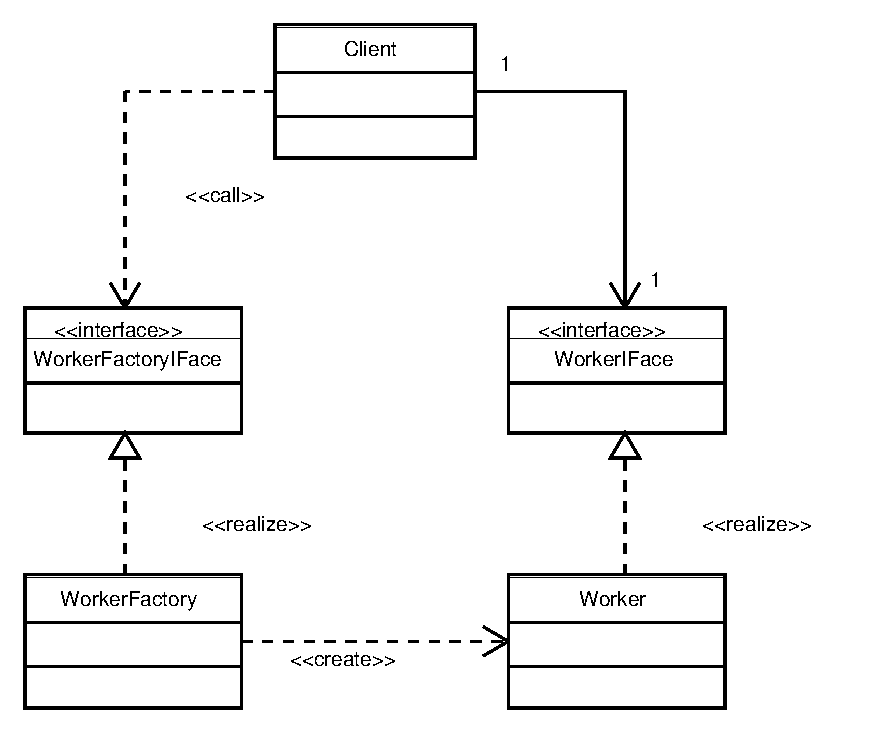
\includegraphics[scale=0.70]{img/factory.eps}
\caption{\figfont factory in NNSec}\label{fig:fact}
\end{figure}

In questo caso risulta utile l'applicazione di un pattern molto noto che assume il nome di Factory pattern ed � mostrato in figura \ref{fig:fact}, cos� come viene implementato ed utilizzato all'interno di NNSec. L'utilizzo di questo modello prevede una variazione alla struttura precedente, per cui il server altro non � che un oggetto in grado di istanziare a sua volta altre classi (potenzialmente, senza limiti, se non quelli imposti dalla macchina su cui esegue) a cui i client potranno fare riferimento per le loro richieste.\\
Questa organizzazione presenta alcuni risvolti positivi, di seguito elencati:
\begin{itemize}
\item il tempo di creazione di un riferimento da parte del server pu� essere considerato trascurabile, quindi ogni client avr� la possibilit� di interagire immediatamente col proprio oggetto associato vedendo accolte le proprie richieste entro breve termine
\item il singolo client che desidera avere solo informazioni sulla lista delle reti neurali disponibili non dovr� aspettare che la lunga e pesante elaborazione di altri client giunti prima di lui termini per poter avere ci� che desidera, ma sar� servito immediatamente
\item se il server presenta pi� reti neurali e si hanno richieste per reti neurali diverse da parte di diversi client, queste saranno servite contemporaneamente senza dover attendere (permutandone ogni volta le posizioni dei nodi come descritto nelle sezioni \ref{subsec:nnff} e \ref{subsec:cpc}); ovviamente se la richiesta � per una stessa rete neurale il modello adottato non risolve il problema ma in linea di massima permette di abbattere i tempi di attesa dei singoli client in molti casi
\end{itemize}
Sull'ultimo punto, � importante approfondire ulteriormente. Infatti, il problema dell'accodamento di richieste per una stessa rete neurale pu� effettivamente essere del tutto risolto con una tecnica che permetta di clonare l'oggetto in questione ad ogni richiesta di utilizzo. In questo modo, due client che richiedono una stessa rete neurale otterranno due copie identiche ma distinte di questa e potranno operare contemporaneamente. Ci� nonostante, esiste un rovescio della medaglia: la soluzione introduce un carico aggiuntivo a seguito di ogni richiesta che ritarda la fornitura del servizio a causa della necessit� di duplicazione delle reti neurali. Quest'ultimo aspetto potrebbe incidere sulle prestazioni nei casi in cui le reti siano di dimensioni molto elevate e si avrebbe un inevitabile peggioramento in tutti i casi in cui non vi siano richieste multiple. Infatti, nell'ipotesi che esista un solo client che richiede una determinata rete questo dovr� comunque sopportare il carico aggiuntivo dovuto alla duplicazione.\\
Non esiste un modo per determinare in maniera chiara e definitiva quale delle due soluzioni sia migliore o se esista una soluzione intermedia ottima, infatti:
\begin{itemize}
\item nel caso dell'accodamento si hanno migliori prestazioni su reti neurali accedute sporadicamente o che comunque ricevono poche richieste contemporanee, ma il comportamento degenera laddove si abbiano due o pi� richieste simultanee per una stessa rete neurale
\item nel caso della duplicazione sulle reti neurali si hanno migliori prestazioni in caso di pi� richieste contemporanee per una stessa rete neurale ma con un prezzo aggiuntivo dovuto alla copia della rete che pu� portare a peggioramenti significativi in caso di richieste singole
\item nel caso di soluzioni intermedie come quella che presuppone di dare la rete neurale al primo richiedente e produrre copie diverse per richieste successive, la quale sembrerebbe effettivamente un buon compromesso, sono introdotte tutta una serie di problematiche legate alla sicurezza dei dati in quanto le copie sarebbero fatte a partire da una rete neurale in uso e quindi contenente valori sensibili presenti all'interno dei singoli nodi
\end{itemize}

\subsection{I lavoratori}
Il lavoro, lato server, non � svolto dall'oggetto in ascolto per le richieste entranti, come accennato, ma bens� da un insieme di oggetti istanziati da quest'ultimo e associati al singolo client. Questi oggetti sono i lavoratori, rappresentati dalla classe \texttt{Worker}.

Questi elementi offrono tutta una serie di servizi nella loro interfaccia verso i client e si pongono come membrana fra di essi e il gestore delle reti, filtrando e regolando le richieste. Inoltre, presentano un ambiente interno impostabile dai diversi client, utile per la sessione di utilizzo delle reti neurali, che prevede la presenza di una chiave pubblica fornita dal client associato e alcuni valori concordati con quest'ultimo relativi all'utilizzo della rete neurale richiesta, variabili da interazione ad interazione (la chiave, invece, potrebbe restare anche la stessa, se i client decidono di non generarne di nuove a seguito di richieste successive).\\
Le istanze della classe \texttt{Worker}, ovvero i lavoratori, sono gli oggetti all'interno dell'intero progetto a cui � demandato il lavoro pi� impegnativo. Essi infatti possono espletare le richieste dei client nel caso questi richiedano informazioni sulle reti neurali disponibili, ma anche interagire con loro e calcolare l'output di una determinata rete neurale laddove pervenga una richiesta in tal senso. Se � vero che sar� preoccupazione dei client configurare ad-hoc l'ambiente dei lavoratori fornendo la propria chiave pubblica e concordando i parametri da usare durante l'elaborazione (e per questo, l'interfaccia di questi ultimi mette a disposizione tutti i metodi necessari), non si pu� dire altrettanto per quanto riguarda l'uso delle reti e il recupero dei valori di uscita: questa operazione, infatti, � affidata ai lavoratori che, pazientemente, dovranno computare i valori dei singoli nodi, passo dopo passo, interagendo (come gi� illustrato nell'analisi del protocollo) con i client al fine di ottenere il risultato atteso.\\
Questa fase rappresenta gran parte del carico computazionale dell'intero processo che, per come � strutturato il protocollo, � particolarmente sbilanciato e prevede lato server l'impegno pi� grosso per svolgere la componente pi� consistente dell'elaborazione.

\section{Client}
Il subpackage \texttt{client} introduce nel progetto le classi importanti per l'implementazione del protocollo dal punto di vista dell'utilizzatore finale, ovvero di chi vorr� servirsi delle reti neurali messe a disposizione come servizio remoto.

Questo pacchetto prevede prima di tutto una GUI minimale (descritta nelle sue componenti in appendice), ovvero una interfaccia grafica molto semplice tramite cui l'utilizzatore potr� decidere di creare o distruggere una connessione e reimpostare creandola ex-novo la propria chiave pubblica (e, di conseguenza, anche la chiave privata), decidendo tanto la lunghezza in numero di bit della chiave quanto un parametro di probabilit� relativo al fatto che la funzione di creazione operi correttamente. Gli aspetti riguardanti questi argomenti sono gi� stati discussi e approfonditi in sezione \ref{subsec:bigkey}.\\
Il pacchetto client per� non fornisce solamente le classi della GUI, bens� racchiude una serie di classi di gran lunga pi� importanti di questa, quali il modulo di comunicazione e il calcolatore, due elementi direttamente coinvolti nel protocollo proposto e aventi un ruolo abbastanza centrale.

\subsection{Modulo di comunicazione}
Il modulo di comunicazione rappresenta un'interfaccia fra il client e il server, o meglio fra il client e il lavoratore associato ad esso e residente sul server, un livello intermedio attraverso cui passano tutte le comunicazioni dell'utente finale e che si fa carico di effettuare le giuste chiamate di metodo per ottenere ci� che � richiesto.

Questo componente si preoccupa di stabilire una connessione in modo corretto con il server, passando per il registro apposito indicato dall'utente, richiedendo un lavoratore con cui poter interagire per le richieste future e di cui manterr� un riferimento nel tempo. Inoltre, ha la capacit� anche di troncare la connessione stessa dietro richiesta, il che molto semplicemente consiste nel cancellare il riferimento remoto al proprio lavoratore.\\
La funzione pi� importante del modulo di comunicazione, per�, � quella che lo vede interagire col proprio lavoratore associato per l'utilizzo di una rete neurale remota. Sebbene questa operazione possa sembrare abbastanza facile e nonostante il grosso del carico computazionale sia sulle spalle del server e non del client, questo componente svolge due ruoli importanti: da un lato si occupa della configurazione dell'ambiente del proprio lavoratore cos� che il risultato possa essere computato senza errori, mentre dall'altro istanzia ed esporta il calcolatore, un elemento a cui il lavoratore sul lato server si appogger� per svolgere delle funzioni che, altrimenti, sarebbe impossibilitato dal portare a termine.\\
Nell'impostare l'ambiente ed espletare le funzioni relative al protocollo discusso in sezione \ref{sec:proto}, il modulo di comunicazione svolge diversi compiti:
\begin{itemize}
\item si occupa di stabilire un valore relativo alle sessioni di cifratura e decifratura, ricavabile da alcuni parametri relativi alla rete che desidera usare e forniti dal lavoratore
\item concorda, o meglio convalida se possibile, il fattore di quantizzazione della rete neurale, utile per poter fornire valori in ingresso reali anzich� solo valori interi
\item istanzia un oggetto della classe \texttt{Calculator} in grado di applicare diverse funzioni ai valori in ingresso e lo fornisce al lavoratore, il quale lo user� per calcolare valori altrimenti non calcolabili
\item si fa carico della cifratura dei valori in ingresso, una volta stabiliti gli estremi per poter procedere, e la conseguente decifratura dei risultati ottenuti
\end{itemize}

\subsection{Il calcolatore}
Il calcolatore � nato come rimedio ad un problema che si � presentato durante le fasi di sviluppo e ha assunto immediatamente un ruolo importante all'interno del protocollo proposto: senza di lui, infatti, il server non sarebbe in grado di calcolare i risultati restituiti da alcuna rete neurale.

Questo componente � nato, come sar� spiegato in sezione \ref{subsec:fourfour}, dal problema del riferimento circolare. Di fatto, esso incapsula una serie di funzioni recuperabili tramite identificatore e necessariamente dislocate lato client in quanto non applicabili ai valori cifrati. Infatti, se grazie alle caratteristiche omomorfiche del cifrario molte funzioni lineari come la somma e la moltiplicazione possono essere effettuate in dominio cifrato ripercuotendosi sotto altra forma in dominio non cifrato, secondo necessit�, alcune altre come la sigmoide o la funzione segno o, pi� in generale, le operazioni non lineari non possono essere messe in pratica in alcun modo.\\
Questo limita la capacit� del server di operare in modo solitario e restituire quanto calcolato, ma lo costringe bens� ad interagire obbligatoriamente con il client che ha fatto richiesta per il risultato, nelle vesti appunto del calcolatore. Inoltre la fase di collaborazione, per come � stato progettato il protocollo, prevede due modalit� di interazione che purifichino i valori dalle impurit� assorbite durante la loro computazione lato server.\\
Il perch� dell'esistenza di due modalit� � presto spiegato. Come gi� illustrato parlando del protocollo, il risultato della computazione del valore di un determinato nodo passa tramite una specifica procedura che porta ad una doppia quantizzazione indesiderata ma inevitabile. Questo inconveniente viene quindi corretto al momento del calcolo del valore di attivazione del nodo, lato client, da parte del calcolatore, in quanto il valore viene decifrato ed � quindi facilmente gestibile anche in tal senso senza grossi sforzi. Risulta necessaria per� un'altra modalit� di funzionamento. Infatti, nel caso in cui un nodo presenti anche una funzione di uscita oltre alla funzione di attivazione (la prima � richiamata subito dopo l'altra, senza altre operazioni intermedie), questa riceve un valore che � gi� stato ripulito delle impurit� e non deve quindi in alcun modo essere dequantizzato un numero eccessivo di volte come nel caso precedente, pena il ritorno di risultati falsati.\\
Il calcolatore mette quindi a disposizione tutto il necessario per calcolare funzioni di attivazione e/o uscita e lascia al chiamante, ovviamente, la scelta della modalit� in cui si vuole eseguire.

\section{Modello di comunicazione}\label{sec:commodel}
NNSec prevede di sfruttare alcune delle caratteristiche pi� interessanti messe a disposizione dal linguaggio Java, tanto in termini di tecnologie (come RMI, o Remote Method Invocation) quanto in termini di librerie crittografiche (come il supporto a SSL, o Secure Socket Layer, descritto in \cite{ssl}). Ma non si limita qua. Appoggiandosi a queste primitive e combinandole con il modello di comunicazione presente in NNSec, in cui � adottata una struttura che vede coinvolti quattro elementi principali, si concorre ad ottenere caratteristiche di flessibilit�, accessi multipli concorrenti, sicurezza, efficacia ed efficenza.\\
Come questo sia possibile � spiegato nei punti che seguono:
\begin{itemize}
\item flessibilit�: l'uso della tecnologia RMI permette di sviluppare l'intero software come un'entit� unica e omogenea tralasciando quasi totalmente i dettagli relativi alla comunicazione via rete, racchiusi in una membrana fra client e server apparentemente invisibile che pensa a tutti i problemi relativi alla trasmissione/ricezione, gestione dei riferimenti remoti, invio dei dati e quant'altro
\item accessi multipli concorrenti: tramite metodologie di programmazione avanzate, integrate con quelle messe a disposizione dal linguaggio, si lascia spazio ad un modello ad accesso multiplo in cui un solo server � in grado di servire un numero potenzialmente senza limiti di client, gestendo il corretto accesso alle risorse del sistema ed evitando problemi quali la non integrit� sui dati
\item sicurezza: sfruttando, oltre al cifrario interno utile all'implementazione del protocollo proposto, canali cifrati stabiliti fra client e server, vengono innalzati i livelli di sicurezza e viene resa la vita un po' pi� dura ai possibili attaccanti; ovviamente, la sicurezza dell'intero sistema risiede sulla sicurezza delle componenti sottostanti e laddove questa verr� meno comporter� anche serie ripercussioni sull'intero progetto
\item efficacia ed efficenza: la risoluzione elegante di alcune problematiche di programmazione altrimenti piuttosto fastidiose ha permesso di sviluppare un software tanto efficace quanto efficiente, che raggiunga il risultato corretto senza disperdere le proprie energie; l'apparente complessit� si dissolve in soluzioni che prevedono una interazione chiara e pulita fra le parti, senza inutili complicazioni
\end{itemize}
Di seguito saranno analizzate pi� approfonditamente alcune aree tematiche interessanti relative ai punti di cui sopra, proponendo laddove siano introdotti problemi reali anche soluzioni reali.

\paragraph{Remote Method Invocation.}
NNSec pu� essere immaginato come un software monolitico eseguibile su di una macchina che permetta la multi-utenza, concepito per gestire richieste concorrenti da parte di pi� individui. Questa visione delle cose costringe comunque il progetto ad una frammentazione interna fra un componente centrale che rappresenta il cuore del programma, o core, e l'interfaccia utente intesa in termini di richieste verso il core. Partendo da questo punto di vista, lo sviluppo � progredito lungo questa strada ed � stata mantenuta questa visione del programma come entit� omogenea ma internamente separata in due parti.\\
A questo punto, entra in gioco la tecnologia RMI (ampiamente discussa e trattata in \cite{javarmi} tramite specifiche, guide ed esempi), o Remote Method Invocation, una evoluzione logica delle pi� datate RPC (Remote Procedure Call), nata con l'avvento dei linguaggi ad oggetti e ad essi associata. Infatti, una volta concepito il software come sopra esposto, tramite l'uso di questa tecnologia frapposta nelle comunicazioni fra core e interfaccia utente si possono dislocare i diversi oggetti componenti il programma su una rete (ma anche sulla stessa macchina, mantenendo la struttura originale) permettendo comunque loro di comunicare come se residenti tutti su una stessa unit� fisica. Questo concetto cerca di avvicinare il modello client-server puro, non decisamente proprio di NNSec, verso un modello ibrido che mantiene ancora una parentela col precedente ma che lascia immaginare il prodotto finale come un'entit� unica e indissolubile (le cui parti sono assolutamente inutili l'una senza l'altra).

\paragraph{Secure Socket Layer.}
Per quanto riguarda la sicurezza, una regola sempre valida � che questa non � mai abbastanza. Inoltre, le specifiche del protocollo descritto nel capitolo \ref{cap:one} impongono che la comunicazione fra client e server avvenga su un canale cifrato. NNSec crea quindi fra le parti coinvolte (client e server) un canale a sua volta cifrato basandosi sull'ormai affermato protocollo SSL nato appunto con lo scopo di fornire comunicazioni sicure sulla rete e descritto in \cite{ssl}.\\
Questa scelta, seppure innegabilmente importante, introduce non poca complessit� nel progetto e qualche pensiero di troppo per l'utilizzatore finale. Infatti, tanto chi gestir� il server quanto chi vorr� usufruire dei servizi tramite il client, sar� costretto a produrre o convalidare un certificato allo scopo di poter stabilire correttamente la comunicazione. Va detto che, del resto, Java offre tutti gli strumenti (compresi alcuni utili programmi) per ottenere in modo semplice e veloce quanto serve, quindi il tutto non rappresenta niente di particolarmente preoccupante.

\subsection{I quattro moschettieri}\label{subsec:fourfour}
La parte pi� rilevante dell'intero progetto non � ovviamente la GUI che permette all'utente finale di interagire con client e/o server, n� tantomeno il parser che permette di caricare in modo automatico e veloce una nuova rete a caldo, tutti elementi importanti del programma ma non direttamente coinvolti nell'implementazione del protocollo. Ci� che attira l'attenzione e che effettivamente rappresenta il cuore di NNSec � il modello di comunicazione vero e proprio fra client e server, messo in pratica da sole quattro classi (di cui, per altro, una ha solo un ruolo marginale). Queste classi implementano di fatto il protocollo descritto in capitolo \ref{cap:one}.\\
La tecnica di comunicazione adottata permette di risolvere in modo pulito alcuni problemi di progetto abbastanza rilevanti e aggirare con eleganza tutta una serie di limitazioni di cui soffre il normale modello di comunicazione client-server spesso proposto in applicazioni basate su RMI. Di seguito, sono discussi alcuni aspetti importanti del modello di comunicazione e verr� proposta di volta in volta una veloce scappatoia (spesso disarmante  nella sua semplicit�) per sfuggire da apparenti vicoli cechi, terminando con l'illustrazione del modello di comunicazione nella sua totalit�.

\paragraph{Riferimento circolare.}
Il modello di comunicazione che nasce spontaneo da una prima analisi del protocollo � abbastanza semplice. Basti pensare che se � vero che la parte client chiama la corrispettiva componente server per usufruire dei suoi servizi, quest'ultima a sua volta ha bisogno di potersi appoggiare al chiamante per i motivi illustrati in sezione \ref{subsec:req} (e che, per brevit�, non saranno discussi nuovamente in questa sede). Questo modello per� introduce in modo abbastanza subdolo una dipendenza circolare fra le due parti coinvolte per cui l'una non ha senso di essere senza l'altra durante una sessione collaborativa.\\
Ci� potrebbe anche essere trascurato (sebbene una dipendenza circolare del genere sia come una bomba ad orologeria pronta ad esplodere) se non fosse che l'uso di RMI rende impossibile la compilazione di due classi cos� fatte. Infatti, per poter usufruire dei vantaggi offerti da RMI, posto che un oggetto di una classe \texttt{A} voglia sfruttare i servizi di un oggetto di una classe remota \texttt{B}, il primo dovr� poter contare su una interfaccia di riferimento detta \texttt{B\_Stub} che presenta gli stessi metodi remoti offerti da \texttt{B} e si occupa della comunicazione sulla rete (oltre a tutta una serie di cose meno importanti da questo punto di vista). Va detto che l'interfaccia \texttt{B\_Stub} � creata a partire dalla classe gi� compilata \texttt{B}.\\
Nel caso specifico di NNSec, per�, la faccenda si fa pi� complessa: infatti, se \texttt{A} ha bisogno di \texttt{B\_Stub}, cos� anche \texttt{B} ha bisogno di \texttt{A\_Stub} e sia \texttt{A} che \texttt{B} nel loro codice fanno riferimento alle rispettive altrui interfacce. Pertanto, la classe \texttt{A} non pu� essere compilata in quanto non riesce a trovare \texttt{B\_Stub} fra le classi disponibili e pertanto non pu� essere creata \texttt{A\_Stub} e la stessa cosa vale anche per \texttt{B}.\\
Nessuna delle due classi pu� essere compilata, quindi, il che vuol dire che l'intero programma non pu� funzionare. Ovviamente, questa non � una eventualit� gradita in alcuna situazione.

\begin{figure}
\centering
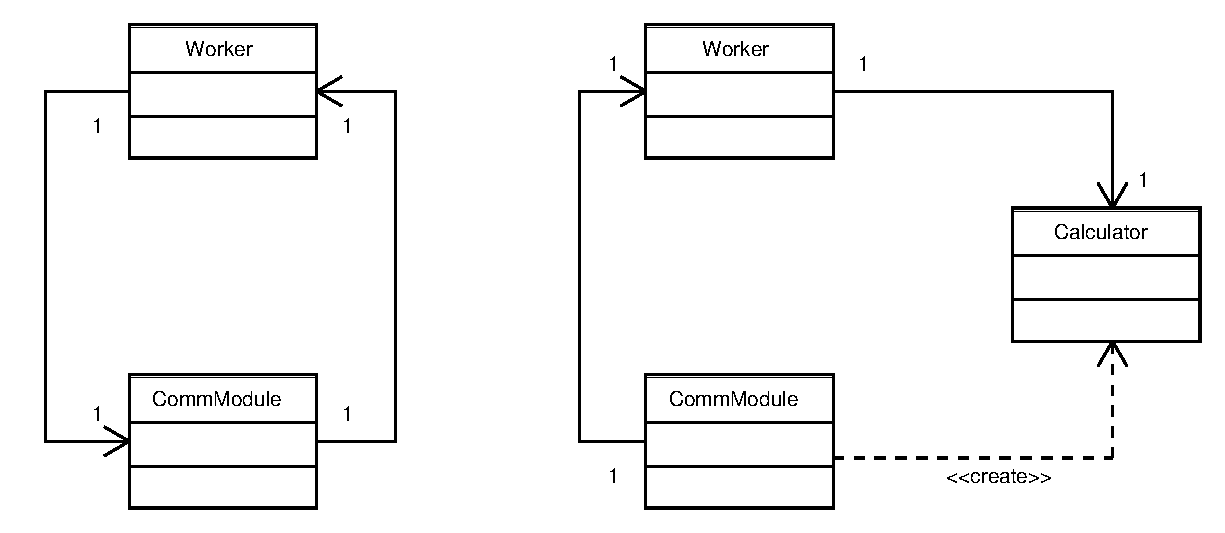
\includegraphics[scale=0.60]{img/circdep.eps}
\caption{\figfont modello di dipendenza circolare, senza e con classe funzione}\label{fig:cdep}
\end{figure}

La soluzione adottata in NNSec � per la verit� tanto semplice ed efficace quanto spesso invisibile agli occhi di molti che perdono fin troppo tempo tentando di risolvere un problema del genere.\\
Fermandosi a riflettere, ci si accorge subito che se il server � una entit� monolitica indivisibile, questo non � altrettanto vero per la componente client che pu� in realt� essere divisa in pi� parti indipendenti e egualmente funzionali. Infatti, per risolvere la questione, basta disaccoppiare il client vero e proprio dai servizi che esso offre e inglobare questi ultimi in una terza classe (che, di fatto, rappresenta una classe funzione e nient'altro) il cui riferimento sar� passato direttamente alla parte server all'atto della chiamata. Cos� facendo, si passa da un modello a due attori ad un modello che prevede tre attori ed elimina completamente qualsiasi dipendenza circolare (con il piacevole effetto di poter compilare e, quindi, eseguire il programma finale).\\
Il modello delle relazioni fra client e server (rappresentati rispettivamente dalle classi \texttt{CommModule} e \texttt{Worker}) prima e dopo l'aggiunta della classe funzione (nella forma della classe \texttt{Calculator}) � riportato in figura \ref{fig:cdep}.

\paragraph{Factory remota.}
Uno dei problemi principali nell'uso di RMI � rappresentato dal fatto che avendo un solo oggetto remoto (il server) in grado di offrire servizi, se questo � gi� impegnato nel tentativo di soddisfare una richiesta, tutte le richieste successive saranno rifiutate o, nella migliore delle ipotesi, accodate in attesa di poter essere prese in considerazione.

Questo problema � gi� stato discusso in sezione \ref{subsec:remfac}, ma viene qua richiamato perch� rappresenta uno dei nodi cruciali per cui il modello di comunicazione prevede quattro elementi e non meno. � importante, infatti, richiamare i concetti esposti parlando del pattern Factory che, come descritto, separa il ruolo di chi svolge effettivamente i compiti demandati al server da quello di chi invece istanzia oggetti in grado di servire le richieste stesse. In questo modo, i client possono fare domanda per un oggetto ad essi associato che serva ai loro scopi, e tale richiesta sar� soddisfatta molto velocemente. A loro volta, interagendo con il riferimento assegnatoli lato server, potranno operare sugli elementi messi a disposizione dal server stesso avendo l'illusione di essere i soli ad operare nell'ambiente. In realt�, questo non accade di norma, dato che la possibilit� che pi� client stiano accedendo nello stesso momento al server non � poi cos� remota in uno scenario reale, ma permette di soddisfare, quando possibile, pi� richieste in parallelo, abbattendo di fatto i tempi di attesa dei singoli client.

Va detto che, parlando di RMI, si aggiunge una componente ulteriore al modello, rappresentata dal registro. Infatti, una volta istanziato l'oggetto Factory, questo va posto su un registro di nomi che associ la sua posizione sulla rete (nella forma di un riferimento idoneo) ad un identificatore univoco. La richiesta dei client dovr� quindi passare attraverso il registro, il quale fornir� loro il riferimento di cui sopra (o stub) a cui essi potranno rivolgere le loro domande. Questo altro non � che un oggetto che presenta la stessa interfaccia lato server ma che incapsula al suo interno tutta una serie di dati per contattare l'elemento desiderato e un insieme di metodologie mirate all'espletamento dei servizi sulla rete.
\begin{figure}
\centering
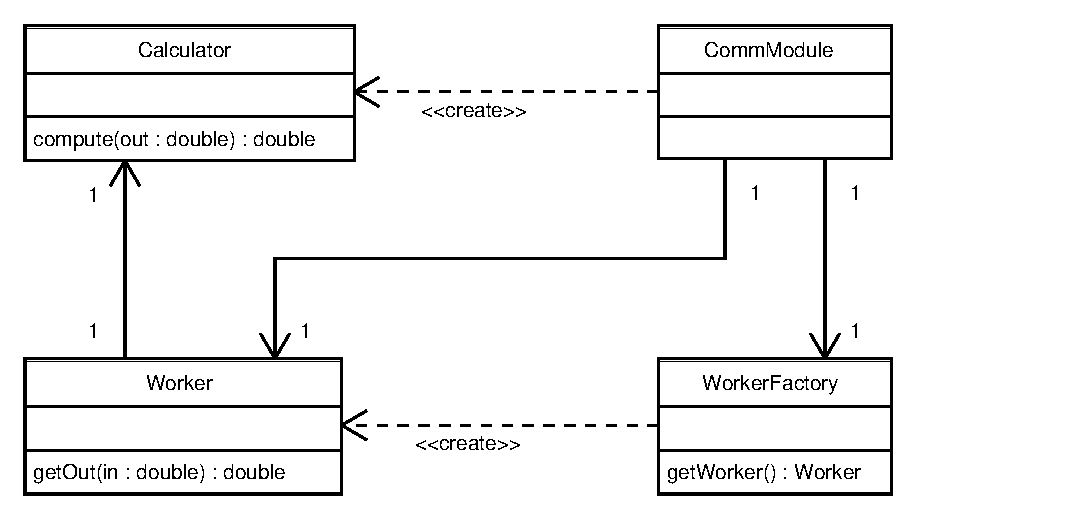
\includegraphics[scale=0.70]{img/fourfour.eps}
\caption{\figfont i quattro moschettieri}\label{fig:four}
\end{figure}
\paragraph{}
Arrivati a questo punto, sono stati gi� introdotti tutti gli attori coinvolti nel modello di comunicazione adottato da NNSec. Dal problema del riferimento circolare si intuisce che tre degli attori saranno le componenti di comunicazione lato server e lato client e la classe funzione istanziata e passata dal client al server durante la chiamata (rispettivamente, le classi \texttt{Worker}, \texttt{CommModule} e \texttt{Calculator} di NNSec). In aggiunta a queste, dall'intuizione riguardante l'introduzione di una factory remota per poter soddisfare contemporaneamente pi� richieste, � presente un quarto elemento che crea di fatto le componenti di comunicazione lato server (le classi \texttt{Worker} di NNSec) per poter gestire in modo concorrente pi� richieste da parte dei client (questa � la classe \texttt{WorkerFactory} di NNSec). Il modello appena descritto � esplicitato in forma grafica in figura \ref{fig:four}.
\paragraph{}
Basandosi sugli elementi di cui sopra, la comunicazione si articola in pochi semplici passi, di seguito esposti:
\begin{itemize}
\item Il client contatta il server (o meglio, una factory remota che rappresenta la componente server); in realt�, la chiamata rispetta lo standard imposto da RMI, per cui il client contatta un registro apposito su una determinata macchina in ascolto su una specifica porta a cui potr� fare richiesta per localizzare il server che sar�, infine, contattato direttamente.
\item La componente factory istanzia un oggetto dedicato (esportandolo per renderlo visibile da oggetti remoti) a cui il client potr� fare riferimento per le sue richieste successive, e lo restituisce a quest'ultimo. Per tutta la durata della connessione, il client potr� colloquiare con il riferimento ottenuto senza dover effettuare successive richieste per ottenere ulteriori riferimenti o servizi.
\item Per poter usufruire di una rete neurale, il client far� richiesta tramite il suo oggetto dedicato che risiede sul server per riuscire a bloccare la rete neurale desiderata, recuperarne i dati sensibili e intraprendere l'elaborazione passando (dopo averlo esportato per abilitarne la visibilit� remota) un riferimento remoto ad un oggetto funzione a cui il server, rappresentato dall'oggetto dedicato relativo al client, potr� fare riferimento richiedendo particolari servizi a seconda delle necessit� durante l'espletamento delle sue funzioni; al termine dell'esecuzione, l'oggetto client otterr� i valori di uscita della rete neurale.
\end{itemize}
\begin{figure}
\centering
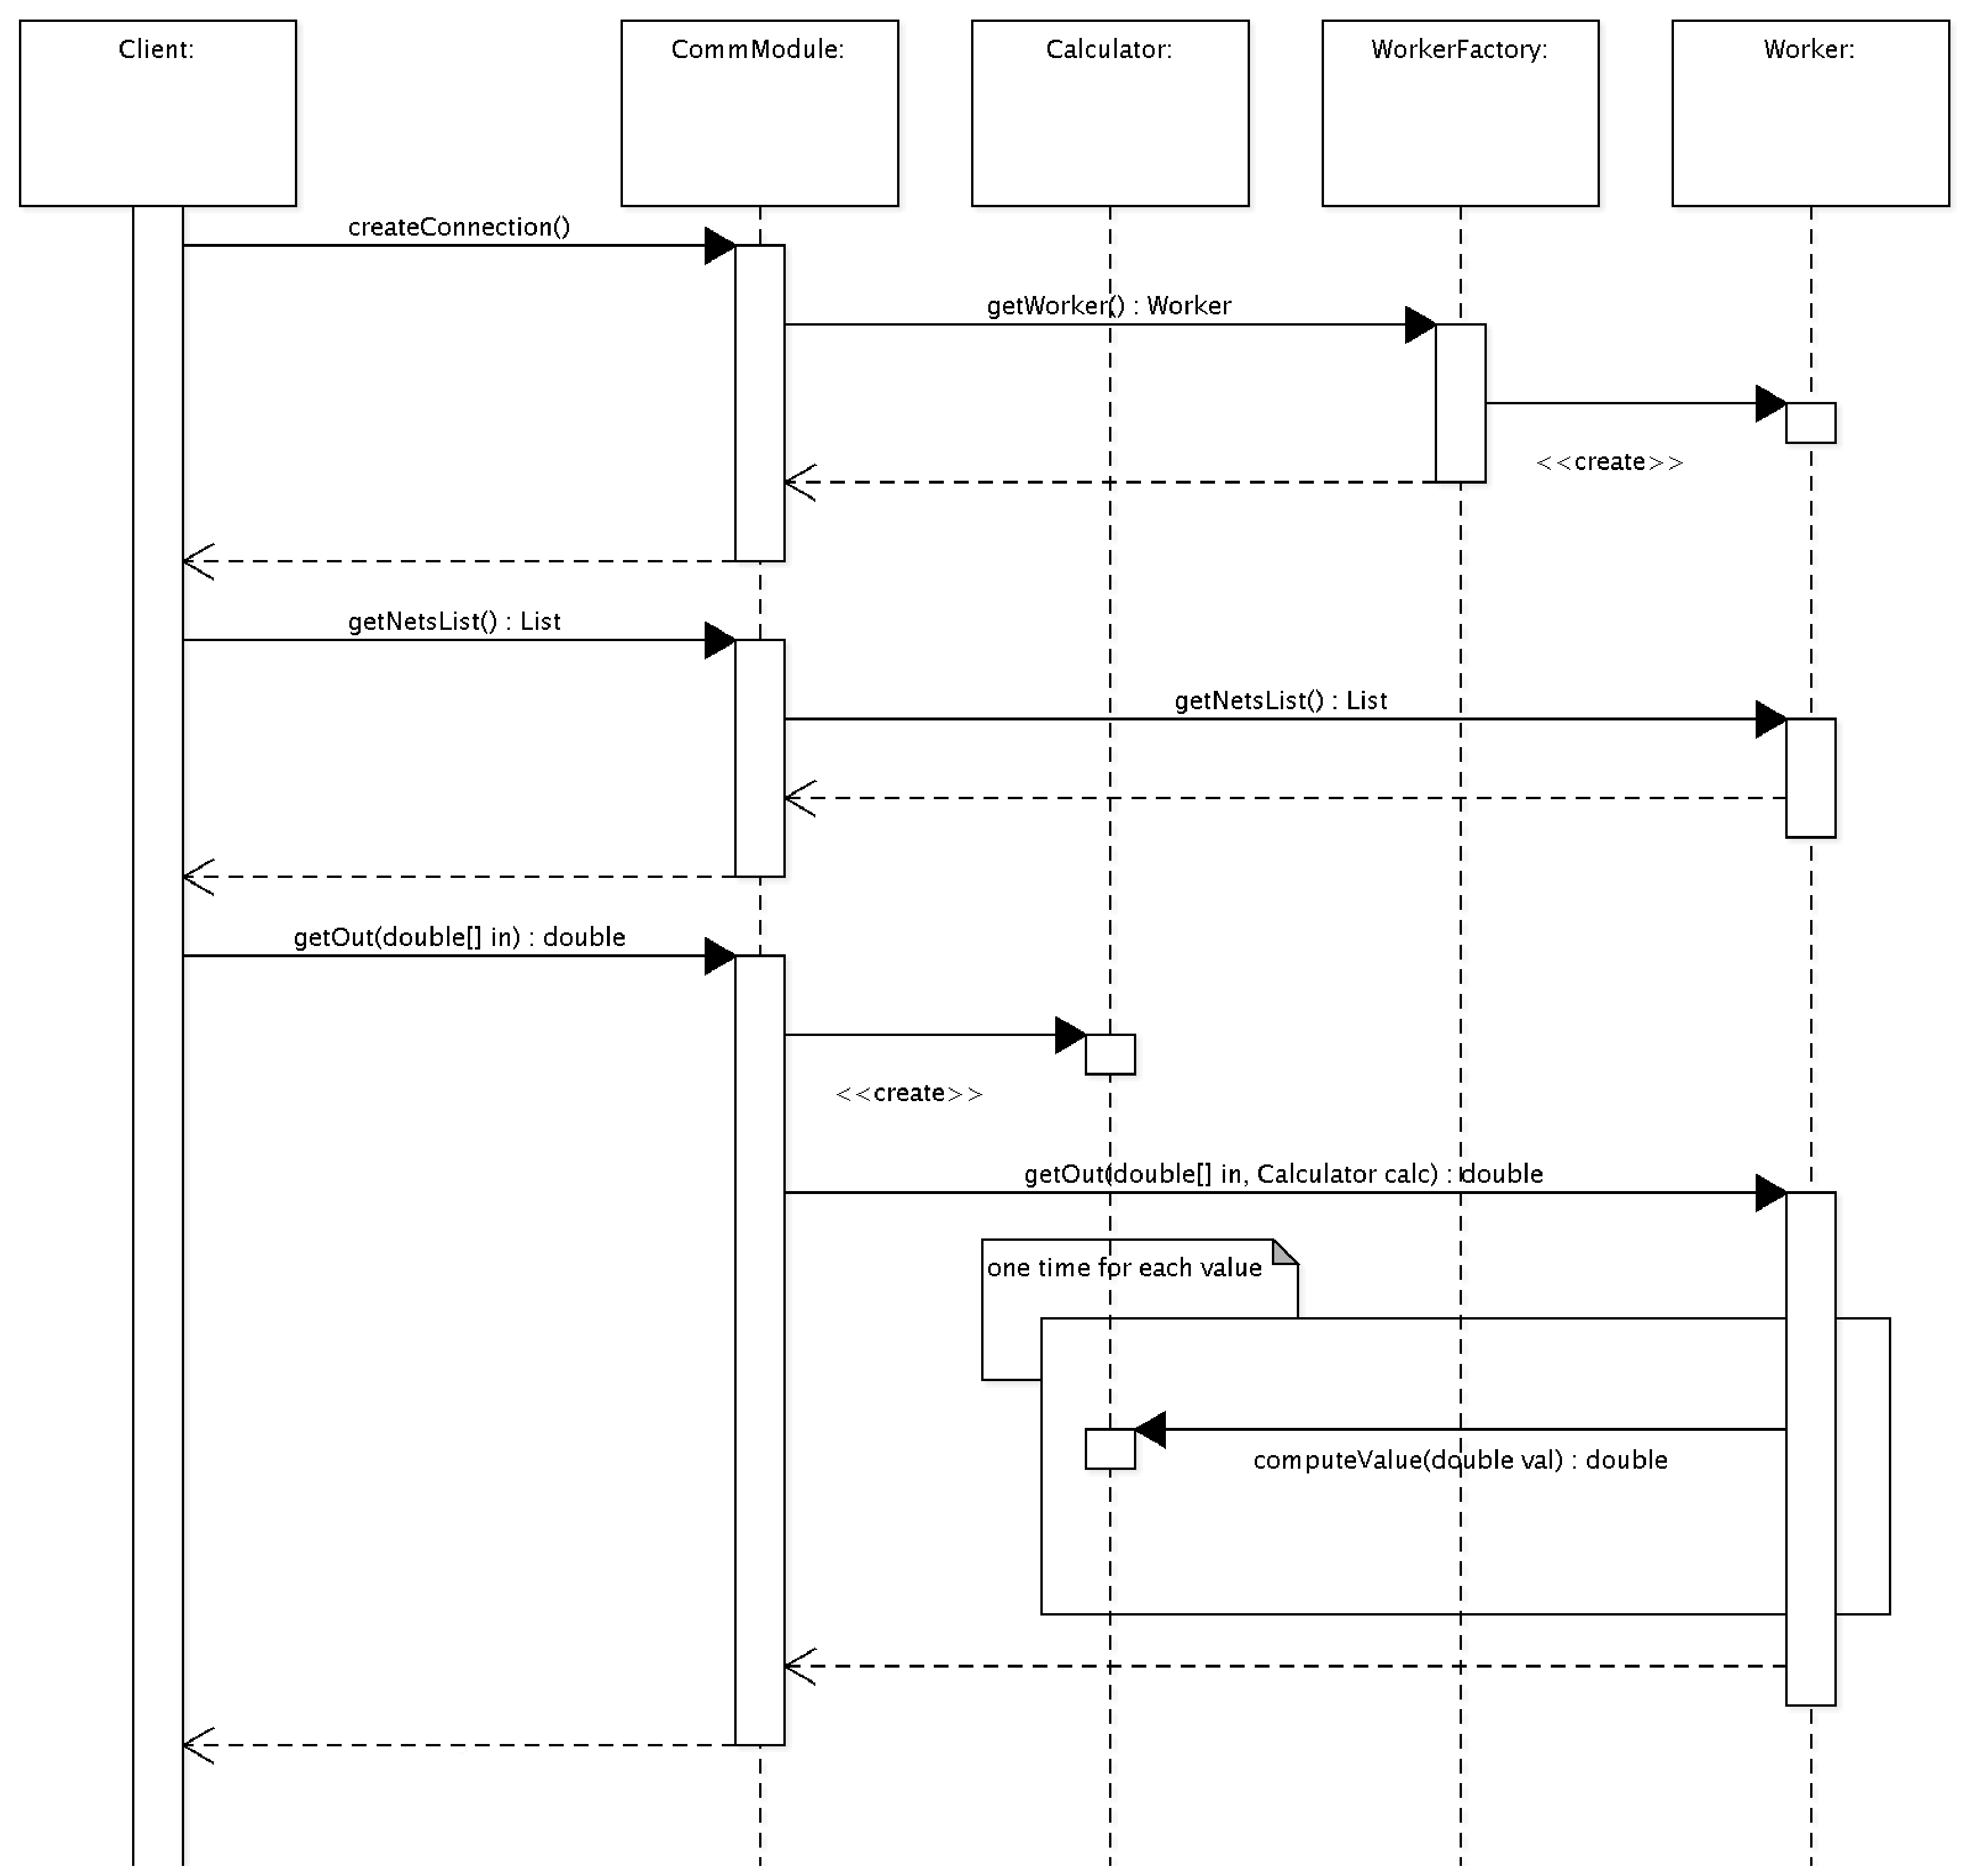
\includegraphics[scale=0.20]{img/seqdiag.eps}
\caption{\figfont diagramma di sequenza del modello di comunicazione (semplificato)}\label{fig:seqdiag}
\end{figure}
Un esempio in forma di diagramma di sequenza, semplificato rispetto all'originale, � riportato in figura \ref{fig:seqdiag}

\paragraph{}
Le quattro classi discusse, chiamate nell'ambito del progetto NNSec ``i quattro moschettieri'', rappresentano perci� il cuore del progetto, di fatto l'insieme di classi che implementano il protocollo cos� come descritto nel capitolo \ref{cap:one} e discusso in \cite{proto}, semplicemente appoggiandosi ad elementi di ambiente (come il gestore delle reti neurali o il parser) necessari per servizi e richieste che esulano dal protocollo stesso ma che risultano necessari.\\
Il modello di interazione fra questi elementi � il risultato di uno studio approfondito e propone in pochi elementi svariate tecniche e tecnologie, prese in prestito tanto dalla teoria quanto dagli strumenti messi a disposizione dello sviluppatore al giorno d'oggi. Il tutto ben amalgamato per raggiungere i risultati ottenuti: l'implementazione del protocollo proposto, ovvero la componente principale nonch� il cuore di NNSec.

\chapter{Prove Sperimentali}\label{cap:three}
\epigraph{Non testare mai una condizione d'errore che non sai come gestire.}{Linea di Guida di Steinbach per la Programmazione}

NNSec � stato ovviamente testato sotto determinate condizioni e modalit�, tanto per verificarne il corretto funzionamento quanto per valutarne il comportamento in relazione alla variazione di alcuni parametri (quali il numero di nodi fittizi, il fattore di quantizzazione utilizzato per gestire valori reali, etc.). Ci� che risulta � un quadro completo che fornisce un'idea di come NNSec si comporter� in un potenziale ambiente reale.

Per poter usare NNSec in ambiente distribuito (ma alcuni di questi accorgimenti sono validi anche per l'uso in locale) sono necessari dei passaggi obbligatori che concorrono ad ottenere un corretto funzionamento. Sar� quindi discussa tutta la fase preparatoria sia lato server che lato client per poter utilizzare NNSec. Questo comporta la preparazione, distribuzione e uso di certificati e la stesura di un file di policy che regoli le potenzialit� del server.\\
Infine, saranno analizzati alcuni parametri chiave che andranno ad influire sulle prestazioni di NNSec, come gi� accennato, proponendo risultati e tempistiche, ma anche cercando di stabilire una sorta di regola che permetta di predire un futuro quantomeno plausibile a partire da determinate impostazioni. Questo � molto importante anche nell'ottica di voler comprendere quale sia effettivamente un tetto massimo approssimativo per le possibilit� d'uso di NNSec.\\
Quello che segue � in parte preso direttamente dalla documentazione sulla sicurezza in Java, in particolare dalle sezioni relative a JSSE. Per approfondimenti e/o chiarimenti, fare riferimento alla documentazione ufficiale in lingua originale a partire da \cite{javasec}.

\newpage

\section{Configurare il server}
Per chi intende proporre un server NNSec (quindi, per chi intende mettere a disposizione le proprie reti neurali) ci sono alcuni passi forse tediosi ma necessari da percorrere, prima di poter raggiungere lo scopo. Questo lo si pu� mettere in conto come il prezzo da pagare per avere un p� di sicurezza in pi� (che non guasta mai).

\subsection{Certificati}
Quello di cui il gestore di server NNSec necessita per poter stabilire una connessione con i client che si appoggi ad un tunnel SSL � creare un cos� detto \textit{keystore} e riempirlo con appropriati elementi. In termini piuttosto semplici, si pu� pensare ad un \textit{keystore} come un portachiavi in cui sono immagazzinate tutte le chiavi locali utilizzabili dal server, o meglio tutte le coppie di chiavi pubblica/privata la cui parte pubblica � poi esportata per essere utilizzata dai client. Un elemento del \textit{keystore} � anche detto \textit{keyEntry} e tramite questo si pu� realizzare un certificato da fornire ai client cos� che questi possano gestirlo e inserirlo nel proprio \textit{truststore} (trattato in sezione \ref{subsec:ccer}).\\
La procedura per creare un \textit{keystore}, preparare una \textit{keyEntry}, inserirla nel \textit{keystore} e ricavarne un certificato valido � abbastanza semplice e si articola in pochi passi, di seguito elencati. Per fare quanto descritto � richiesto il programma \texttt{keytool}, solitamente distribuito insieme al Java Development Kit.
\lstset{basicstyle=\footnotesize}
\begin{itemize}
\item Per prima cosa � necessario creare un \textit{keystore} ed aggungervi una coppia di chiavi pubblica/privata. � possibile farlo in un unico comando, riportato di seguito. L'esempio mostra alcune linee spezzate su pi� righe grazie all'introduzione di una barra. Questo non avviene in casi reali ma � dovuto ad esigenze di spazio.
\begin{lstlisting}
 % keytool -genkey -alias nnsec -keyalg RSA \
     -keystore keystore 

 Enter keystore password:  nnsecks
 What is your first and last name?
 [Unknown]:  Michele Caini
 What is the name of your organizational unit?
 [Unknown]:  lci
 What is the name of your organization?
 [Unknown]:  unifi
 What is the name of your City or Locality?
 [Unknown]:  Florence
 What is the name of your State or Province?
 [Unknown]:  FI
 What is the two-letter country code for this unit?
 [Unknown]:  IT
 Is CN=Michele Caini, OU=lci, O=unifi, L=Florence, \
   ST=FI, C=IT correct?
 [no]:  yes

 Enter key password for <nnsec>
 (RETURN if same as keystore password):  <CR>
\end{lstlisting}
Vengono poste come si pu� notare alcune domande di carattere generale a cui rispondere, come alcuni dati relativi all'utente. Questo crea il \textit{keystore} che il server user�. � possibile aggiungere una validit� temporale a questo oggetto passando il parametro  \textit{validity} seguito da un numero rappresentante un intervallo in giorni.\\
Intuitivamente, il parametro \textit{genkey} indica la necessit� di generazione di una coppia di chiavi il cui identificativo � indicato dal parametro \textit{alias}; in modo simile, si capisce che il parametro \textit{keyalg} indica l'algoritmo da utilizzare nella fase di generazione delle chiavi mentre il parametro \textit{keystore} definisce il nome dell'archivio (in altri termini, il nome del file contenente il \textit{keystore} vero e proprio)
\item Adesso, � necessario esportare un certificato auto-convalidato. Ovviamente, se il client non si fida di chi mantiene il server, questa procedura non � molto adatta in realt�, piuttosto si dovr� ricorrere ad una \textit{Certification Authority} che supervisioni sulla generazione e convalidi i certificati coinvolti. Nel caso di esempio, quanto necessario lo si pu� ottenere in modo semplice e immediata.
\begin{lstlisting}
 % keytool -export -alias nnsec -keystore keystore \
     -rfc -file nnsec.cer

 Enter keystore password:  nnsecks
 Certificate stored in file <nnsec.cer>
\end{lstlisting}
Il certificato cos� ottenuto � pronto per essere distribuito ai client che ne faranno richiesta tramite un mezzo di comunicazione qualsiasi, affinch� la connessione su canale SSL possa essere stabilita facilmente.\\
Per quanto riguarda i parametri, \textit{export} indica la richiesta di esportazione della chiave relativa all'identificatore fornito come argomento con \textit{alias}, mentre come nel caso precedente \textit{keystore} indica il file contenente l'archivio e \textit{file} il nome del file in cui archiviare il certificato. In merito al parametro \textit{rfc}, laddove presente questo comporta la creazione di un certificato in un formato di codifica stampabile, ovvero delimitato all'inizio e alla fine dagli identificatori:
\begin{lstlisting}
  -----BEGIN CERTIFICATE-----
     Corpo del messaggio
  -----END CERTIFICATE-----
\end{lstlisting}
\end{itemize}

\subsection{File policy}
Il file di \textit{policy} per il linguaggio Java stabilisce le politiche adottate nei confronti di svariate risorse. I file di \textit{policy} e la loro sintassi sono discussi a partire da \cite{javasec}. Fra le cose interessanti, ad esempio, si possono definire intervalli di indirizzi IP per cui le connessioni in ingresso siano accettate o meno o ancora stabilire quali porzioni di un filesystem sono accessibili, da chi e con quali privilegi. Ovviamente, laddove questo si scontra con il sistema operativo sottostante, in alcuno modo ci� che definisce il file di \textit{policy} va contro ci� che � stabilito dall'ambiente ospite e in tali casi sono apportate tutte le limitazioni imposte dal sistema operativo con priorit� rispetto alle altre.\\
Di seguito � riportato il file di \textit{policy} di esempio fornito insieme al server NNSec.
\begin{lstlisting}
  grant {
    permission java.net.SocketPermission "*", \
      "accept,connect,resolve";
    permission java.security.SocketPermission "*", \
      "accept,connect,resolve";
  };

  grant {
    permission java.util.PropertyPermission "user.home", "read";
    permission java.io.FilePermission "${user.home}${/}", "read";
    permission java.io.FilePermission "${user.home}${/}*", "read";
  };
\end{lstlisting}
Questa configurazione � fin troppo permissiva e non si presta ad essere usata in situazioni reali, ma rappresenta un ottimo compromesso per la fase di test in quanto non pone quasi alcuna limitazione sulle connessioni in ingresso e sulle possibilit� di accesso al filesystem.\\
La sintassi e le modalit� di stesura di un file di \textit{policy} esulano dallo scopo di questa tesi e per ogni approfondimento � consigliato fare riferimento alla documentazione ufficiale, a partire da \cite{javasec}.

\subsection{Lanciare il server}
Una breve ma importante nota va fatta sulle modalit� di esecuzione del server. Questo � invocato da riga di comando, passando tutto ci� di cui � stato discusso fin'ora come parametri. In particolare, la riga di comando risultante � la seguente (supposto di usare l'archivio originale chiamato \texttt{nnsecserver.jar}):
\begin{lstlisting}
 % java -Djava.security.policy=policy \
     -Djavax.net.ssl.keyStore=keystore \la stampa
     -Djavax.net.ssl.keyStorePassword=nnsecks \
     -jar nnsecserver.jar
\end{lstlisting}


\section{Eseguire il client}
Per chi vuole utilizzare il client NNSec (quindi, per chi intende sfruttare le reti neurali remote messe a disposizione), invece, la cosa � leggermente meno complicata ma non priva di accorgimenti. Anche in questo caso, si pu� mettere il tutto in conto come il prezzo da pagare per avere un p� di sicurezza in pi� (che non guasta mai).

\subsection{Certificati}\label{subsec:ccer}
Una volta venuto in possesso di un certificato valido, fornito dal possessore del server NNSec in un modo qualsiasi, chi vuole utilizzare il client deve creare un \textit{truststore}, ovvero in parole povere un archivio in cui saranno contenuti tutti i certificati ritenuti validi da poter utilizzare per i propri scopi. Le voci presenti nel \textit{truststore} sono anche dette \textit{trustedCertEntry}.\\
� possibile importare i nuovi elementi all'interno del \textit{truststore} come segue (rifacendosi all'esempio visto nelle sezioni precedenti):
\begin{lstlisting}
 % keytool -import -alias nnseccert -file nnsec.cer \
     -keystore truststore

 Enter keystore password:  trustword
 Owner: CN=Michele Caini, OU=lci, O=unifi, L=Florence, \
   ST=FI, C=IT
 Issuer: CN=Michele Caini, OU=lci, O=unifi, L=Florence, \
   ST=FI, C=IT
 Serial number: 46e29d22
 Valid from: Sat Sep 08 15:01:22 CEST 2007 until: \
   Fri Dec 07 14:01:22 CEST 2007
 Certificate fingerprints:
   MD5: 76:8B:9E:4A:E3:5A:00:AE:65:8E:B5:DF:47:FE:E7:06
   SHA1: \
     9C:0F:C8:DC:C8:5E:CC:CD:25:94:E4:A4:F3:70:14:85:7C:9C:A3:8E
 Trust this certificate? [no]:  yes
 Certificate was added to keystore
\end{lstlisting}
La procedura, evidentemente, � molto semplice. Anche in questo caso sono poste poche, semplici domande in merito agli identificativi forniti insieme al certificato, stampati per poter essere esaminati. Il compito dell'utente client � finito, non resta che lanciare NNSec e sfruttare le reti neurali remote secondo le proprie necessit�.\\
Intuitivamente, per quanto riguarda i parametri passati da riga di comando, � possibile dire che \textit{import} indica la necessit� di importare una determinata voce all'interno dell'archivio identificandola col nome passato come argomento di \textit{alias}, \textit{file} indica il nome del file che contiene il certificato relativo mentre \textit{keystore} rappresenta il nome del file dell'archivio, ovvero del \textit{truststore} vero e proprio.

\subsection{Lanciare il client}
Come gi� sottolineato, bisogna soffermarci anche in questo caso sulla modalit� di esecuzione del programma. Questo � invocato da riga di comando, come anche il server, tramite l'uso di appositi parametri (supposto di usare l'archivio originale chiamato \texttt{nnsecclient.jar}):
\begin{lstlisting}
 % java -Djavax.net.ssl.trustStore=truststore \
     -Djavax.net.ssl.trustStorePassword=nnsects
     -jar nnsecclient.jar
\end{lstlisting}

\section{Parametri}
L'uso di righe di comando piuttosto lunghe per mandare in esecuzione sia client che server pu� apparire scomodo, in realt�.\\
Sebbene non percorsa in questo caso, Java mette a disposizione almeno una seconda strada che consiste nel caricare nell'ambiente i valori relativi alle variabili indicate direttamente da file. Questa via comprende la preparazione, una volta per tutte, di un file contenente coppie chiave/valore da cui il programma attinger� all'avvio. Del resto, questo modello vincola all'uso di determinati file o costringe l'utente, una volta avviato il programma, alla ricerca nel filesystem di un file e conseguente caricamento ad ogni esecuzione. Un altro metodo possibile � l'inclusione di un pannello attraverso cui, a run-time, impostare le diverse variabili d'ambiente, secondo necessit�.\\
La via scelta in NNSec � quella sopra discussa, ovvero il passaggio dei parametri tramite riga di comando. In ogni caso, futuri sviluppi potrebbero integrare comode interfacce tramite cui impostare i parametri direttamente da programma o attraverso cui caricare file contenenti tali valori.

\section{NNSec, RMI e router}
Per quanto riguarda l'uso di NNSec sulla rete Internet, laddove la macchina su cui eseguono client e/o server si trovi dietro ad un router, devono essere fatte alcune precisazioni. Infatti, con le configurazioni di cui sopra il programma (client e server) funziona senza particolari problemi in locale ma si lamenta quando viene tentato l'uso distribuito, ovvero nei casi in cui client e server siano dislocati su macchine diverse.
\paragraph{Indirizzi.}
Nel caso, per altro molto probabile, in cui si vogliano usare client e server su macchine diverse poste potenzialmente ai due angoli opposti della terra, possono presentarsi problemi nella risoluzione degli indirizzi in pi� punti del processo di interazione fra client e server, come ad esempio al momento della chiamata verso il registro di nomi o quando si cerca di stabilire una connessione fra modulo di comunicazione e factory remota e via dicendo. I problemi citati possono essere di vario genere e dovuti alle pi� svariate cause; per fare un piccolo esempio (ma potrebbero essere molti di pi�), su sistemi GNU/Linux una riga solitamente innocua nel file \textit{/etc/hosts} pu� rivelarsi una spina nel fianco cercando di usare RMI. Queste situazioni, apparentemente semplici da affrontare e risolvere, in realt� sono abbastanza subdole perch� il programma termina con una eccezione che indica il rifiuto di stabilire una connessione da parte del server e non d� indicazioni sulla reale motivazione. La ricerca del perch� pu� quindi risultare lunga ed estenuante, anche alla luce del fatto che su questo aspetto la documentazione � un po' scarsa e incompleta.\\
Per capire il problema � meglio procedere con un esempio. Si immagini la fase in cui la componente server crea una \texttt{WorkerFactory} e la esporta legando lo \textit{stub} di quest'oggetto ad un determinato identificatore su un registro di nomi, cos� che i client possano recuperarlo ed usarlo (per quanto riguarda gli \textit{stub}, sono stati introdotti motivandone l'esistenza in sezione \ref{subsec:fourfour}). In termini molto semplici, si pu� pensare alla fase di creazione ed esportazione dello \textit{stub} come un'operazione in cui questo viene istruito sul come svolgere specifiche funzioni e gli viene fornito un indirizzo a cui fare riferimento per le chiamate di metodi remote. Questo indirizzo � recuperato lato server facendo richiesta al proprio sistema e se la macchina si trova in una rete locale l'indirizzo che verr� incapsulato nello \textit{stub} non sar� valido per il rintracciamento sulla rete Internet. Peggio ancora, sotto determinate condizioni allo \textit{stub} potrebbe essere fornito l'indirizzo 127.0.0.1 che rappresenta la macchina locale; una volta che questo riferimento � poi consegnato ai client esso far� richiesta sulla rete verso la stessa macchina su cui opera dove, ovviamente, non risiede il server, generando un'eccezione.\\
La soluzione esiste e consiste nell'aggiunta di una ulteriore opzione fra i parametri d'invocazione per client e server, ovvero una stringa:
\begin{lstlisting}
-Djava.rmi.server.hostname=<ip>
\end{lstlisting}
In questo caso, ad \textit{<ip>} va sostituito l'indirizzo che il router della sottorete presenta sull'interfaccia di rete affacciata verso l'esterno, ovvero sulla rete Internet. Ovviamente, il valore di \textit{<ip>} pu� differire (molto probabilmente lo far�) fra client e server.\\
Questo parametro permette di indicare al programma il nome dell'host (in questo caso, l'indirizzo ip) che deve essere associato agli stub remoti per gli oggetti creati localmente e a cui queste interfacce fanno riferimento, cos� da permettere ai client l'invocazione di metodi sugli oggetti remoti stessi senza che essi sollevino eccezioni del tipo \textit{connessione rifiutata}. Il valore predefinito per questa propriet� � l'indirizzo IP della macchina su cui il programma esegue ma, se questa opera dietro un firewall, potrebbe non essere una informazione utile. Infatti, non sempre la Java Virtual Machine � in grado di ottenere automaticamente il nome del dominio in cui si trova o, come nel caso proposto, l'indirizzo IP corretto da utilizzare.
\paragraph{Porte.}
Un altro problema, non di minore importanza, � dato dal fatto che l'ipotetico router sopra citato che separa la rete locale dalla rete Internet potrebbe operare da firewall o potrebbe comunque essere presente un firewall nella rete locale che limita le connessioni da e verso gli utenti. Questo � uno scoglio facilmente superabile ma bisogna fare molta attenzione.\\
Dal punto di vista del server NNSec, questo deve poter riceve collegamenti in ingresso sulla porta 1099 (in modalit� predefinita, ma tale numero pu� essere liberamente cambiato), ovvero la porta su cui ascolta il registro di nomi. Purtroppo per� questo non basta. Infatti, gli oggetti esportati dal server quali la factory remota o i lavoratori associati ai diversi client possono essere posti in ascolto su una qualsiasi porta maggiore di 1023 e non prevedibile a priori. Quindi, devono essere permesse tutte le connessioni su queste porte senza alcuna esclusione. Questo potrebbe rappresentare una limitazione alla sicurezza della rete locale, ma si osservi che un comportamento simile � adottato anche dai server Web e non rappresenta potenzialmente un problema.\\
Dal punto di vista del client NNSec, invece, vale un discorso simile al precedente. Infatti, questo per poter comunicare ed interagire col server dovr� poter esportare un oggetto calcolatore per la computazione dei valori di attivazione/uscita di un nodo. Questi oggetti, ancora, possono risultare in ascolto su una qualsiasi porta con indice maggiore di 1023 e bisogna quindi permettere connessioni in ingresso su tali porte. Come nel caso precedente, la problematica risulta nella configurazione di un eventuale firewall cos� da ridurre i rischi di questa operazione. Allo stesso pari del punto precedente, si osservi che questo � lo stesso comportamento adottato ad esempio da software P2P e non introduce quindi alcuna novit� o stravolgimento.

\section{Risultati}
Ultimi, ma non ultimi, alcuni risultati sperimentali sull'uso di NNSec. Una volta terminato lo sviluppo di NNSec � stato necessario portare avanti alcuni test variando i parametri di funzionamento del software per valutarne il comportamento sotto diversi punti di vista e carico variabile.

Bisogna prima di tutto soffermare un attimo la discussione sul cosa sia veramente interessante o meno da studiare e valutare. Questo perch� per quanto riguarda NNSec non ha molto senso valutare la complessit� algoritmica nelle fasi di interazione fra client e server, ovvero durante l'espletamento vero e proprio del protocollo. Infatti, si capisce facilmente che il grosso del carico � dovuto alla presenza di algoritmi a chiave pubblica/privata e quest'ultimi hanno una complessit� di gran lunga superiore a quella quasi lineare delle fasi di interazione, per cui rappresentano la componente principale sotto questo aspetto. Per una analisi dettagliata di questi algoritmi ed uno studio completo sulla loro complessit�, fare riferimento a \cite{paillier} e \cite{brics}.\\
Un aspetto che vale la pena di studiare, invece, � quello del carico in termini di pacchetti e conseguentemente in byte sulla rete, per vedere come questo varia al variare dei parametri fondamentali come il numero di nodi fittizi o il fattore di quantizzazione utilizzato per rappresentare i numeri reali in interi positivi e via dicendo. Questo pu� essere molto interessante perch� essendo NNSec un software basato sul modello client-server pu� incidere notevolmente sul carico di rete e quindi sulle prestazioni di quest'ultima. Allo stesso modo, sono interessanti le osservazioni sui tempi di esecuzione, sia per quanto riguarda il tempo totale che il tempo in seno al client e al server (dai quale si pu� dedurre, infine, il tempo di trasmissione).
\paragraph{Teoria.}
Intuitivamente, � possibile aspettarsi che il comportamento sia linearmente dipendente dal numero di nodi della rete neurale.\\
Infatti, eccezion fatta per le fasi di interazione che prevedono il recupero di un riferimento lato server da parte del client e il recupero della lista delle reti neurali disponibili (operazioni a carico fisso e indipendente dai parametri delle diverse reti), si pu� immaginare che per ogni nodo appartenente a livelli intermedi o di uscita di una specifica rete neurale vi sia una fase di comunicazione fra client e server, ovvero la fase in cui essi interagiscono per la computazione del risultato. Questo � vero, poich� per ogni nodo fra quelli sopra indicati il server dovr� ricorrere ai servizi del client cos� da poterne estrapolare il valore associato.\\
\begin{figure}
\centering
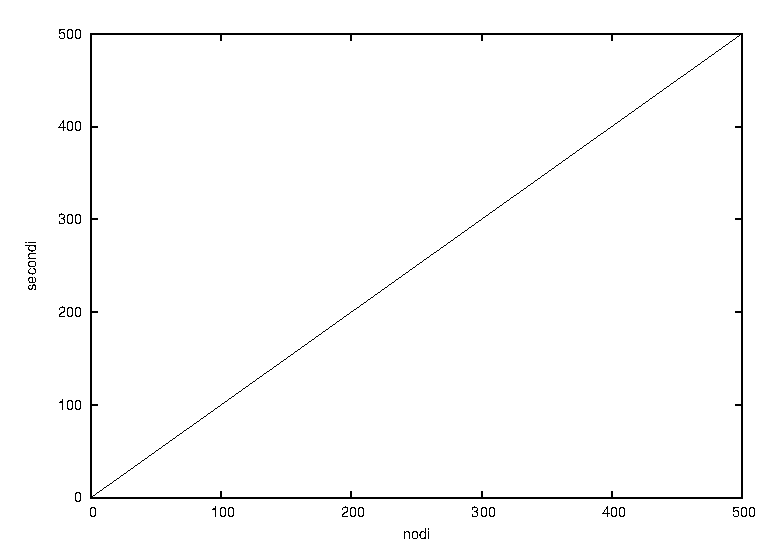
\includegraphics[scale=0.75]{img/idea.eps}
\caption{\figfont comportamento atteso}\label{fig:yx}
\end{figure}
Teoricamente, quindi, il comportamento atteso � qualcosa di simile a quello riportato in figura \ref{fig:yx}, ovvero una funzione del tipo $ y = f(x) = x $. Questo � vero tanto per quanto rigurda il tempo di esecuzione totale che per il numero di pacchetti (e conseguentemente il flusso di dati sulla rete), mentre poco si pu� dire sui tempi lato client e lato server senza un'analisi pi� attenta e approfondita.\\
Anche se si potrebbe studiare in modo pi� completo il comportamento atteso in linea teorica, � pi� conveniente discutere direttamente i dati sperimentali ed estrapolare il comportamento adottato a partire da una situazione reale in cui il software sviluppato viene mandato in esecuzione.
\paragraph{Pratica.}
Per quanto riguarda le prove fatte, l'ambiente di test utilizzato � descritto nei punti che seguono:
\begin{itemize}
\item Le macchine su cui server e client sono stati mandati in esecuzione sono descritte di seguito, rispettivamente:
\begin{itemize}
\item Pc Desktop con processore Intel Core 2 Quad (2.40GHz) e 4Gb RAM, sistema operativo GNU/Linux Debian e java versione 1.5 (Java 5).
\item Laptop con processore Intel Core Duo (2GHz) e 1024Mb RAM, sistema operativo GNU/Linux Gentoo e java versione 1.5 (Java 5).
\end{itemize}
I due dispositivi sono stati messi in comunicazione attraverso una rete LAN a cui entrambe le macchine erano direttamente connesse.
\item La rete neurale utilizzata per i test presenta 60 nodi di ingresso, 12 nodi intermedi e 1 nodo di uscita. Questa rete � stata addestrata con dati presi dall'UCI Machine Learning Repository\footnote{http://mlearn.ics.uci.edu/MLRepository.html} e relativi alla distinzione di segnali lanciati contro cilindri metallici o pietre sotto varie angolazioni e condizioni. La rete neurale � stata sottoposta, in realt�, ad overfitting, ovvero si � lasciato che imparasse a memoria gli esempi visti: infatti, lo scopo non era creare una rete neurale in grado di generalizzare, ma piuttosto capace di dare il risultato esatto sugli esempi sottomessi per poter valutare il comportamento di NNSec e la sua correttezza a prescindere da quella della rete neurale. L'idea di una rete neurale che sbagliasse facendo sospettare un errore in NNSec non era, effettivamente, cosa gradita e viste le necessit� questa operazione � giustificata.
\item La dimensione delle chiavi pubbliche/private � stata scelta pari a 1024 bit, ovvero sono stati generati grazie ai metodi messi a disposizione dalla classe \texttt{BigInteger} valori primi interi esprimibili con 1024 bit. In \cite{reccomendation} � trattata la questione della gestione delle chiavi e si possono trovare cenni sulla lunghezza consigliata per le chiavi in numero di bit a seconda dell'algoritmo usato e del tempo di vita previsto (dove per tempo di vita si intende l'intervallo di tempo necessario affinch� la chiave possa essere potenzialmente rivelata); da notare che l'uso di chiavi con lunghezza pari a 512 bit � sconsigliato se non in fasi di test o per effettuare prove arbitrarie, mentre l'uso di chiavi di lunghezza pari a 1024 bit pu� assumere un ruolo rilevante anche in ambienti reali.
\item Il fattore di quantizzazione � stato scelto pari a 9, ovvero tale per cui il fattore effettivo risultante fosse equivalente a $ 10^9 $. Questa scelta pu� sembrare azzardata e potrebbe essere avanzata l'ipotesi di ridurre tale fattore a 6, cos� da diminuire la complessit� di calcolo. Bisogna per� osservare che i valori ottenuti a seguito della quantizzazione e rappresentazione nel dominio degli interi positivi saranno poi espressi, una volta cifrati, con un minimo di 1024 bit (ovvero la lunghezza minima utilizzabile per le chiavi pubbliche/private). Quindi, il tentativo di limitare le loro dimensioni nella fase di quantizzazione � reso vano dalle operazioni di cifratura; ne segue che si pu� liberamente scegliere un fattore come quello sopra riportato (ovvero, pari a 9) in modo che ci� non influisca sulle operazioni a seguito di eventuali troncamenti dei valori decimali, basandosi sul fatto che esso non influir� in modo eccessivamente consistente in maniera negativa neanche sulla complessit� dei calcoli presenti all'interno del protocollo.
\end{itemize}
Prima di cominciare, va notato che si pu� limitare l'analisi sul traffico alla sola fase di interazione per l'uso della rete. Infatti, il carico dovuto alla connessione fra client e server e al recupero della lista delle reti neurali disponibili � fisso nel primo caso (in cui discende dall'interazione fra client e registro dei nomi e alla chiamata verso la factory remota per recuperare un riferimento ad un lavoratore associato) e lineare in base al numero di reti neurali presenti nel secondo caso. Ovviamente, entrambi questi valori non sono in alcun modo relazionati al numero di nodi fittizi o al fattore di quantizzazione usato per gestire i numeri reali e, pertanto, risultano di scarso interesse.

\begin{table}[ht]
\begin{center}
\begin{tabular}{|c||c|c|c|c|c|}
\hline
& \multicolumn{5}{|c|}{\textbf{Fattore di Quantizzazione = 9}} \\
\cline{2-6}
\textbf{Nodi}& \textbf{tempo (s)} & \textbf{client (s)} & \textbf{server (s)} & \textbf{pacchetti} & \textbf{byte} \\
\hline
\hline
12 + 1 & 27 & 7 & 20 & 204 & 71608 \\
12 + 2 & 27 & 7 & 20 & 223 & 74157 \\
12 + 3 & 28 & 8 & 20 & 217 & 75089 \\
12 + 4 & 29 & 8 & 20 & 228 & 77121 \\
12 + 5 & 29 & 9 & 20 & 242 & 79814 \\
12 + 6 & 30 & 9 & 20 & 242 & 80677 \\
12 + 7 & 30 & 10 & 20 & 263 & 83835 \\
12 + 8 & 31 & 10 & 20 & 254 & 84032 \\
12 + 9 & 31 & 11 & 20 & 281 & 87634 \\
12 + 10 & 32 & 11 & 21 & 285 & 89477 \\
12 + 15 & 35 & 13 & 21 & 326 & 99095 \\
12 + 20 & 38 & 16 & 22 & 365 & 107634 \\
12 + 25 & 40 & 18 & 21 & 375 & 114412 \\
12 + 30 & 43 & 20 & 22 & 437 & 125771 \\
12 + 40 & 49 & 26 & 23 & 512 & 143591 \\
12 + 50 & 55 & 31 & 24 & 592 & 162007 \\
12 + 75 & 69 & 43 & 26 & 792 & 208763 \\
12 + 100 & 81 & 54 & 27 & 958 & 251834 \\
12 + 125 & 97 & 67 & 30 & 1167 & 299168 \\
12 + 150 & 112 & 80 & 32 & 1332 & 342173 \\
12 + 200 & 141 & 105 & 35 & 1705 & 432702 \\
12 + 250 & 169 & 130 & 39 & 2109 & 525925 \\
12 + 300 & 200 & 154 & 46 & 2499 & 616422 \\
12 + 400 & 260 & 208 & 52 & 3266 & 799258 \\
12 + 500 & 312 & 251 & 60 & 4461 & 1379563 \\
\hline
\end{tabular}
\end{center}
\caption{risultati sperimentali (esecuzione distribuita)}\label{tab:x64x86}
\end{table}

Gli esperimenti sono stati portati avanti variando in diversi modi i parametri di ambiente. Da notare che i dati sono viziati dal fatto che le diverse prove sono state effettuate su una rete LAN mentre molto probabilmente in un ambiente distribuito come la rete Internet queste stime potrebbero peggiorare o variare notevolmente.\\
I risultati ottenuti sono riportati in tabella \ref{tab:x64x86}, cercando di estrapolarne una legge che possa guidare una predizione futura.

In particolare, � riportato il numero di nodi fittizi introdotti per occultare la rete, i secondi impiegati per ottenere il risultato e la loro distribuzione su client e server (da cui pu� essere dedotto il tempo di trasmissione), il numero di pacchetti scambiati fra le due macchine e la dimensione in byte del flusso di dati. Il fattore di quantizzazione �, come anticipato, pari a 9, mentre le chiavi coinvolte hanno una lunghezza pari a 1024 bit. Deve essere sottolineato il fatto che i risultati proposti, sebbene legati ad un fattore di quantizzazione pari a 9, sono approssivamente gli stessi a cui si potrebbe giungere con un fattore di quantizzazione pari a 6 o 12.

Si pu� osservare che il tempo impiegato per la risoluzione del problema cresce all'aumentare del numero di nodi, come previsto. Ci� nonostante, si nota come esso non degeneri in modo troppo veloce e sia ancora accettabile per reti neurali contenenti circa 500 nodi. Questo aspetto � interessante perch� permette, infine, di fare una valutazione approssimativa sulla componente temporale di NNSec al variare del numero di nodi: la risoluzione impiega un tempo praticamente costante per quantit� molto basse di nodi e, superata una certa soglia, assume un andamento crescente che tende ad esplodere col crescere del numero di nodi. Si noti in particolar modo che, lato server, il tempo impiegato per la risoluzione � praticamente invariato per un intervallo di 30 nodi. Il comportamento descritto in base al numero di secondi impiegati a seconda del numero di nodi fittizi aggiuntivi � riportato in figura \ref{fig:qtime} \textit{(a)} e, in scala logaritmica, in figura \ref{fig:qtime} \textit{(b)} dove si pu� apprezzare meglio l'andamento costante mantenuto in alcuni casi con basse quantit� di nodi inseriti nella rete neurale.
\begin{figure}
\centering
\subfigure[risultati su piano cartesiano]
 {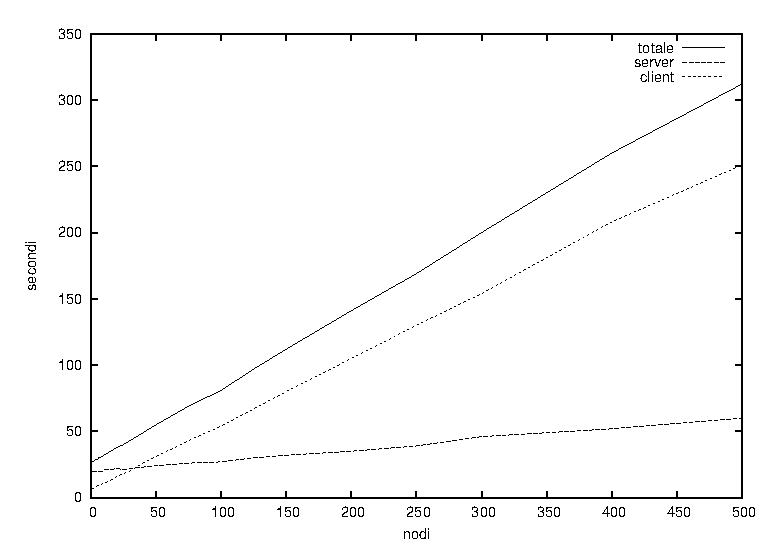
\includegraphics[scale=1.0]{img/qtime.eps}}
\hspace{2.5mm}
\subfigure[risultati su scala logaritmica]
 {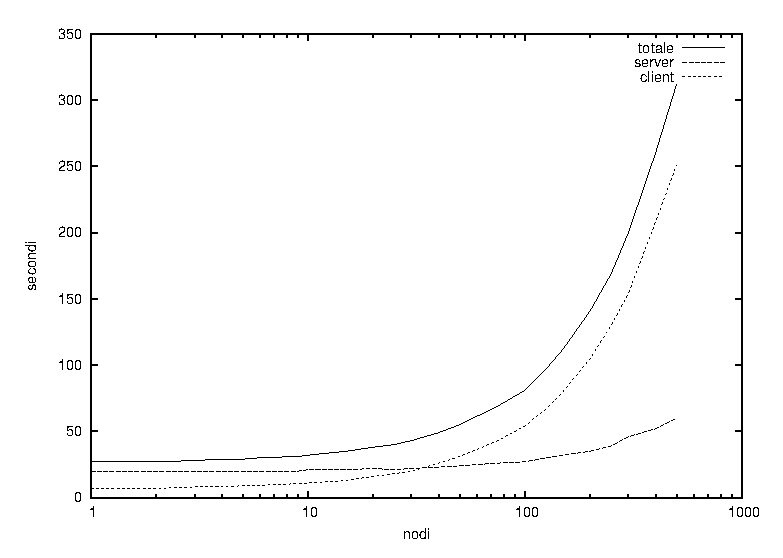
\includegraphics[scale=1.0]{img/qlogtime.eps}}
\caption{\figfont tempi di esecuzione (test distribuito)}\label{fig:qtime}
\end{figure}
Un'analisi del tutto simile pu� essere fatta per il numero di pacchetti e il numero di byte che circolano sulla rete durante le fasi di interazione fra client e server per la risoluzione del problema. In entrambi i casi si ha un comportamento approssimativamente lineare che vede un aumento incontrollato superata una certa soglia, mentre in nessuno dei due si ha una componente costante per quantit� basse di nodi fittizi (cosa del resto prevedibile, visto che anche solo l'aggiunta di un singolo nodo comporta in ogni caso una mole maggiore di dati da scambiare fra le parti).\\
Per quanto riguarda il tempo di trasmissione questo pu� anche non essere preso in considerazione in quanto i test sono stati effettuati su rete LAN e in quasi totale assenza, quindi, di tutti i problemi tipici delle reti estese come la rete Internet, quali la congestione, la caduta di nodi, la variazione sui cammini, etc. Nel caso specifico, il tempo di trasmissione pu� essere recuperato sottraendo dal tempo totale di esecuzione i tempi impiegati lato server e lato client: ci� che rimane rappresenta l'intervallo impiegato per la trasmissione fra le parti. In tutti gli esempi proposti si osserva come questo tempo sia effettivamente trascurabile nel caso specifico.

A questo punto bisogna per� osservare che si pu� considerare il numero di nodi fittizi costante all'interno di un determinato intervallo, ovvero � improbabile che avendo solo dodici nodi intermedi si possano aggiungere addirittura cinquecento nodi fittizi, almeno che lo scopo non sia quello di degradare le prestazioni dell'intero protocollo. Questo si traduce nel fatto che � possibile considerare i risultati ottenuti all'interno di un intervallo di valori approssimativamente compreso fra 10 e 100  nel quale il comportamento di NNSec si pu� approssimare in una componente lineare direttamente dipendente dal numero di nodi coinvolti.\\
Pertanto, approssimando si pu� convalidare l'ipotesi fatta in precedenza, ovvero � possibile considerare praticamente costante il carico in termini di pacchetti e dimensione del flusso per un numero basso di nodi intermedi difficilmente riscontrabile in casi reali, mentre al crescere di tale parametro e mantenendolo all'interno di limiti plausibili le variazioni su tali valori diventano molto pi� apprezzabili e marcate legandosi in modo abbastanza netto al numero di nodi nei livelli intermedi.

Come spesso accade, la teoria si sposa quasi perfettamente con la realt�, anche se deve fare i conti spesso con alcuni aspetti non considerati che portano ad un comportamento leggermente differente. In figura \ref{fig:yxbis} � riportata un'approssimazione dell'andamento di NNSec valida sia in termini di tempo, di nodi e dimensioni del flusso e in cui � messa in evidenza la componente costante e quella che cresce in maniera proporzionale al crescere del numero di nodi appartenenti ai livelli intermedi.

\begin{figure}
\centering
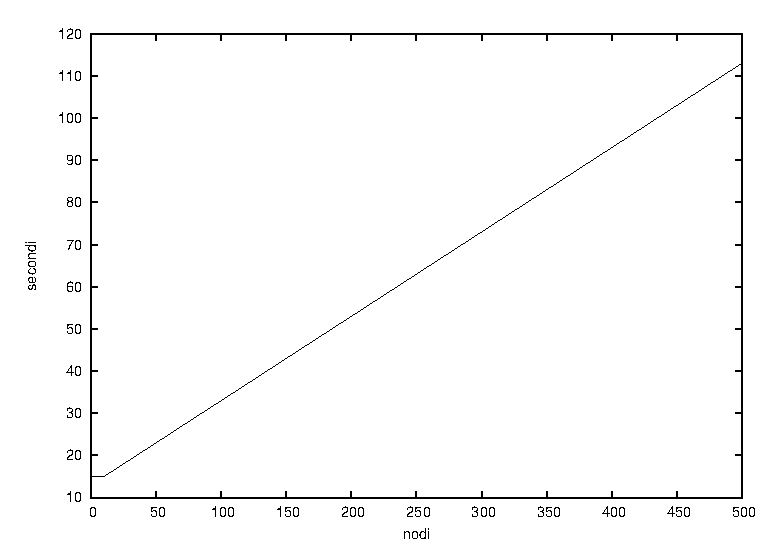
\includegraphics[scale=1]{img/ceil512.eps}
\caption{\figfont approssimazione del comportamento reale}\label{fig:yxbis}
\end{figure}

\paragraph{}
Come era possibile aspettarsi, quindi, dato che l'aggiunta di un nuovo nodo va ad incidere tanto sul numero di nodi che di collegamenti e quindi influisce sia sulla computazione lato server che lato client, questo evento porta ad un innalzarsi dei valori relativi alle prestazioni di NNSec.\\
Quello che � interessante prendere in considerazione � il fatto che se da un lato si ha un carico incidente inevitabile dovuto all'interazione che resta quasi costante anche diminuendo il numero di nodi presenti, dall'altro si ha un comportamento che impone una crescita circa lineare sotto ogni aspetto preso in considerazione una volta superata una certa soglia ed entro certi limiti (in termini di numero di nodi) e che si mantiene tale senza grosse variazioni. Questo permette, senza dubbio, di dare una stima approssimativa di ci� che aspetta l'utente a partire da una determinata configurazione iniziale per la rete neurale.\\
Ovviamente, eventuali congestioni sulla rete o problemi sui nodi (client o server) incidono notevolmente su questa stima e la rendono assolutamente inattendibile, ma del resto niente si pu� contro eventi esterni posti non direttamente sotto il nostro controllo.

Da notare che nell'esempio proposto si hanno sessanta nodi di ingresso, ovvero un carico a priori in termini di tempo, pacchetti e flusso su ogni esempio. Del resto, appunto, questo pu� essere considerato come valore costante e quindi non influisce sul comportamento di NNSec variandolo. I risultati ottenuti possono essere considerati del tutto attendibili e, pertanto, utili ai fini dell'analisi.

\paragraph{}
\begin{table}[ht]
\begin{center}
\begin{tabular}{|c||c|c|c|}
\hline
& \multicolumn{3}{|c|}{\textbf{Fattore di Quantizzazione = 9}} \\
\cline{2-4}
\textbf{Nodi}& \textbf{tempo (s)} & \textbf{client (s)} & \textbf{server (s)} \\
\hline
\hline
12 + 5 & 22 & 2 & 20 \\
12 + 10 & 22 & 2 & 20 \\
12 + 15 & 24 & 3 & 21 \\
12 + 20 & 25 & 4 & 21 \\
12 + 25 & 26 & 4 & 22 \\
12 + 50 & 30 & 7 & 23 \\
12 + 75 & 36 & 10 & 26 \\
12 + 100 & 39 & 12 & 27 \\
12 + 125 & 44 & 14 & 30 \\
12 + 150 & 50 & 17 & 33 \\
12 + 200 & 58 & 23 & 35 \\
12 + 250 & 69 & 28 & 41 \\
12 + 300 & 78 & 33 & 45 \\
12 + 400 & 95 & 44 & 51 \\
12 + 500 & 114 & 55 & 59 \\
12 + 750 & 162 & 81 & 81 \\
12 + 1000 & 208 & 110 & 98 \\
12 + 1250 & 257 & 135 & 122 \\
12 + 1500 & 302 & 164 & 138 \\
\hline
\end{tabular}
\end{center}
\caption{risultati sperimentali (esecuzione locale)}\label{tab:rx64}
\end{table}
Ricollegandosi alla tabella \ref{tab:x64x86}, rappresentata graficamente in figura \ref{fig:qtime}, bisogna mettere in risalto un fatto forse passato inosservato: sebbene per basse quantit� di nodi presenti nella rete neurale il protocollo risulti sbilanciato e il grosso del lavoro sia richiesto al server, aumentando il numero di nodi si ha un punto di incrocio in cui pi� o meno il carico � spartito in modo uguale fra le parti e, incrementando ancora le dimensioni della rete neurale, si nota che il protocollo inizia a pendere verso il client in termini di carico computazionale. In questa situazione, si potrebbe fondare una risposta plausibile basandosi sulla differenza fra le macchine coinvolte e la diversit� delle due architetture; proprio per questo motivo, test simili sono stati effettuati eseguendo sia il client che il server sulla prima delle due macchine descritte in precedenza, cos� da approfondire la questione.\\
\begin{figure}
\centering
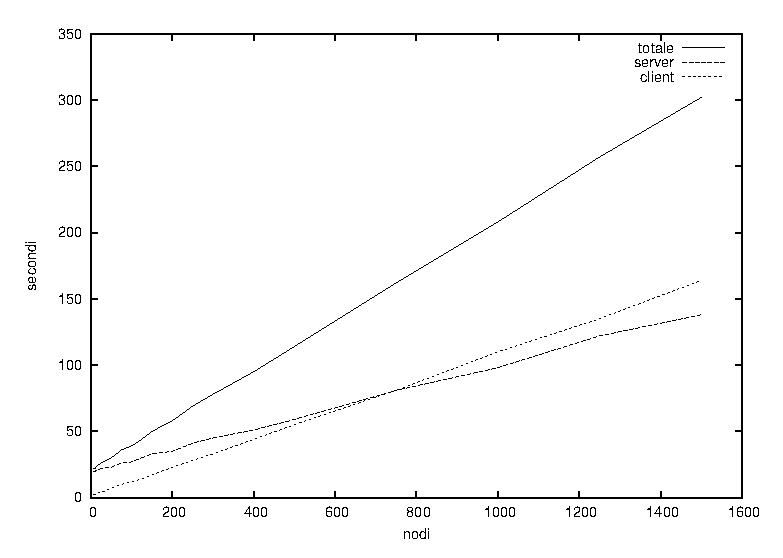
\includegraphics[scale=1.0]{img/qqtime.eps}
\caption{\figfont tempi di esecuzione (test locale)}\label{fig:qqtime}
\end{figure}
I risultati ottenuti sono riportati in tabella \ref{tab:rx64}. La curva ottenuta dai dati cos� ricavati � riportata in figura \ref{fig:qqtime}. Essendo del tutto irrilevanti in casi di esecuzione locale, come quello preso in considerazione, non sono riportati i valori indicanti il numero di pacchetti e la dimensione del flusso dati.

\begin{figure}
\centering
\subfigure[Tempo totale]
 {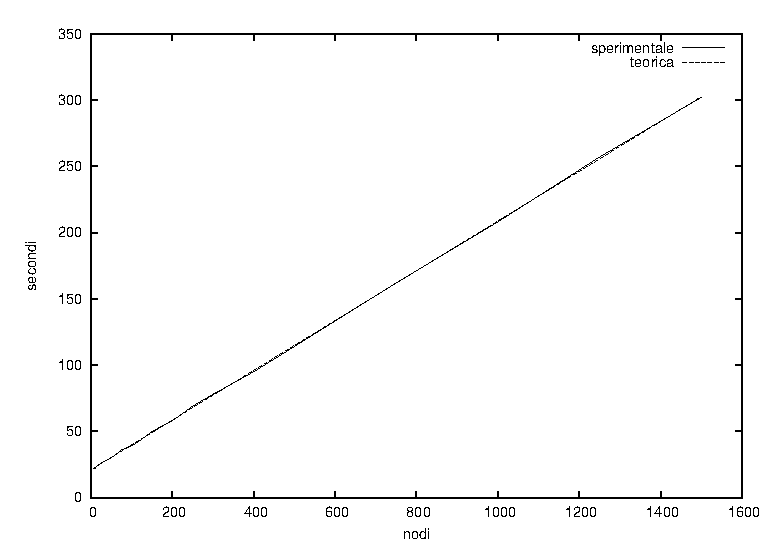
\includegraphics[scale=0.65]{img/bitot.eps}}
\hspace{2.5mm}
\subfigure[Tempo lato server]
 {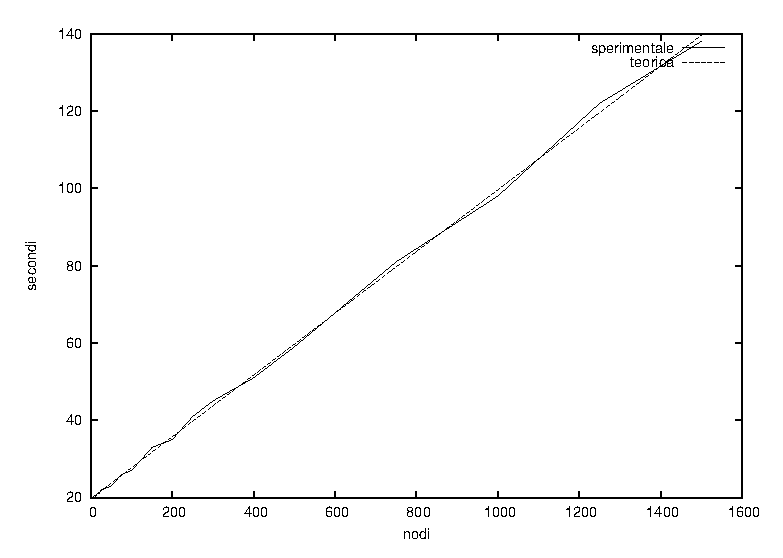
\includegraphics[scale=0.65]{img/biser.eps}}
\hspace{2.5mm}
\subfigure[Tempo lato client]
 {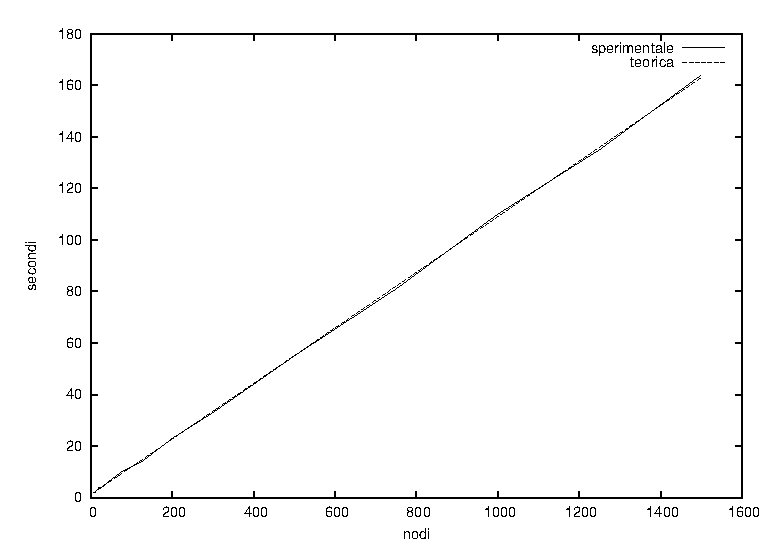
\includegraphics[scale=0.65]{img/bicli.eps}}
\caption{\figfont Approssimazione del comportamento temporale}\label{fig:bifig}
\end{figure}

Anche in questo caso si nota come al crescere del numero di nodi presenti nella rete neurale le prestazioni lato client peggiorino, a tal punto da eguagliare il comportamento lato server fino a superarlo in termini di tempo di esecuzione. Le curve ottenute dai dati sperimentali possono essere approssimate con delle rette, come riportato in figura \ref{fig:bifig} dove sono evidenziati rispettivamente i casi del tempo totale impiegato (figura \ref{fig:bifig} \textit{(a)}), del tempo lato server (figura \ref{fig:bifig} \textit{(b)}) e del tempo impiegato sul client (figura \ref{fig:bifig} \textit{(c)}).\\
Le rette ottenute possono essere descritte nella forma intercetta/coefficiente angolare, ovvero: $ y = mx + q $. Dai dati in possesso, attraverso una operazione di approssimazione con il metodo dei minimi quadrati, si ottengono le coppie di parametri di seguito riportate:
\begin{itemize}
 \item Tempo totale:
  \begin{itemize}
   \item intercetta: 20.98300
   \item coefficiente angolare: 0.18771
  \end{itemize}
 \item Tempo impiegato sul server:
  \begin{itemize}
   \item intercetta: 19.790616
   \item coefficiente angolare: 0.079848
  \end{itemize}
 \item Tempo impiegato sul client:
  \begin{itemize}
   \item intercetta: 1.19238
   \item coefficiente angolare: 0.10786
  \end{itemize}
\end{itemize}
Nello specifico, la tecnica di approssimazione dei minimi quadrati tenta di approssimare una funzione che si avvicini quanto pi� possibile alla funzione ottenuta dall'interpolazione dei punti considerati, ma che non necessariamente passi attraverso di essi. In particolare, si cerca di minimizzare il valore indicato come: $ S = \sum^n_{i=1}\left(y_i-f\left(x_i\right)\right)^2 $, dove sia $ n $ il numero di coppie $ \left(x_i, y_i\right) $ considerate. Questo consiste nel minimizzare il quadrato delle distanze fra i punti $ y_i $ e $ f\left(x_i\right) $, da cui il nome del metodo. Nel caso specifico dell'approssimazione di una retta, data la forma: $ y = f\left(x\right) = mx + q $, il problema si riduce all'approssimazione dei parametri $ m $ e $ q $, ovvero il coefficiente angolare e l'intercetta. Date $ n $ coppie $ \left(x_i, y_i\right) $, si ricavano come segue:
$$ m = \frac{\sum{x_i}\cdot\sum{y_i} - n\sum{x_iy_i}}{\left(\sum{x_i}\right)^2 - n\sum{\left(x_i\right)^2}} $$
$$ q = \frac{\sum{x_i}\cdot\sum{\left(x_iy_i\right)} - \sum{\left(x_i\right)^2}\sum{y_i}}{\left(\sum{x_i}\right)^2 - n\sum{\left(x_i\right)^2}} $$

Il comportamento adottato dalle diverse curve segue dal numero crescente di richieste di servizi verso il client da parte del server, in quanto per ogni nodo � richiesta una elaborazione che consiste in una fase di decifratura, elaborazione di dati e conseguente nuova cifratura, fasi che intuitivamente e inevitabilmente incidono sulle prestazioni lato client data la loro complessit�.\\
Nonostante esplicitare una formula precisa per via analitica non sia cosa immediata data la presenza di una vastit� di fattori da prendere in considerazione (come ad esempio il costo di una moltiplicazione o di un elevamento a potenza, cos� come i ritardi introdotti dalla \textit{Java Virtual Machine} e tanto altro ancora) si nota come le fasi di cifratura e decifratura risultino pi� costose rispetto ad operazioni di moltiplicazione o elevamento a potenza, seppure anche quest'ultime vengano portate avanti con valori aventi lunghezza media pari a 1024 bit. Questo lo si pu� dedurre dal fatto che le prestazioni del client peggiorano molto pi� velocemente rispetto a quelle del server proprio al crescere del numero di nodi (bisogna infatti considerare che per ogni nodo intermedio aggiuntivo il client � soggetto ad una fase di decifratura e conseguente cifratura aggiuntiva durante l'elaborazione dei risultati).\\
Ancora, sebbene una stima a priori discenda necessariamente dai parametri sopra citati e non possa essere espressa in maniera precisa ed univoca per ogni singolo caso indipendente, si pu� osservare come la crescita sia lineare con il numero di nodi e permetta di effettuare effettivamente una predizione sul comportamento di una data macchina a partire da pochi esempi di esecuzione.

\paragraph{}
Alla luce di quanto detto si pu� dire che le osservazioni fatte in precedenza mantengono ancora la loro validit� sebbene, di contro, lo sbilanciamento lato client che si presenta al crescere del numero di nodi nella rete neurale porta ad un allungamento notevole dei tempi di risoluzione nel caso in cui la macchina su cui viene eseguita la parte client non permetta prestazioni elevate. Questo preclude l'uso di software basato sul protocollo proposto con macchine datate e non molto performanti. Del resto bisogna dire che il punto di incrocio che rappresenta una situazione in cui il carico � spartito in modo uguale fra client e server � strettamente dipendente dalle macchine coinvolte e, in ogni caso, reti che presentano un basso numero di nodi intermedi (sia reali che fittizi) possono essere messe a disposizione anche di client dalle prestazioni inferiori, ammesso che questi abbiano sufficiente pazienza fra le proprie caratteristiche.


\backmatter
\chapter{Appendice A}
In questa appendice viene indicato l'insieme dei simboli riconosciuti da NNSec e la grammatica utilizzata per la descrizione delle reti neurali. Essendo stati utilizzati i programmi JavaCUP e JFlex e avendo questi una sintassi particolare, viene in realt� riportata parte del contenuto dei file sottomessi come ingressi ai programmi sopra citati. Per maggiori informazioni, � consigliato fare riferimento alla documentazione ufficiale dei due programmi sopra citati.

\paragraph{Simboli Terminali}
I simboli basilari, su cui sono costruiti mattone dopo mattone tutti gli altri, sono i seguenti:
\begin{lstlisting}
  nl  =  [\r|\n|\r\n]*
  ws  =  [ \t\f]*
  wtok  =  {nl} | {ws}
  equal  =  {ws}"="{ws}
  sfloat  =  ["+"|"-"]?[0-9]+"."[0-9]*
  integer  =  [0-9]+
  string  =  [a-zA-Z0-9 ]+
  lbracket  =  {wtok}"{"{wtok}
  rbracket  =  {wtok}"}"{wtok}
  endterm	  =  {wtok}";"{wtok}
\end{lstlisting}
A partire da questi, lo spazio di valutazione � diviso in sezioni e alcuni simboli composti possono apparire solo in alcune aree mentre altri assumono significati diversi a seconda dell'area in cui si presentano. L'area principale, dalla quale comincia la valutazione, e i simboli in essa possibili sono di seguito riportati:
\begin{lstlisting}
  <YYINITIAL>
    NET_SEC : "net"{lbracket}
\end{lstlisting}
Quanto sopra impone decisamente che la descrizione relativa ad una rete neurale inizi con il termine \textit{net} seguito da una parentesi graffa aperta, nessun altro termine � accettato. L'unico valore possibile definisce anche la seconda area di valutazione, composta come sotto indicato:
\begin{lstlisting}
  <NET_SEC>
    NAME : "name"{equal}
    DESC : "description"{equal}
    ACTVF : "actv"{equal}
    OUTF : "out"{equal}
    O_NODE_SEC : ["output"{lbracket}|"onode"{lbracket}]
    I_NODE_SEC : ["input"{lbracket}|"inode"{lbracket}]
    H_NODE_SEC : ["hidden"{lbracket}|"hnode"{lbracket}]
    LINK_SEC : "link"{lbracket}
    STRING : {string}
    END_TERM : {endterm}
    NET_SEC_END : {rbracket}
\end{lstlisting}
Le sezioni che seguono direttamente da quella sopra introdotta sono relative ai nodi di ingresso, nodi di uscita e nodi nascosti (ovvero appartenneti ai livelli intermedi) e ai collegamenti presenti fra nodi, rispettivamente.\\
La prima delle sezioni � relativa ai nodi di ingresso:
\begin{lstlisting}
  <I_NODE_SEC>
    NODE_ID : "id"{equal}
    ID_VALUE : {integer}
    END_TERM : {endterm}
    NODE_SEC_END : {rbracket}
\end{lstlisting}
La seconda � invece relativa ai nodi nascosti, o intermedi:
\begin{lstlisting}
  <H_NODE_SEC>
    NODE_ID : "id"{equal}
    ACTVF : "actv"{equal}
    OUTF : "out"{equal}
    GROUP_ID : ["layer"{equal}|"group"{equal}]
    THRESHOLD : "threshold"{equal}
    THRESHOLD_VALUE : {sfloat}
    ID_VALUE : {integer}
    STRING : {string}
    END_TERM : {endterm}
    NODE_SEC_END : {rbracket}
\end{lstlisting}
La terza, ancora, � relativa ai nodi di uscita:
\begin{lstlisting}
  <O_NODE_SEC>
    NODE_ID : "id"{equal}
    ACTVF : "actv"{equal}
    OUTF : "out"{equal}
    THRESHOLD : "threshold"{equal}
    THRESHOLD_VALUE : {sfloat}
    ID_VALUE : {integer}
    STRING : {string}
    END_TERM : {endterm}
    NODE_SEC_END : {rbracket}
\end{lstlisting}
Infine, la sezione riguardante i collegamenti fra nodi:
\begin{lstlisting}
  <LINK_SEC>
    LINK_INPUT_NODE_ID : ["to"{equal}|"hnode"{equal}]
    LINK_OUTPUT_NODE_ID : ["from"{equal}|"tnode"{equal}]
    LINK_WEIGHT : "weight"{equal}
    WEIGHT_VALUE : {sfloat}
    NODE_ID_VALUE : {integer}
    END_TERM : {endterm}
    LINK_SEC_END : {rbracket}
\end{lstlisting}

\paragraph{Grammatica}
La grammatica per la costruzione di reti neurali � di seguito riportata e si basa sui simboli discussi nella sezione precedente. Questa � volutamente semplice ma completa e permettere di descrivere potenzialmente qualsiasi tipo di rete neurale, con le dovute limitazioni in base alle reti ``comprese'' da NNSec. I simboli terminali sono riportati in lettere maiuscole, i simboli non terminali in lettere minuscole.
\begin{lstlisting}
  net_list  ::=  net_list net_expr
                 | net_expr

  net_expr  ::=  NET_SEC net_tokens node link NET_SEC_END

  net_tokens  ::=  net_tokens net_token
                   | net_token

  net_token  ::=  name
                  | desc
                  | actvfunc
                  | outfunc

  name  ::=  NAME STRING END_TERM

  desc  ::=  DESC STRING END_TERM

  actvfunc  ::=  ACTVF STRING END_TERM

  outfunc  ::=  OUTF STRING END_TERM

  node  ::=  node node_expr
             | node_expr

  node_expr  ::=  inode
                  | hnode
                  | onode

  inode  ::=  I_NODE_SEC node_tokens NODE_SEC_END

  hnode  ::=  H_NODE_SEC node_tokens NODE_SEC_END

  onode  ::=  O_NODE_SEC node_tokens NODE_SEC_END

  node_tokens  ::=  node_tokens node_token
                    | node_token

  node_token  ::=  gid
                   | id
                   | nodeactvfunc
                   | nodeoutfunc
                   | threshold

  gid  ::=  GROUP_ID ID_VALUE END_TERM

  id  ::=  NODE_ID ID_VALUE END_TERM

  nodeactvfunc  ::=  ACTVF STRING END_TERM

  nodeoutfunc  ::=  OUTF STRING END_TERM

  threshold  ::=  THRESHOLD THRESHOLD_VALUE END_TERM

  link  ::=  link link_expr
             | link_expr

  link_expr  ::=  LINK_SEC output_ref \
                        input_ref weight LINK_SEC_END

  input_ref  ::=  LINK_INPUT_NODE_ID NODE_ID_VALUE END_TERM

  output_ref  ::=  LINK_OUTPUT_NODE_ID NODE_ID_VALUE END_TERM

  weight  ::=  LINK_WEIGHT WEIGHT_VALUE END_TERM
\end{lstlisting}
\paragraph{}
Grazie alla grammatica utilizzata, descrivere le reti neurale diventa facile e intuitivo per chiunque. Inoltre, per come � stata concepito, NNSec permette di inserire pi� reti neurali in un unico file se si ritiene utile.\\
Insieme al software sono distribuite alcune reti neurali \textit{di prova}, che possono essere utilizzate per testare client e server e dare un'idea di come questi file devono essere effettivamente scritti. Di seguito, un esempio di rete neurale descritta grazie alla grammatica sopra citata:
\begin{lstlisting}
  net {
    name = seno;
    description = ritorna il seno del valore;
    actv = sigmoid;
    inode { id=0; }
    hnode { id = 1; layer = 1; threshold = -2.1814; }
    hnode { id = 2; layer = 1; threshold = -10.9423; }
    hnode { id = 3; layer = 2; threshold = -1.5133; }
    hnode { id = 4; layer = 2; threshold = -2.9522; }
    onode { id = 5; threshold = 0.5348; }
    link { from = 0; to = 1; weight = 3.7558; }
    link { from = 0; to = 2; weight = 12.2071; }
    link { from = 0; to = 3; weight = 14.5007; }
    link { from = 0; to = 4; weight = -2.0168; }
    link { from = 1; to = 5; weight = -13.1986; }
    link { from = 2; to = 5; weight = 6.8320; }
    link { from = 3; to = 5; weight = 5.0785; }
    link { from = 4; to = 5; weight = -1.9914; }
  }
\end{lstlisting}
In tabella \ref{tab:sin} sono riportati i valori associati alla rete neurale riportata. In realt�, questa rete prende come ingressi valori compresi fra 0 e 1 che rappresentano l'angolo tra 0 e 360 gradi, mentre in uscita forniscono il seno dell'angolo nel range $ 0,1 \dots 0,9 $  (il valore da $ 0,1 $ a $ 0,9 $ in uscita deve rappresentare il seno da $ -1 $ a $ +1 $).
\begin{table}[t]
\begin{center}
\begin{tabular}{|c|c|c|c|}
\hline
\textbf{Gradi} & \textbf{Seno} & \textbf{Ingressi} & \textbf{Uscite} \\
\hline
0.0 & 0.0000 & 0.0000 & 0.5000 \\
22.5 & 0.3827 & 0.0625 & 0.6531 \\
45.0 & 0.7071 & 0.1250 & 0.7828 \\
67.5 & 0.9239 & 0.1875 & 0.8696 \\
90.0 & 1.0000 & 0.2500 & 0.9000 \\
112.5 & 0.9239 & 0.3125 & 0.8696 \\
135.0 & 0.7071 & 0.3750 & 0.7828 \\
157.5 & 0.3827 & 0.4375 & 0.6531 \\
180.0 & 0.0000 & 0.5000 & 0.5000 \\
202.5 & -0.3827 & 0.5625 & 0.3469 \\
225.0 & -0.7071 & 0.6250 & 0.2172 \\
247.5 & -0.9239 & 0.6875 & 0.1304 \\
270.0 & -1.0000 & 0.7500 & 0.1000 \\
292.5 & -0.9239 & 0.8125 & 0.1304 \\
315.0 & -0.7071 & 0.8750 & 0.2172 \\
337.5 & -0.3827 & 0.9375 & 0.3469 \\
360.0 & 0.0000 & 1.0000 & 0.5000 \\
\hline
\end{tabular}
\end{center}
\label{tab:sin}
\end{table}
\paragraph{}
Una nota in particolare va fatta sulla flessibilit� implicita, propria di molti linguaggi, che permette di fare cose al di l� di ci� per cui sono stati concepiti grazie a qualche trucco o forzatura delle regole di base. Questo � anche il caso della grammatica introdotta in NNSec. Un esempio molto semplice � la possibilit� di aggiungere implicitamente nodi di bias senza doverli descrivere in modo indipendente, semplicemente ponendo il valore del collegamento associato come soglia del nodo a cui fanno riferimento. Infatti, sia $ t $ la soglia, questa � aggiunta al valore computato per il singolo nodo considerandola come il peso di un collegamento stabilito da un nodo unitario: proprio lo stesso modo in cui viene considerato il valore di bias!\\
Basta lasciar correre la fantasia e anche con la grammatica utilizzata in NNSec, sposata con la struttura del codice, si possono trovare tanti altri trucchi per aggirare problemi o risolvere in modo veloce ed efficiente varie questioni.

\chapter{Appendice B}
L'interfaccia grafica � una componente importante per quanto riguarda l'interazione con il software. Nel caso di NNSec, questa si suddivide in due componenti e mette a disposizione lato server un metodo per configurare il sistema e caricare nuove reti neurali in modo da metterle a disposizione di utenti remoti, mentre per i client sono disponibili controlli veloci ed intuitivi per il recupero della lista di reti neurali disponibili e l'uso di quest'ultime. Inoltre, in entrambi i casi � presente un'area di log in cui sono riportati dati utili o informazioni sommarie in caso di eventuali errori.\\
Brevemente, saranno descritte nel seguito le interfacce grafiche lato client e lato server e come queste possono essere utilizzate per interagire con NNSec a seconda dei casi.

\paragraph{Interfaccia lato client.}
Per quanto riguarda il client, l'interfaccia grafica � concepita per permette all'utente una connessione remota verso un server NNSec, il recupero della lista di reti neurali disponibili su di esso e quindi l'uso di quest'ultime.\\
\begin{figure}[ht]
\centering
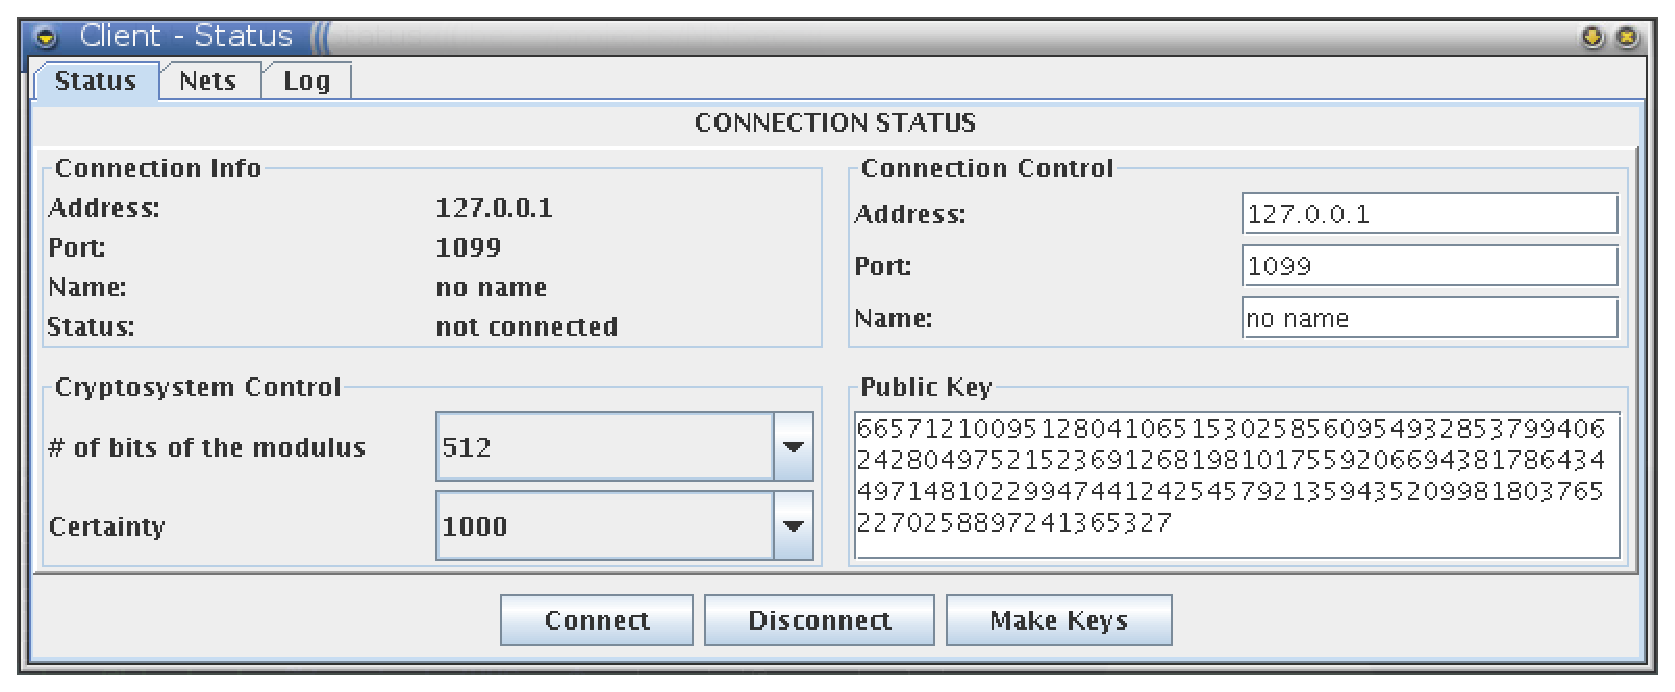
\includegraphics[scale=0.45]{img/cstat.eps}
\end{figure}
Tramite il pannello \textit{status} � possibile indicare l'indirizzo IP del server desiderato e quindi la porta su cui effettuare la connessione, oltre al nome del server che si vuole contattare. Nello stesso pannello sono riportati dati riguardanti la connessione stessa, come ad esempio il fatto che essa sia attiva o meno. Ancora, dal pannello di status � possibile gestire la propria chiave pubblica impostandone a piacere i parametri e generandone di nuove ogni volta che lo si desidera, con la possibilit� di consultazione.\\
\begin{figure}[ht]
\centering
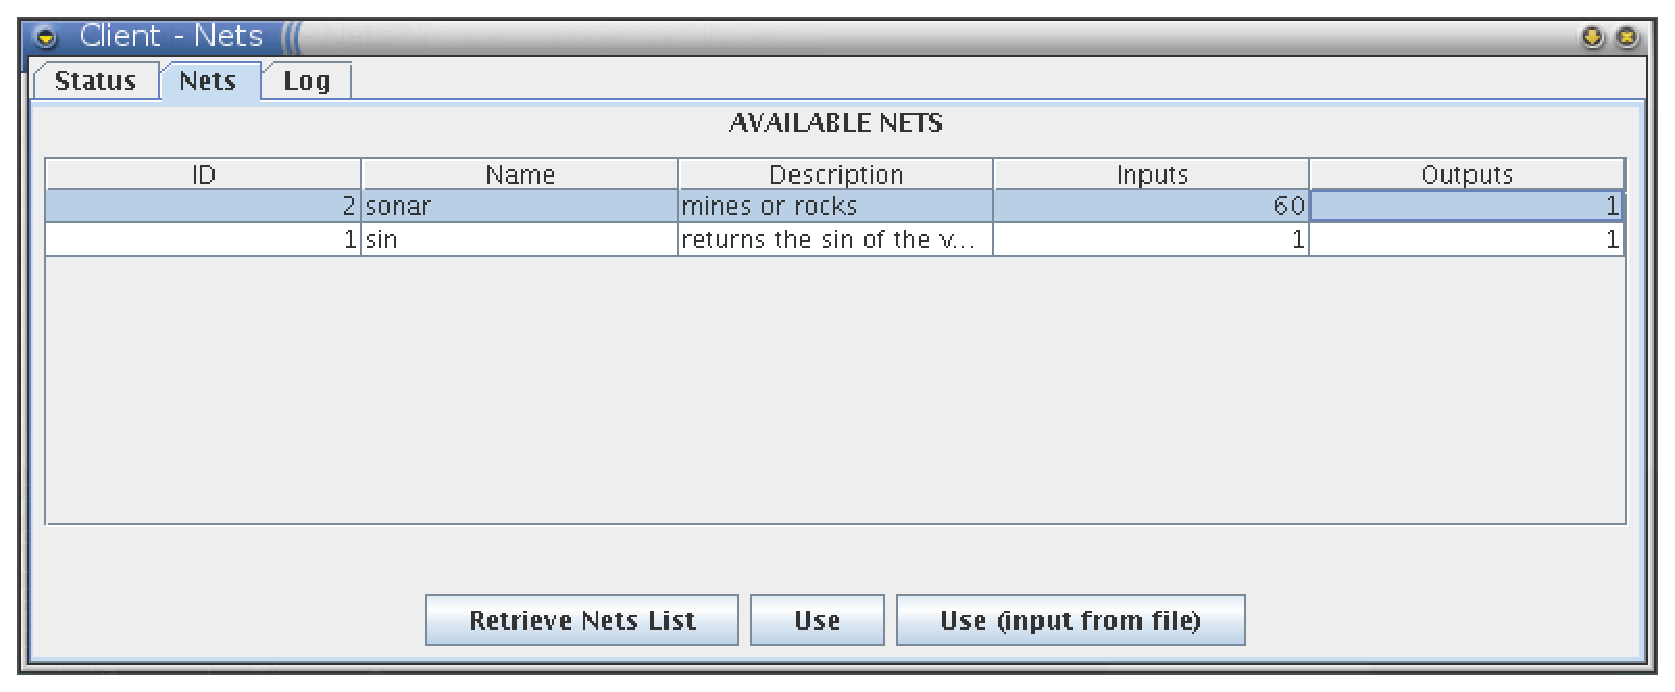
\includegraphics[scale=0.45]{img/cnets.eps}
\end{figure}
Dal pannello \textit{Nets} si pu� procedere al recupero e l'uso delle reti neurali. Una volta stabilita la connessione, infatti, tramite quest'area si pu� accedere alle reti neurali disponibili scaricandone una lista dal server e quindi procedere all'uso di una di queste tramite l'inserimento manuale dei dati di ingresso o, nei casi in cui questo risulta scomodo a causa della loro mole, facendo leggere i dati di ingresso direttamente da un file di ingresso sul quale questi dovranno apparire in numero di uno per riga.\\
\begin{figure}[ht]
\centering
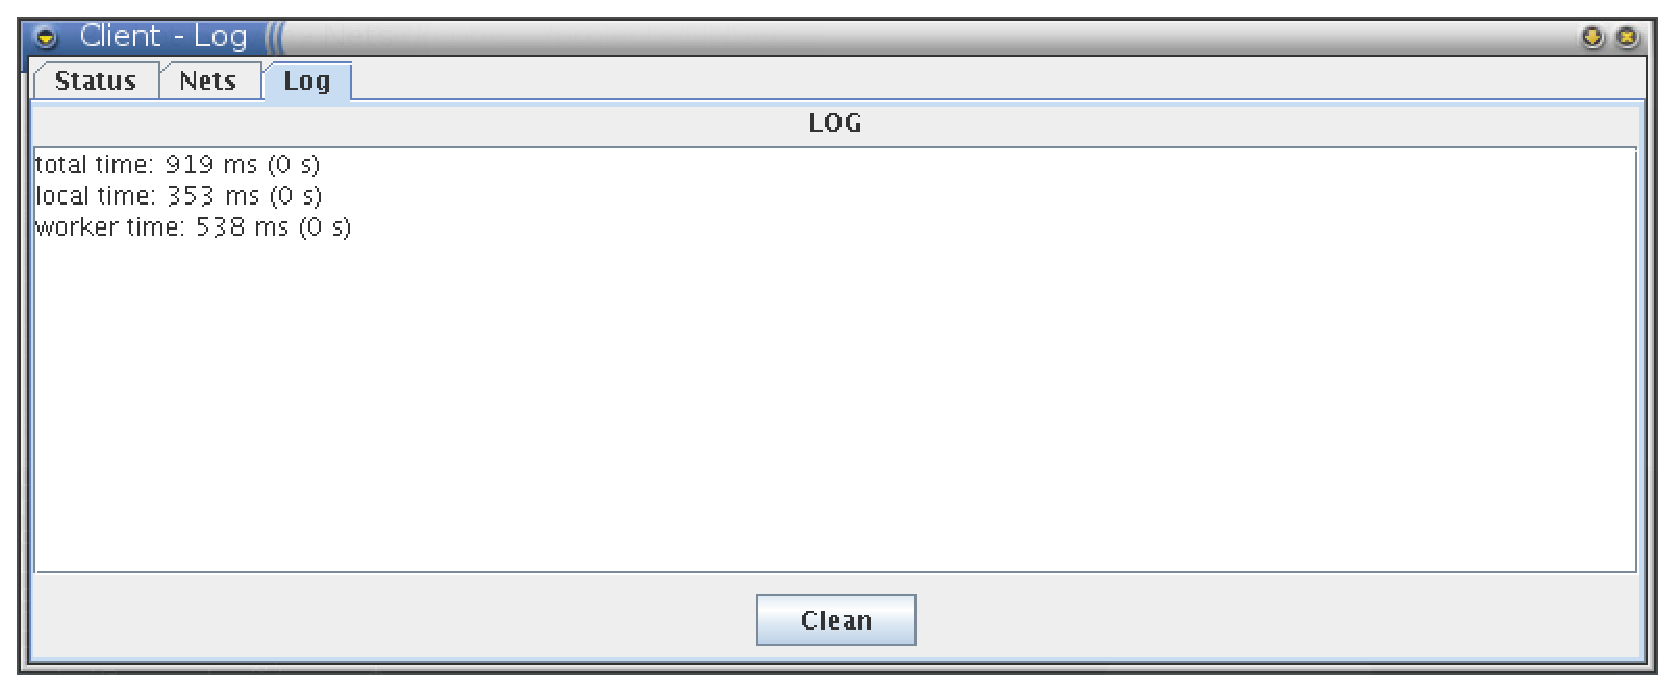
\includegraphics[scale=0.45]{img/clog.eps}
\end{figure}
In caso di errori durante la connessione ad un server o l'uso di una rete neurale, oppure addirittura in caso di errori interni al programma, nell'area di \textit{log} si pu� ottenere una breve descrizione dell'errore per cercare di capire a cosa sia dovuto il problema. Lato client, inoltre, in questa zona sono riportati dati descrittivi riguardanti la singola sessione d'uso di una rete neurale, ovvero � indicato in modo approssimativo il tempo di elaborazione totale, quello impiegato sul server e quello impiegato sul client, dai quali � poi possibile ricavare il tempo perso nelle fasi di trasmissione dei dati.

\paragraph{Interfaccia lato server.}
\begin{figure}[ht]
\centering
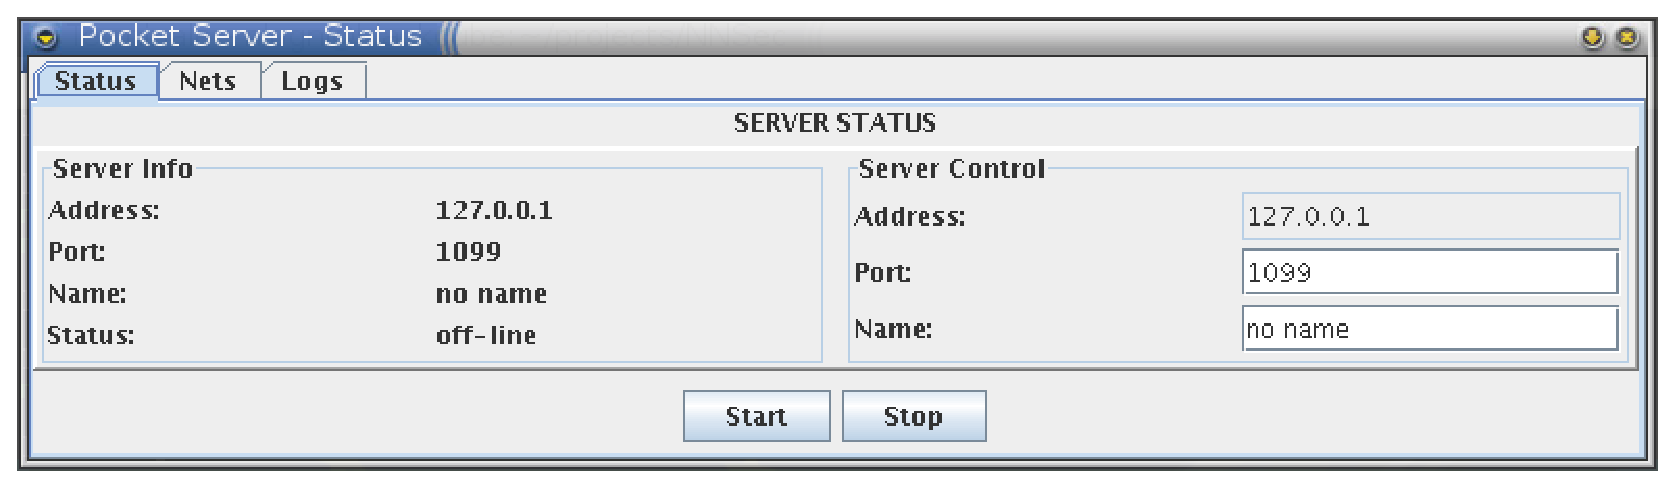
\includegraphics[scale=0.45]{img/sstat.eps}
\end{figure}
L'interfaccia grafica del server mette a disposizione metodi e campi per aggiungere nuove reti neurali al sistema, impostarne i parametri e renderle disponibili per gli utenti remoti. Questo �, senza dubbio, lo scopo primario del server e quindi deve risultare quanto pi� facile, flessibile e intuitivo possibile.\\
\begin{figure}[ht]
\centering
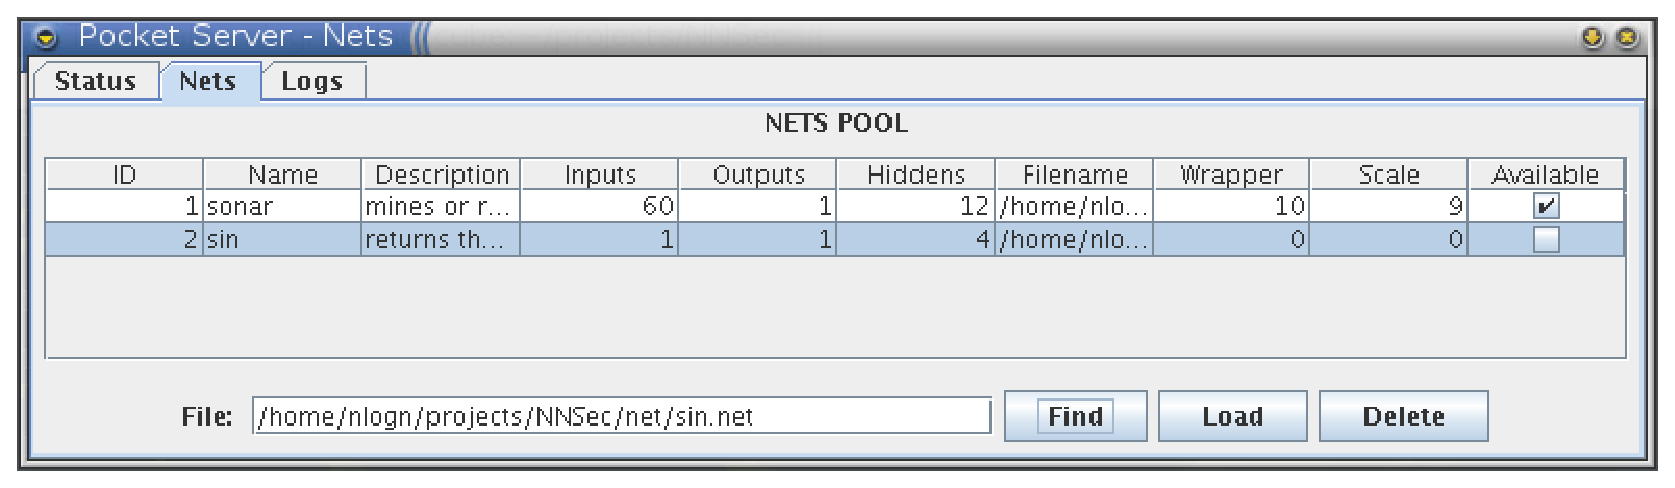
\includegraphics[scale=0.45]{img/snets.eps}
\end{figure}
Il pannello \textit{status} permette di gestire alcuni parametri relativi al server quali la porta su cui questo dovr� ascoltare e il nome a cui dovr� rispondere, in base alle chiamate. Da osservare che, in realt�, questi parametri sono relativi al registro rmi che fornir� ai client il riferimento al server NNSec (riferimento che, effettivamente, � associato al nome indicato in questo pannello). Come nel caso del pannello \textit{status} presente sul client, anche lato server sono riportati parametri relativi la connessione, come ad esempio il suo stato.\\
\begin{figure}[ht]
\centering
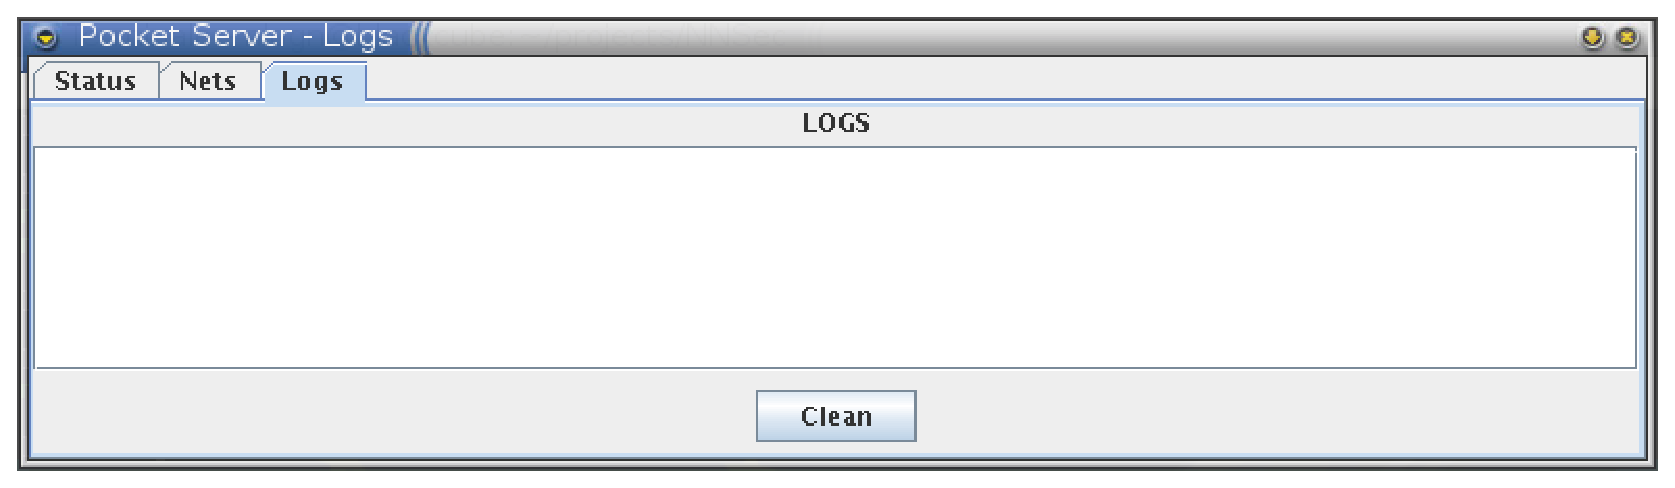
\includegraphics[scale=0.45]{img/slog.eps}
\end{figure}
Il pannello \textit{Nets} rappresenta il cuore della gestione delle reti neurali, ovvero il modo attraverso il quale l'utente pu� interagire e configurare tali elementi. Come si pu� notare � possibile caricare (ricercando sul filesystem il file di descrizione apposito) nuove reti neurali nel sistema, quindi associare ad ognuna di loro in modo indipendente un fattore di quantizzazione appropriato e il numero desiderato di nodi fittizi associati. Infine, tramite questo pannello � possibile decidere quali reti neurali risulteranno disponibili o meno agli utenti remoti.\\
Nell'area di \textit{log} sono riportati messaggi di errore interni al sistema. Esempi di queste situazioni di errore sono l'impossibilit� di effettuare il parsing dei file di descrizione per le reti neurali, l'incapacit� di creazione del registro di nomi per rmi e l'associazione quindi del riferimento locale o anche errori specifici del programma come, ad esempio, la mancanza di determinate classi laddove queste siano state cancellate per errore.

\chapter{Conclusioni}
Dall'idea alla realizzazione concreta di un protocollo. Da un'idea allo studio di nuovi terreni dove fino ad oggi la crittografia non si era mai spinta. Dall'idea al prodotto finale, un punto di partenza e non di arrivo.
\paragraph{}
Lo sviluppo di un protocollo concepito e approfondito solamente in linea teorica pu� nascondere molte sorprese e raramente rappresenta un percorso facile e privo di problemi. Ci� nonostante, questo cammino pu� giovare anche all'idea da cui tutto � partito, come nel caso di NNSec e del protocollo implementato. Da un concetto ad un insieme di classi, interfacce e relazioni fra queste il passo � breve, ma dove alcuni nodi si sciolgono in maniera pi� facile del previsto, altri vengono al pettine e rischiano di dare molti grattacapi. Da una teoria ad un algoritmo, la via � corta ma a volte tortuosa.\\
L'implementazione del protocollo ha richiesto l'applicazione di molte tecniche e tecnologie, come dimostrazione di quanto alcuni concetti di teoria apparentemente banali si rivelino fondamentali quando sposati con altri concetti, a loro volta tanto innocui quanto inaspettatamente utili. Dalla teoria alla pratica, � stato dimostrato che il protocollo proposto pu� essere ``tradotto'' in un insieme di elementi che, interagendo fra di loro, concorrono ad implementare quanto ipotizzato.

\paragraph{}
Ma non solo.

Passando da un'idea al codice, � stato dimostrato che le prestazioni non sono cos� pessime e queste possono ancora migliorare utilizzando altri linguaggi e diverse tecniche. Ancora, � stato osservato che l'utilizzo di reti neurali remote � uno scenario plausibile, il che comporta la validit� e attualit� del protocollo proposto.\\
La possibilit� di realizzare soluzioni concrete in questo ambito viene quindi avvalorata dalla possibilit� di avere prestazioni decorose, non drasticamente pessime o assolutamente inaccettabili. Senza dubbio, i limiti della crittografia in termini di calcolo computazionale (ancora oggi non superati e non superabili) incidono sui tempi impiegati dal prodotto finale per giungere ad un risultato partendo dagli ingressi, ma le risposte ottenute in fase sperimentale hanno dato buone speranze e dipingono un futuro roseo per le applicazioni di crittografia in questo campo.

\paragraph{}
Senza dubbio, a partire dal protocollo, passando per il lavoro di tesi e arrivando al prodotto finale, rappresentato dal software NNSec, si deduce che questo ambito in cui la crittografia fino a poco tempo fa era solo una leggenda oggi pu� rappresentare un terreno di studio fertile e pieno di sorprese. Le reti neurali possono essere sposate con un cifrario che presenti determinate caratteristiche e possono essere utilizzate in sicurezza, sia dal punto di vista dell'utente che del fornitore. L'avvento di nuove tecnologie e nuove tecniche, sia nell'ambito della crittografia che in quello delle reti neurali, unito ai passi avanti fatti da compilatori e linguaggi possono lasciare spazio a prestazioni migliori per il futuro e convalidano, senza dubbio, l'ipotesi per cui questa strada non sia da abbandonare ma bens� da percorrere fino in fondo.

Come detto, questo lavoro di tesi rappresenta senza dubbio non un punto di arrivo con il software implementato, ma un punto di partenza con i dati ricavati da tale software, i quali dimostrano che la strada � tutt'altro che senza via d'uscita.
\bibliography{bib}
% blank-page
\thispagestyle{empty}
\hbox{\hspace{1in}}
\newpage
% / blank-page
\chapter{Ringraziamenti}

Seduto sul letto di Casa Terronia ho finito di scrivere, di leggere, di rileggere la mia tesi e aspetto solo che i \textit{critici} mi facciano avere le loro revisioni \dots \texttt{Non mi sembra vero!} E visto che la voglia di studiare manca, quale momento migliore per qualche ringraziamento? Da vero informatico andr� in ordine sparso ma consigliando l'uso di un algoritmo per l'ordinamento di questa pagina con complessit� $ O(N\ln N) $.

\paragraph{}
Per�, quanti siete ...

\paragraph{}
Tre anni fa � iniziata l'avventura e i primi che devo ringraziare sono i miei genitori, il mio vecchio e consorte, perch� se non ci credevamo n� io n� voi in fondo ci speravamo tutti un po' che avessi davvero messo la testa a posto. E oggi, guardate qua \dots \textit{Grazie di cuore, grazie di tutto, grazie davvero!} Questo sogno si realizza anche e soprattutto grazie a voi! Sono costoso, forse, ma almeno ne vale la pena (spero)!? Grazie ai miei \texttt{fratelli} e alla mia \texttt{gemellina}, cosa sarei senza di voi: un figlio unico viziato a cui non manca niente, se non due fratelli e una gemellina che non cambierei per niente al mondo. Grazie anche ai \texttt{``parenti acquisiti''}, a tutti quelli che in \textit{Puglia} ogni tanto mi pensano, a tutti quelli che Estate dopo Estate mi accolgono e mi fanno sentire a casa, mi fanno sentire bene. Grazie davvero.

Grazie anche ai miei \textit{amici}, ma non a quelli che si ricordano di me solo quando mi vedono al bar, piuttosto a quelli che si ricordano di me proprio quando non mi vedono al bar!!

Grazie a tutti i \textit{compagni di viaggio} di quest'avventura che � l'universit�, ai \textbf{vecchi} e ai \textbf{nuovi}. Grazie a Droscy e a un amico che spero non perder� mai (chiss� quando mi sarei laureato, senza di te), a Fox e ai suoi problemi idilliaci (quante ore, quante litigate, quante risate), al Booga a cui non ho mai detto grazie per avermi strappato una risata anche all'ospedale mentre piangevo il mio naso rotto, a Trevi\~{n}o (e la sua \~{n} che ci vuole proprio una laurea in ingegneria per digerirla) e a Paolo, il Paolo che ci ha abbandonati, il Paolo del Romito, il Paolo di Geometria e Algebra Lineare, il Paolo che \underline{non � meteora}, il Paolo con cui ho condiviso un primo, splendido anno. Grazie poi a tutti quelli che hanno cominciato con me e incrociato il mio cammino anche solo per un attimo. Ma si, ma si, non mi sono dimenticato, grazie anche alla bionda e al rame: vi ho conosciuti tardi ma meglio tardi che mai, no? E grazie a GJ, un amico a cui avrei potuto chiedere tanto (viste le doti) ma a cui non ho chiesto niente, perch� amico e non miniera d'oro. Grazie agli ultimi arrivati, poi, soprattutto al signor \texttt{rappresentante degli studenti} con cui ho condiviso l'esperienza tesi: ma quante risate ci siamo fatti mentre fuori pioveva? Ultimo, ma non ultimo, chi mi ha prestato i suoi appunti, dato i suoi consigli, accettato come amico non solo nel momento del bisogno quando ho teso la mano ma anche dopo, quando poteva andarsene: � bello sapere che c'� ancora gente cos�, gente che arriva sempre \textit{Just-in Time}!

Ma l'universit� non sono solo \texttt{studenti}, anche \texttt{professori}! Ovviamente grazie ad Alessandro\footnote{\#define Alessandro professore} (aka professor Piva) per avermi accolto nella sua ``famiglia'' e dato la libert� di cui avevo bisogno, e grazie anche a tutto il \texttt{laboratorio comunicazioni e immagini}. Grazie a Claudio perch� mi ha risposto quando neanche sapeva chi fossi e ha continuato a farlo anche dopo averlo scoperto! Grazie pure al professor Luchetta, perch� non mi ci ha mandato nel mio periodo di tesi si, tesi no (ma soprattutto, per il tesi no).

Dulcis in fundo, un grazie particolare a \texttt{Casa Terronia}, per chi c'� e chi c'� stato, per avermi accolto e coccolato, perch� non mi avete mai cacciato ma anzi per il dispiacere di quando non c'ero: grazie di cuore, siete state la mia seconda famiglia e per ognuna di voi ho messo da parte un \textit{grazie speciale}!

\paragraph{}
E poi c'� \textbf{lei}, ma qua grazie � poco. Ti ho conosciuta a un passo dalla tua tesi triennale, ricordi? Ora sei \texttt{dottoressa magistrale}, hai due tesi, ben due, mica una, eh! Per� oggi tocca a me ... Ora tocca a me. E poi c'� \textbf{lei}, tre anni fa ho iniziato quest'avventura chiamata universit�, � vero, ma ho iniziato anche un'altra avventura, nello stesso giorno ... Nessuno mi aveva detto che stavo facendo due dei pi� importanti passi avanti nella mia vita \dots Non lo sapevo, non lo immaginavo. Non era scritto in nessun manuale come fare con te, eppure ci sono riuscito, \texttt{per fortuna}!! A distanza di tre anni, la tesi triennale e poi ... E poi c'� \textbf{lei}, \textit{ancora al mio fianco}! Grazie di cuore, grazie perch� sei cos� e non posso trovare parole migliori per dirlo, grazie perch� non sei come ti sognavo ma perch� sei come non mi sarei mai neanche sognato di sognarti. Grazie per essere stata accanto a me e avermi sopportato, sostenuto giorno dopo giorno, ma soprattutto grazie perch� se guardo indietro vedo un passato stupendo vicino a te, per� se cerco di scorgere cosa mi aspetta per il futuro � bello scoprire che tu ci sarai, ancora, come ci sei stata fin'ora. Ti \dots vorrei dire grazie. Da \dots un posto speciale, dal profondo del mio cuore. \texttt{Grazie, di cuore, grazie.}


\end{document}
